% Copyright 2018-2020 Melvin Eloy Irizarry-Gelpí
\documentclass[letterpaper]{report}
%
\usepackage{amsmath}
\usepackage{amssymb}
\usepackage{fullpage}
\usepackage[usenames,dvipsnames]{color}
\usepackage{setspace}
\usepackage{url}
\usepackage{hyperref}
\usepackage{graphicx}
\usepackage{placeins}
\usepackage{appendix}
\usepackage{textcomp}
\usepackage{sourceserifpro}
\usepackage{sourcecodepro}
%
\renewcommand{\chaptername}{Laboratory}
\newcommand{\red}[1]{{\color{red} #1}}
\newcommand{\blue}[1]{{\color{blue} #1}}
\newcommand{\green}[1]{{\color{ForestGreen} #1}}
\newcommand{\magenta}[1]{{\color{magenta} #1}}
\newcommand{\cyan}[1]{{\color{cyan} #1}}
\newcommand{\yellow}[1]{{\color{Dandelion} #1}}
\newcommand{\black}[1]{{\color{black} #1}}
\newcommand{\gray}[1]{{\color{Gray} #1}}
%
\begin{document}
%
\title{\Huge{PHYS 208L Data Analysis Guides}}
\author{M.E. Irizarry-Gelp\'{i}, Ph.D. \\ Division of Natural Sciences \\ College of Mount Saint Vincent}
\date{Updated: \today}
%
\maketitle
\tableofcontents
%
% \part{Electricity and Magnetism}
%
% % Copyright 2018-2019 Melvin Eloy Irizarry-Gelpí
\setcounter{chapter}{0}
\chapter{Review}
%%%%%%%%%%%%%%%%%%%%%%%%%%%%%%%%%%%%%%%%%%%%%%%%%%%%%%%%%%%%%%%%%%%%%%%%%%%%%%%%
...
%%%%%%%%%%%%%%%%%%%%%%%%%%%%%%%%%%%%%%%%%%%%%%%%%%%%%%%%%%%%%%%%%%%%%%%%%%%%%%%%
\section{Preliminary}
%%%%%%%%%%%%%%%%%%%%%%%%%%%%%%%%%%%%%%%%%%%%%%%%%%%%%%%%%%%%%%%%%%%%%%%%%%%%%%%%
...
%%%%%%%%%%%%%%%%%%%%%%%%%%%%%%%%%%%%%%%%%%%%%%%%%%%%%%%%%%%%%%%%%%%%%%%%%%%%%%%%
\section{Experiment}
%%%%%%%%%%%%%%%%%%%%%%%%%%%%%%%%%%%%%%%%%%%%%%%%%%%%%%%%%%%%%%%%%%%%%%%%%%%%%%%%
...
%%%%%%%%%%%%%%%%%%%%%%%%%%%%%%%%%%%%%%%%%%%%%%%%%%%%%%%%%%%%%%%%%%%%%%%%%%%%%%%%
\section{Analysis}
%%%%%%%%%%%%%%%%%%%%%%%%%%%%%%%%%%%%%%%%%%%%%%%%%%%%%%%%%%%%%%%%%%%%%%%%%%%%%%%%
...
%%%%%%%%%%%%%%%%%%%%%%%%%%%%%%%%%%%%%%%%%%%%%%%%%%%%%%%%%%%%%%%%%%%%%%%%%%%%%%%%
\section{My Data}
%%%%%%%%%%%%%%%%%%%%%%%%%%%%%%%%%%%%%%%%%%%%%%%%%%%%%%%%%%%%%%%%%%%%%%%%%%%%%%%%
...
%%%%%%%%%%%%%%%%%%%%%%%%%%%%%%%%%%%%%%%%%%%%%%%%%%%%%%%%%%%%%%%%%%%%%%%%%%%%%%%%
\section{Your Data}
%%%%%%%%%%%%%%%%%%%%%%%%%%%%%%%%%%%%%%%%%%%%%%%%%%%%%%%%%%%%%%%%%%%%%%%%%%%%%%%%
...
%%%%%%%%%%%%%%%%%%%%%%%%%%%%%%%%%%%%%%%%%%%%%%%%%%%%%%%%%%%%%%%%%%%%%%%%%%%%%%%%
\section{Your Lab Report}
%%%%%%%%%%%%%%%%%%%%%%%%%%%%%%%%%%%%%%%%%%%%%%%%%%%%%%%%%%%%%%%%%%%%%%%%%%%%%%%%
...
% % Copyright 2018-2021 Melvin Eloy Irizarry-Gelpí
\setcounter{chapter}{0}
\chapter{Electrostatics}
%
In this experiment you will learn about electric charge and how it can be transferred between objects.
%
\section{Preliminary}
%
Electric charge is another \textbf{fundamental} property of matter. It can take \textbf{positive, negative, or zero} values. It can be transferred between objects via \textbf{contact}. In some kinds of matter, electric charge can be removed via \textbf{friction}.

The \textbf{SI unit} for the quantity of electric charge is the \textbf{coulomb} (C). One coulomb worth of electric charge is a very large amount of charged particles. The electric charge of a single proton is
\begin{equation}
	\text{electric charge of proton} = e = 1.602 \times 10^{-19} \ \text{C}
\end{equation}
Thus,
\begin{equation}
	1 \ \text{C} = 1 \ \text{C} \times \left(\frac{1 \ \text{proton}}{1.602 \times 10^{-19} \ \text{C}}\right) \approx 6 \times 10^{18} \ \text{protons}
\end{equation}
In this experiment, you are going to measure electric charge in \textbf{nanocoulombs} (nC). One nC is equivalent to $10^{-9}$ C:
\begin{equation}
	1 \ \text{nC} = 1 \ \text{nC} \times \left(\frac{1 \ \text{proton}}{1.602 \times 10^{-10} \ \text{nC}}\right) \approx 6 \times 10^{9} \ \text{protons}
\end{equation}
That is, one nanocoulomb of charge is equivalent to about six billion protons.
%
\section{Experiment}
%
There are three experiments: one to test the \textbf{effect of friction}, one to test the \textbf{transfer of electric charge via contact}, and one to test the \textbf{effect of grounding}. In each experiment you used different kinds of probes. There were three kinds of probe, made of different materials: \textbf{white}, \textbf{gray}, and \textbf{metal}.
%
\subsection{Part 1: Grounding strap}
%
Part 1 consisted of testing the effect of not wearing the grounding strap. You should have recorded your observations.
%
\subsection{Part 2: Effect of friction; Induced charge}
%
Part 2 was meant to study the effect of \textbf{friction}. You did \textbf{four runs} here:
\begin{itemize}
	\item Run 1: White probe in/out; Gray probe in/out; Both probes in/out
	\item Run 2: White probe in/out; Gray probe in/out; Both probes in/out (repeat of run 1)
	\item Run 3: White probe in/out; Metal probe in/out; Both probes in/out
	\item Run 4: Metal probe in/out; Gray probe in/out; Both probes in/out
\end{itemize}
For each run you recorded the electric charge on the Faraday pail as it changed over time.
%
\subsection{Part 3: Transfer via contact; Charging by conduction}
%
Part 3 was meant to study the effect of \textbf{contact}. You did two runs here:
\begin{itemize}
	\item Run 5: White probe in/out; White probe contact; White probe out
	\item Run 6: Gray probe in/out; Gray probe contact; Gray probe out
\end{itemize}
For each run you recorded the electric charge on the Faraday pail as it changed over time.
%
\subsection{Part 4: Effect of grounding; Charging by induction}
%
Part 4 was meant to study the effect of \textbf{grounding}. You did two runs here:
\begin{itemize}
	\item Run 7: White probe in/out; White probe in; Ground the pail; White probe out
	\item Run 8: Gray probe in/out; Gray probe in; Ground the pail; Gray probe out
\end{itemize}
For each run you recorded the electric charge on the Faraday pail as it changed over time.
%
\section{Analysis}
%
For each of the eight runs, you used the Faraday pail to measure electric charge over time. In order to estimate the charge value measured, you can do a time average along the time period corresponding to each different measurement. Use the \texttt{AVERAGE} function.
%
\subsection{Questions for Part 1: Grounding strap}
%
Here are some questions for part 1.
\begin{enumerate}
	\item While \textbf{not using} the grounding strap, and \textbf{before} scuffing his shoes, what happens to the charge reading when the instructor's finger is brought inside the Faraday pail?
	\item While \textbf{not using} the grounding strap, and \textbf{after} scuffing his shoes, what happens to the charge reading when the instructor's finger is brought inside the Faraday pail?
	\item While \textbf{using} the grounding strap, and \textbf{before} scuffing his shoes, what happens to the charge reading when the instructor's finger is brought inside the Faraday pail?
	\item While \textbf{using} the grounding strap, and \textbf{after} scuffing his shoes, what happens to the charge reading when the instructor's finger is brought inside the Faraday pail?
	\item Explain the function of the grounding strap.
\end{enumerate}
The answers to these questions are qualitative: Does the charge change? Or does the charge stay the same?
%
\subsection{Questions for Part 2: Effect of friction; Induced charge}
%
Here are some questions for part 2.
%
\subsubsection{Run 1}
%
\begin{enumerate}
	\item What is the numerical value of the electric charge before inserting the white probe in the pail? Call this $Q_{0}$.
	\item What is the numerical value of the electric charge while the white probe is in the pail? What is the sign of this electric charge? Call this $Q_{1}$.
	\item What is the numerical value of the electric charge while the gray probe is in the pail? What is the sign of this electric charge? Call this $Q_{2}$.
	\item What is the numerical value of the electric charge while both probes are in the pail? Call this $Q_{3}$. Does this value agree with $Q_{0}$ in question 1 of this run?
	\item Approximately, does $Q_{1} + Q_{2} = Q_{3}$?
\end{enumerate}
Use a time average to find the electric charge values.
%
\subsubsection{Run 2}
%
\begin{enumerate}
	\item Repeat the analysis done for run 1.
	\item Are the results for run 2 qualitatively consistent with the results for run 1? (The numerical values will most likely be different. Is the behavior the same?)
	\item Do $Q_{1}$ in run 1, and $Q_{1}$ in run 2 have the same sign?
	\item Do $Q_{2}$ in run 1, and $Q_{2}$ in run 2 have the same sign?
\end{enumerate}
Use a time average to find the electric charge values.
%
\subsubsection{Run 3}
%
\begin{enumerate}
	\item What is the numerical value of the electric charge before inserting the white probe in the pail? Call this quantity $Q_{0}$.
	\item What is the numerical value of the electric charge while the white probe is in the pail? What is the sign of this electric charge? Call this quantity $Q_{1}$.
	\item What is the numerical value of the electric charge while the metal probe is in the pail? What is the sign of this electric charge? Call this quantity $Q_{2}$.
	\item What is the numerical value of the electric charge while both probes are in the pail? Call this quantity $Q_{3}$. Does this value agree with $Q_{0}$ in question 1 of this run?
	\item Approximately, does $Q_{1} + Q_{2} = Q_{3}$ hold true?
\end{enumerate}
Use a time average to find the electric charge values.
%
\subsubsection{Run 4}
%
\begin{enumerate}
	\item What is the numerical value of the electric charge before inserting the gray probe in the pail? Call this $Q_{0}$.
	\item What is the numerical value of the electric charge while the gray probe is in the pail? What is the sign of this electric charge? Call this $Q_{1}$.
	\item What is the numerical value of the electric charge while the metal probe is in the pail? What is the sign of this electric charge? Call this $Q_{2}$. Does the sign of $Q_{2}$ here agree with the sign of $Q_{2}$ in run 3?
	\item What is the numerical value of the electric charge while both probes are in the pail? Call this $Q_{3}$. Does this value agree with $Q_{0}$ in question 1 of this run?
	\item Approximately, does $Q_{1} + Q_{2} = Q_{3}$?
\end{enumerate}
Use a time average to find the electric charge values.
%
\subsection{Questions for Part 3: Transfer via contact; Charging by conduction}
%
Here are some questions for part 3.
%
\subsubsection{Run 5}
%
\begin{enumerate}
	\item What is the numerical value of the electric charge before inserting the white probe in the pail? Call this $Q_{0}$.
	\item What is the numerical value of the electric charge when the white probe is inserted in the pail? Call this $Q_{1}$.
	\item What is the numerical value of the electric charge after making contact with the pail? Call this $Q_{2}$.
	\item What is the numerical value of the electric charge after the white probe stops making contact with the pail? Call this $Q_{3}$.
	\item How do $Q_{0}$ and $Q_{3}$ compare?
	\item Approximately, do you observe that $Q_{1} = Q_{2} = Q_{3}$? If not, are the signs consistent?
\end{enumerate}
Use a time average to find the electric charge values.
%
\subsubsection{Run 6}
%
\begin{enumerate}
	\item What is the numerical value of the electric charge before inserting the gray probe in the pail? Call this $Q_{0}$.
	\item What is the numerical value of the electric charge when the gray probe is inserted in the pail? Call this $Q_{1}$.
	\item What is the numerical value of the electric charge after making contact with the pail? Call this $Q_{2}$.
	\item What is the numerical value of the electric charge after the gray probe stops making contact with the pail? Call this $Q_{3}$.
	\item How do $Q_{0}$ and $Q_{3}$ compare?
	\item Approximately, do you observe that $Q_{1} = Q_{2} = Q_{3}$? If not, are the signs consistent?
\end{enumerate}
Use a time average to find the electric charge values.
%
\subsection{Questions for Part 4: Effect of grounding; Charging by induction}
%
Here are some questions for part 4.
%
\subsubsection{Run 7}
%
\begin{enumerate}
	\item What is the numerical value of the electric charge when the white probe is inserted in the pail? Call this $Q_{1}$.
	\item What is the numerical value of the electric charge after grounding the pail? Call this $Q_{2}$.
	\item What is the numerical value of the electric charge after the white probe is removed from the pail? Call this $Q_{3}$.
	\item Are the signs for $Q_{1}$ and $Q_{3}$ the same? Ignoring the signs, are the values for $Q_{1}$ and $Q_{3}$ similar?
	\item How do you interpret the effect of grounding?
\end{enumerate}
Use a time average to find the electric charge values.
%
\subsubsection{Run 8}
%
\begin{enumerate}
	\item What is the numerical value of the electric charge when the gray probe is inserted in the pail? Call this $Q_{1}$.
	\item What is the numerical value of the electric charge after grounding the pail? Call this $Q_{2}$.
	\item What is the numerical value of the electric charge after the gray probe is removed from the pail? Call this $Q_{3}$.
	\item Are the signs for $Q_{1}$ and $Q_{3}$ the same? Ignoring the signs, are the values for $Q_{1}$ and $Q_{3}$ similar?
	\item Is this consistent with run 7?
\end{enumerate}
Use a time average to find the electric charge values.
%
\section{My Data}
%
My data consist of eight runs.
%
\subsection{Part 2: Effect of friction; Induced charge}
%
Here are some comments for part 2.
%
\subsubsection{Run 1}
%
The results for run 1 are in Table \ref{table_01_run_1} and Figure \ref{figure.01.run.1}. As you can see, the electric charge on the gray probe is almost the exact opposite value of the electric charge on the white probe. The sign of the electric charge on the white probe is positive, and negative on the gray probe. The electric charge on the pail when both probes are inside ($Q_{3}$) is almost the same as the electric charge on the pail when nothing is inside ($Q_{0}$).
%
\subsubsection{Run 2}
%
The results for run 2 are in Table \ref{table_01_run_2} and Figure \ref{figure.01.run.2}. Although the numerical values are different, qualitatively you can see complete consistency with run 1. In particular, the behavior of the white and gray probes is the same as in run 1.
%
\subsubsection{Run 3}
%
The results for run 3 are in Table \ref{table_01_run_3} and Figure \ref{figure.01.run.3}. Again, you have consistency with the previous runs. The electric charge on the metal probe (the value of $Q_{2}$) is negative, so it appears to play the same role as the gray probe before.
%
\subsubsection{Run 4}
%
The results for run 4 are in Table \ref{table_01_run_4} and Figure \ref{figure.01.run.4}. The behavior of the gray probe is consistent with the previous runs, but the metal probe now has a positive electric charge value. This is opposite to what happened in run 3.
%
\subsection{Part 3: Transfer via contact; Charging by conduction}
%
Here are some comments for part 3.
%
\subsubsection{Run 5}
%
The results for run 5 are in Table \ref{table_01_run_5} and Figure \ref{figure.01.run.5}. The white probe leads to a positive amount of electric charge ($Q_{1}$) on the pail. After contact, a positive amount of electric charge ($Q_{3}$) remains on the pail. Although this amount is different, it has the same sign and suggests that some of the charge of the white probe was transferred to the pail during contact.
%
\subsubsection{Run 6}
%
The results for run 6 are in Table \ref{table_01_run_6} and Figure \ref{figure.01.run.6}. The gray probe leads to a negative amount of charge on the pail ($Q_{1}$). After contact, a negative amount of charge ($Q_{3}$) remains. The values of $Q_{1}$, $Q_{2}$, and $Q_{3}$ are all very different. However, the sign is the same for these three values, and this suggests that some of the negative charge on the gray probe was transferred to the pail during contact.

Note that Figure \ref{figure.01.run.6} has much more noise that Figure \ref{figure.01.run.5}, so maybe the charge measurements are not as reliable in this run. Should have repeated this run a few times for consistency!
%
\subsection{Part 4: Effect of grounding; Charging by induction}
%
Here are some comments for part 4.
%
\subsubsection{Run 7}
%
The results for run 7 are in Table \ref{table_01_run_7} and Figure \ref{figure.01.run.7}. As you can see, the effect of grounding is to effectively zero the charge sensor. After grounding the pail, and pulling the white probe out, a negative electric charge appears on the pail. In this way, you can say you charged the pail without direct contact from the charged probe (note that there is contact from grounding). This is known as charging by induction.
%
\subsubsection{Run 8}
%
The results for run 8 are in Table \ref{table_01_run_8} and Figure \ref{figure.01.run.8}. This run is consistent with run 7. As expected, the gray probe gathers a negative electric charge. After grounding the pail, and pulling the gray probe out, now you get a positive electric charge on the pail. This shows that charging by induction can lead to both positive and negative charges.
%
\section{Your Data}
%
You should have eight runs of data. Each run should have two columns of values: One column with time, and the other with electric charge.
%
% \newpage
% \section{Your Lab Report}
% %
% In your lab report you should include:
% \begin{enumerate}
% 	\item Your answers to all the questions above. Please, do not answer the questions with an outline format. Write a short paragraph with your results for each run.
% 	\item One chart of electric charge versus time for part 2 (you choose one out of runs 1, 2, 3, 4). Label the moment in time when the first probe is inserted/removed; the moment when the second probe is inserted/removed; and the moment when both probes are inserted/removed.
% 	\item One chart of electric charge versus time for part 3 (you choose one out of runs 5, 6). Label the moment in time when the probe is inserted/removed; the moment when the probe makes contact; and the moment the probe is removed.
% 	\item One chart of electric charge versus time for part 4 (you choose one out of runs 7, 8). Label the moment in time when the probe is inserted/removed; the moment when the probe is inserted again; the moment the grounding occurs; and the moment the probe is removed.
% 	\item Tables like Table \ref{table_01_run_1}, Table \ref{table_01_run_2}, Table \ref{table_01_run_3}, Table \ref{table_01_run_4}, Table \ref{table_01_run_5}, Table \ref{table_01_run_6}, Table \ref{table_01_run_7}, and Table \ref{table_01_run_8} with the time average values.
% \end{enumerate}
%
\newpage
\section{Tables}
%
\begin{table}[ht]
	\centering
	\begin{tabular}{|l|r|}
		\hline
		Name & Observed Value (nC) \\
		\hline
		$Q_{0}$ & $-0.05$ \\
		$Q_{1}$ & 12.45 \\
		$Q_{2}$ & $-12.41$ \\
		$Q_{3}$ & 0.18 \\
		$Q_{1} + Q_{2}$ & 0.04 \\
		\hline
	\end{tabular}
	\caption{Results for run 1}
	\label{table_01_run_1}
\end{table}
%
\begin{table}[ht]
	\centering
	\begin{tabular}{|l|r|}
		\hline
		Name & Observed Value (nC) \\
		\hline
		$Q_{0}$ & 0.25 \\
		$Q_{1}$ & 10.35 \\
		$Q_{2}$ & $-9.78$ \\
		$Q_{3}$ & 0.36 \\
		$Q_{1} + Q_{2}$ & 0.57 \\
		\hline
	\end{tabular}
	\caption{Results for run 2}
	\label{table_01_run_2}
\end{table}
%
\begin{table}[ht]
	\centering
	\begin{tabular}{|l|r|}
		\hline
		Name & Observed Value (nC) \\
		\hline
		$Q_{0}$ & 0.08 \\
		$Q_{1}$ & 7.30 \\
		$Q_{2}$ & $-7.23$ \\
		$Q_{3}$ & 0.22 \\
		$Q_{1} + Q_{2}$ & 0.07 \\
		\hline
	\end{tabular}
	\caption{Results for run 3}
	\label{table_01_run_3}
\end{table}
%
\begin{table}[ht]
	\centering
	\begin{tabular}{|l|r|}
		\hline
		Name & Observed Value (nC) \\
		\hline
		$Q_{0}$ & 0.11 \\
		$Q_{1}$ & $-5.27$ \\
		$Q_{2}$ & 5.60 \\
		$Q_{3}$ & 0.17 \\
		$Q_{1} + Q_{2}$ & 0.33 \\
		\hline
	\end{tabular}
	\caption{Results for run 4}
	\label{table_01_run_4}
\end{table}
%
\begin{table}[ht]
	\centering
	\begin{tabular}{|l|r|}
		\hline
		Name & Observed Value (nC) \\
		\hline
		$Q_{0}$ & 0.11 \\
		$Q_{1}$ & 9.78 \\
		$Q_{2}$ & 8.88 \\
		$Q_{3}$ & 7.58 \\
		\hline
	\end{tabular}
	\caption{Results for run 5}
	\label{table_01_run_5}
\end{table}
%
\begin{table}[ht]
	\centering
	\begin{tabular}{|l|r|}
		\hline
		Name & Observed Value (nC) \\
		\hline
		$Q_{0}$ & 0.12 \\
		$Q_{1}$ & $-9.71$ \\
		$Q_{2}$ & $-6.48$ \\
		$Q_{3}$ & $-4.10$ \\
		\hline
	\end{tabular}
	\caption{Results for run 6}
	\label{table_01_run_6}
\end{table}
%
\begin{table}[ht]
	\centering
	\begin{tabular}{|l|r|}
		\hline
		Name & Observed Value (nC) \\
		\hline
		$Q_{1}$ & 11.70 \\
		$Q_{2}$ & 11.40 \\
		$Q_{3}$ & $-10.84$ \\
		\hline
	\end{tabular}
	\caption{Results for run 7}
	\label{table_01_run_7}
\end{table}
%
\begin{table}[ht]
	\centering
	\begin{tabular}{|l|r|}
		\hline
		Name & Observed Value (nC) \\
		\hline
		$Q_{1}$ & $-12.69$ \\
		$Q_{2}$ & $-12.51$ \\
		$Q_{3}$ & 12.80 \\
		\hline
	\end{tabular}
	\caption{Results for run 8}
	\label{table_01_run_8}
\end{table}
%
\FloatBarrier
\newpage
\section{Figures}
%
\begin{figure}[ht]
	\centering
	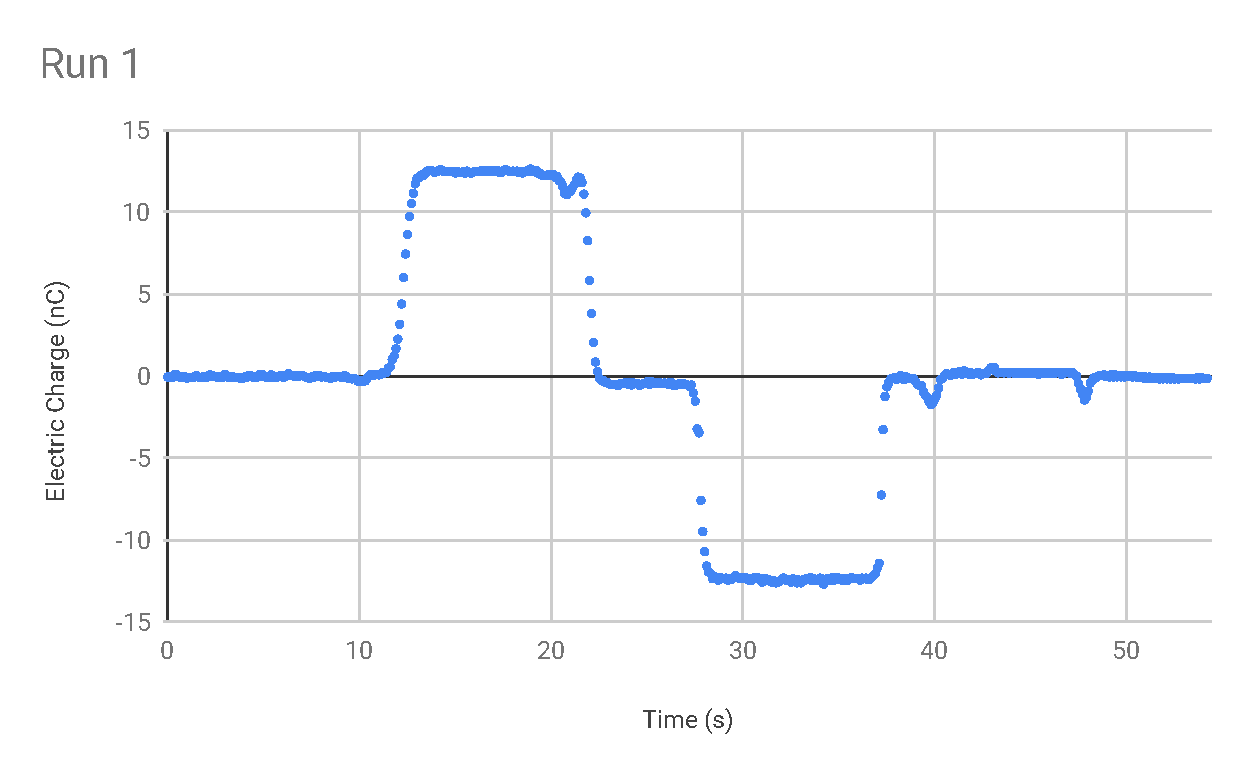
\includegraphics[scale=0.74]{image/01-electro/Run1.pdf}
	\caption{Run 1}
	\label{figure.01.run.1}
\end{figure}
%
\begin{figure}[ht]
	\centering
	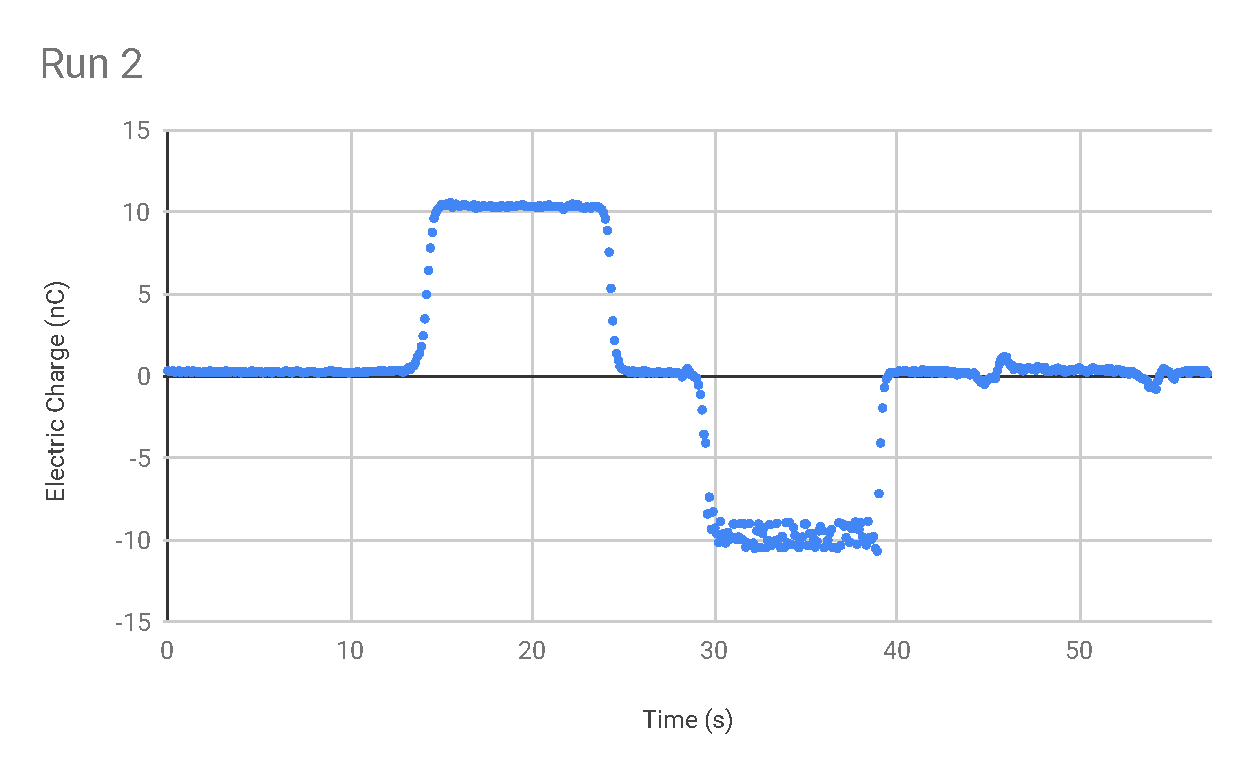
\includegraphics[scale=0.74]{image/01-electro/Run2.pdf}
	\caption{Run 2}
	\label{figure.01.run.2}
\end{figure}
%
\begin{figure}[ht]
	\centering
	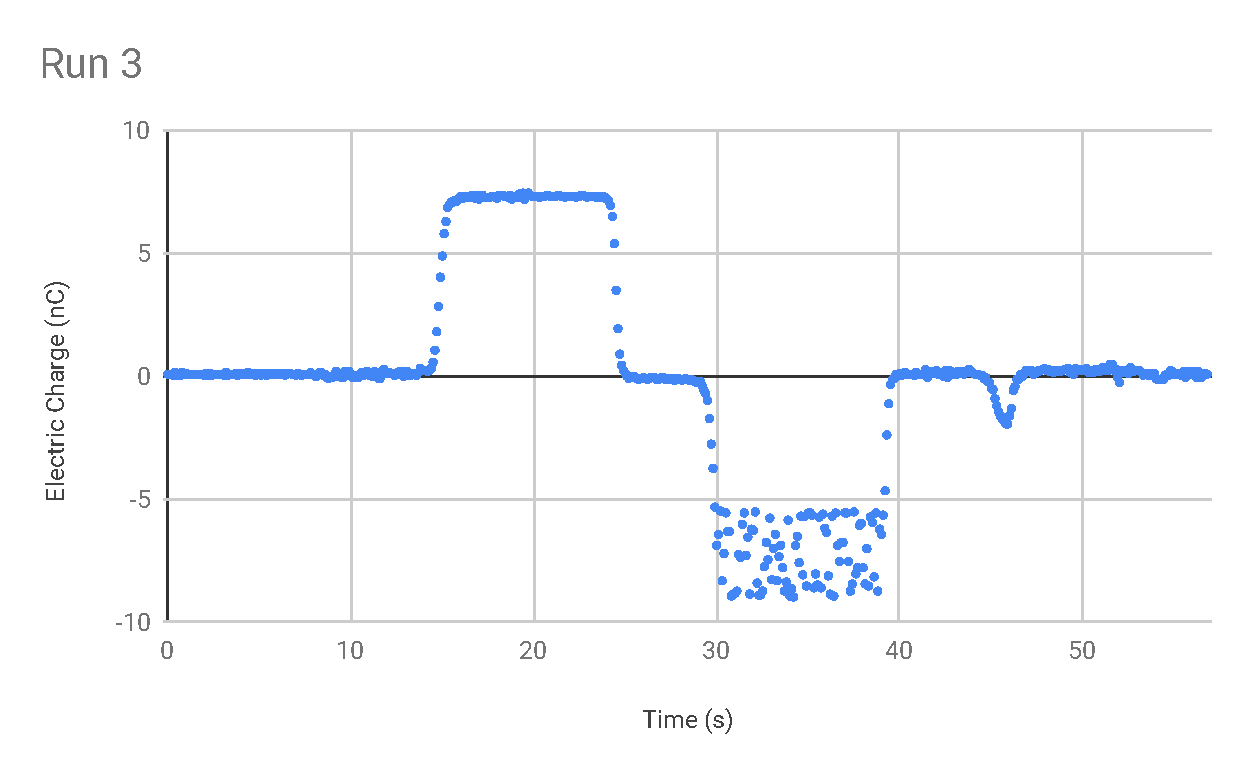
\includegraphics[scale=0.74]{image/01-electro/Run3.pdf}
	\caption{Run 3}
	\label{figure.01.run.3}
\end{figure}
%
\begin{figure}[ht]
	\centering
	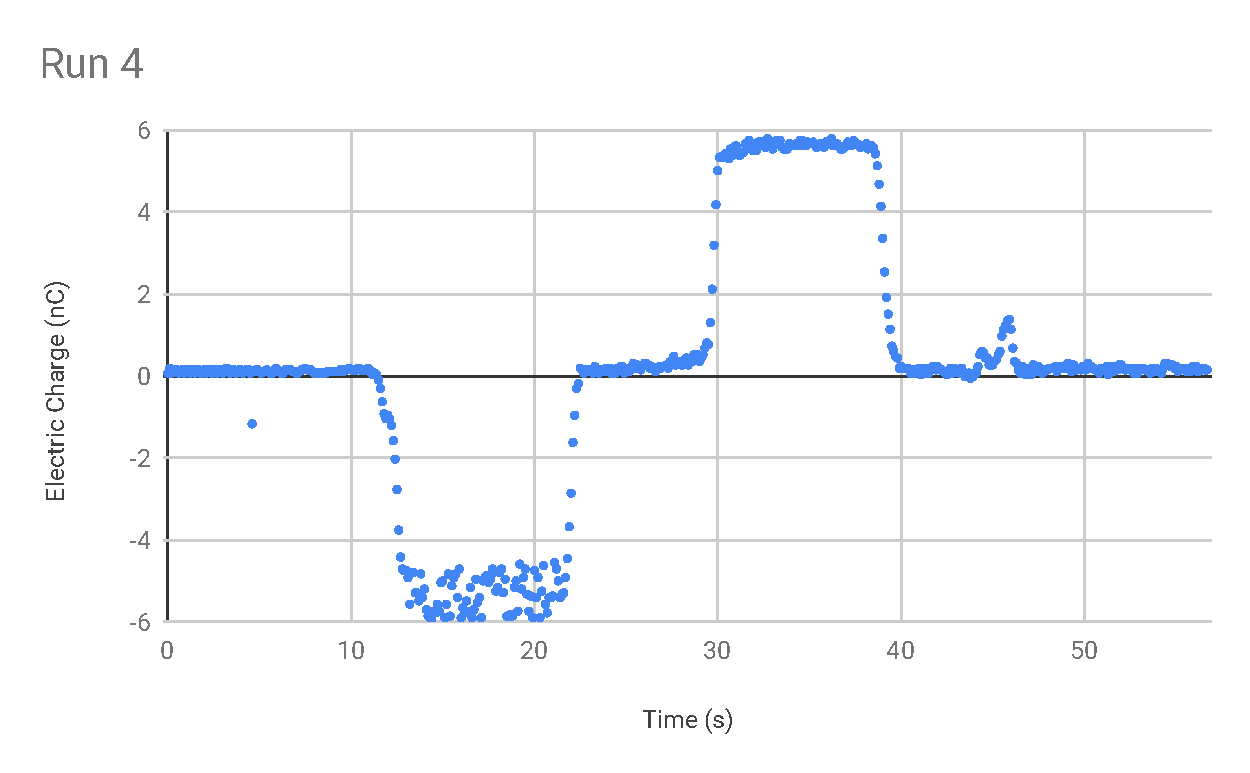
\includegraphics[scale=0.74]{image/01-electro/Run4.pdf}
	\caption{Run 4}
	\label{figure.01.run.4}
\end{figure}
%
\begin{figure}[ht]
	\centering
	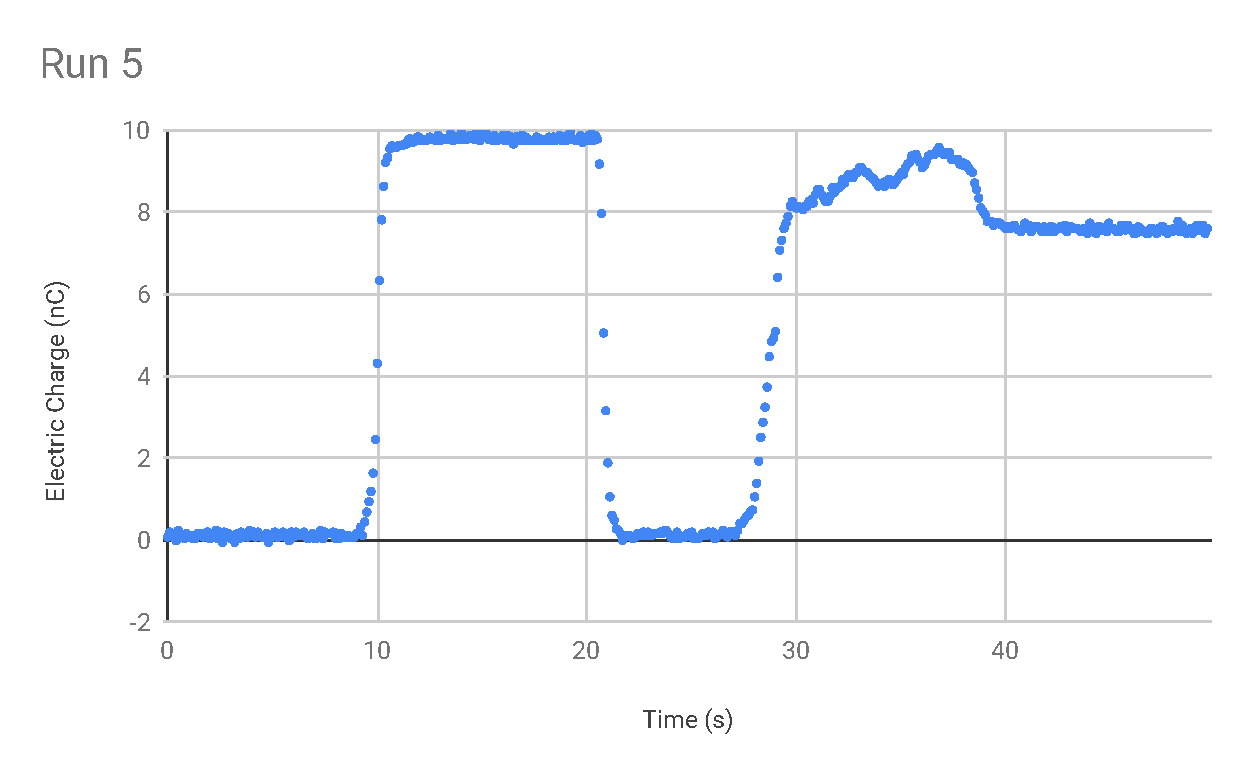
\includegraphics[scale=0.74]{image/01-electro/Run5.pdf}
	\caption{Run 5}
	\label{figure.01.run.5}
\end{figure}
%
\begin{figure}[ht]
	\centering
	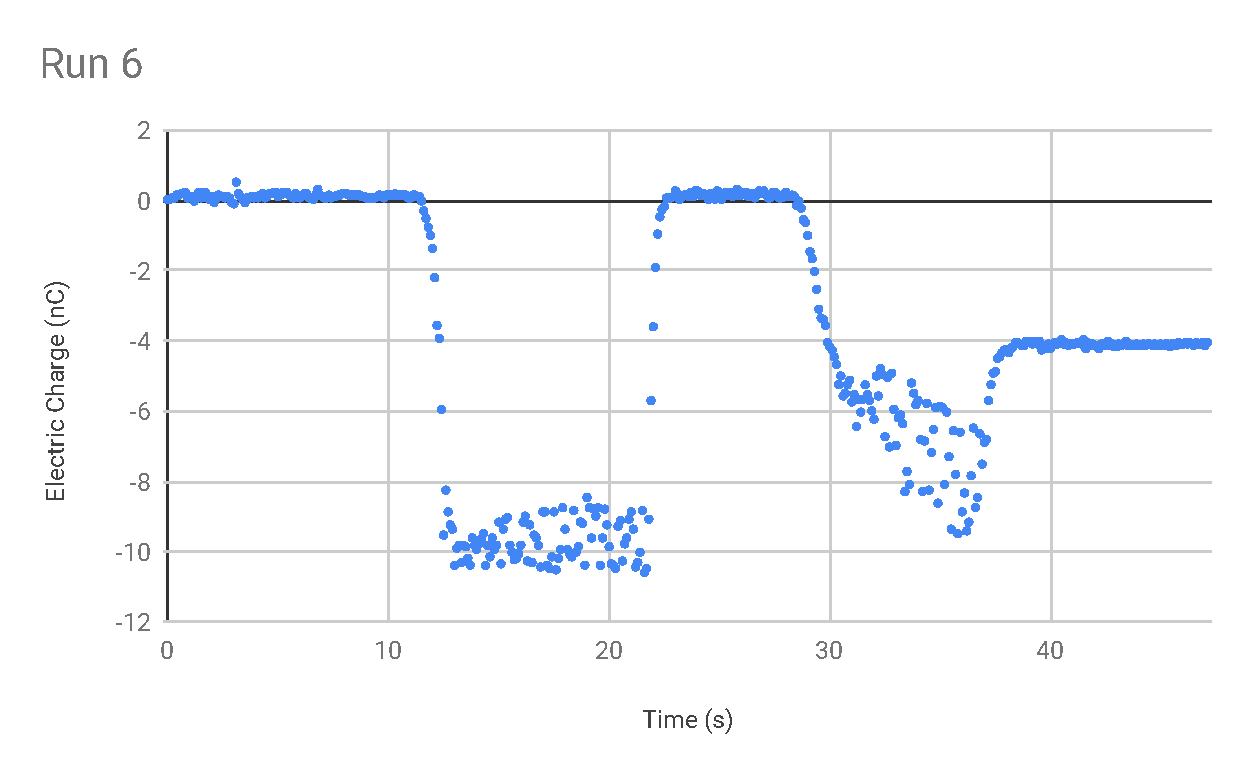
\includegraphics[scale=0.74]{image/01-electro/Run6.pdf}
	\caption{Run 6}
	\label{figure.01.run.6}
\end{figure}
%
\begin{figure}[ht]
	\centering
	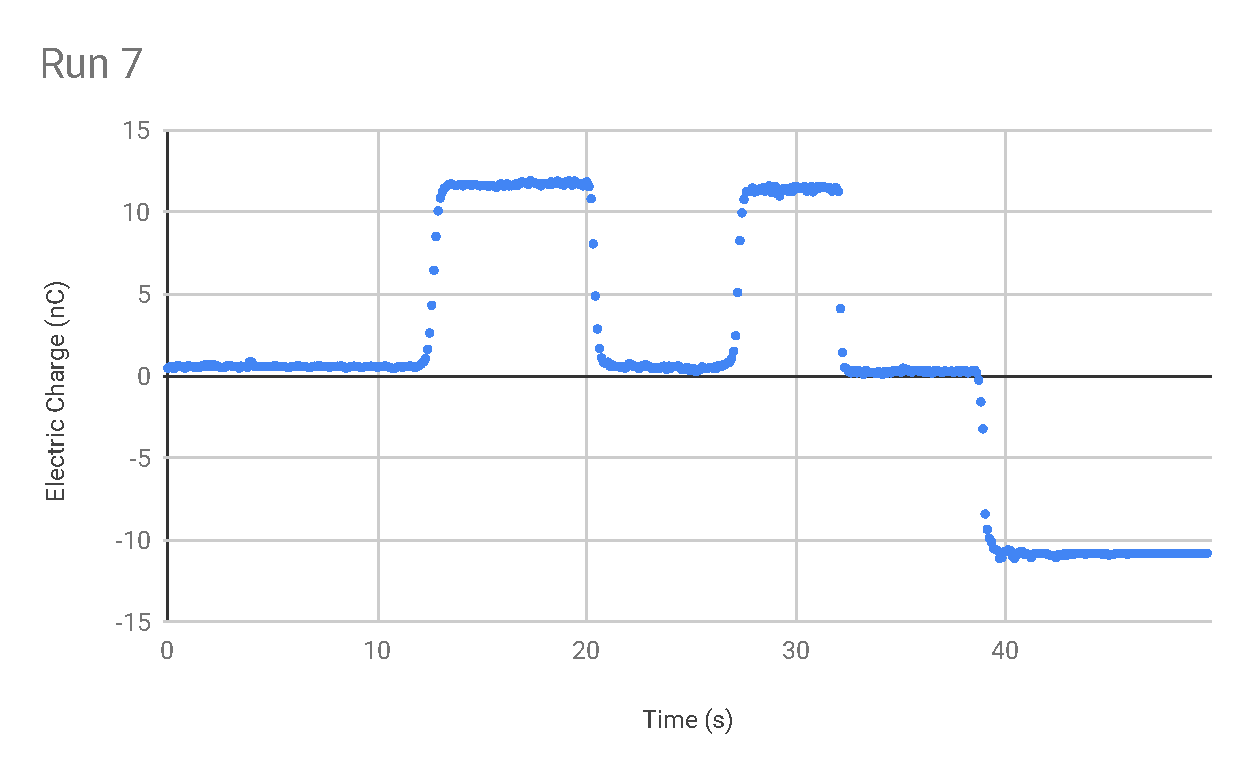
\includegraphics[scale=0.74]{image/01-electro/Run7.pdf}
	\caption{Run 7}
	\label{figure.01.run.7}
\end{figure}
%
\begin{figure}[ht]
	\centering
	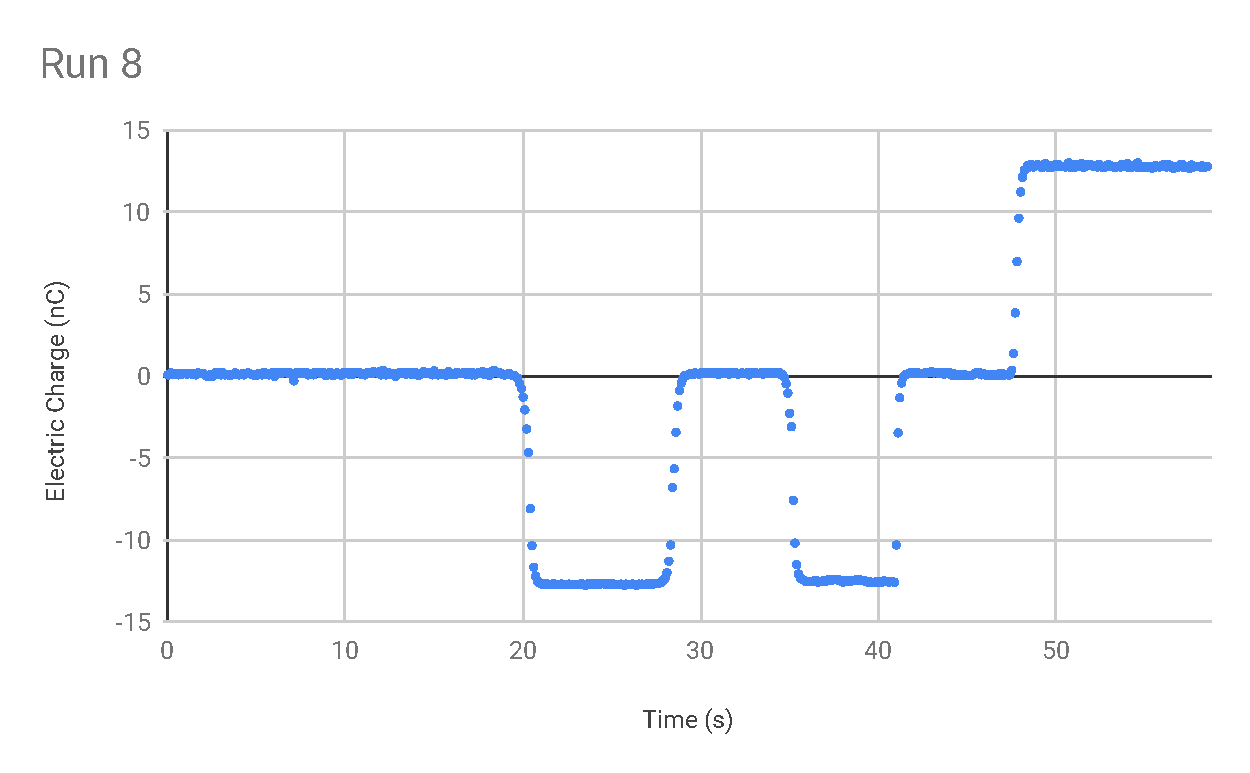
\includegraphics[scale=0.74]{image/01-electro/Run8.pdf}
	\caption{Run 8}
	\label{figure.01.run.8}
\end{figure}
%
% % Copyright 2018-2020 Melvin Eloy Irizarry-Gelpí
\setcounter{chapter}{1}
\chapter{Factors Affecting Electrical Resistance}
%
In this experiment you will learn about electrical resistance and resistivity.
%
\section{Preliminary}
%
At the microscopic level, the sources of electric charge are inside atoms. You have the \textbf{electron cloud}, with \textbf{negative} charges, and the \textbf{nucleus}, with \textbf{positive} charges (and also neutral charges that help keep the nucleus together). The atoms inside a typical piece of solid matter are arranged in a way such that the nuclei are held in place and do not move much but the electrons can jump to other atoms. In this sense, electric charge can flow through a material.

How easy it is for electrons to jump between atoms depends on how the atoms in a solid are arranged, and on how tightly the atom is holding on to the electron cloud. Depending on your goal, you might want to use a material that allows charges to move more easily (e.g. if you want to add wiring to your home). Electrical \textbf{resistance} and \textbf{resistivity} are two quantities that allow you to quantify and compare the ease of electric charge flow through a material. Before introducing the units used to measure these two quantities, it is useful to briefly mention other important electrical quantities.

Recall that the SI unit for \textbf{electric charge} is the coulomb (C). The coulomb is a fundamental unit that cannot be defined in terms of other SI units.
%
\subsection{Electric Potential and Voltage}
%
The Coulomb force can turn electric potential energy into work. The SI unit for energy is the joule (J). The amount of electric potential energy per unit of electric charge is known as the \textbf{electric potential}. Since energy is in J and electric charge is in C, the unit for electric potential is J/C. This combination of units is known as a \textbf{volt} (symbol is V):
\begin{equation}
	1 \text{ volt} = 1 \text{ V} = 1 \text{ J/C} = 1 \text{ joule per coulomb}
\end{equation}
The volt is the \textbf{SI unit} for electric potential. Electric potential, like energy, does not have a direction associated to it. Every point in space has a value of electric potential. If point 1 in space has an electric potential of $V_{1}$ and point 2 in space has an electric potential of $V_{2}$, then we say that there is a voltage $\Delta V$ given by
\begin{equation}
	\Delta V = V_{2} - V_{1}
\end{equation}
That is, a \textbf{voltage} is a difference of electric potential between two points in space. Technically speaking, absolute electric potential is not directly measurable, but voltage is.

The mathematical symbol for electric potential is $V$.
%
\subsection{Electric Current}
%
Another important quantity is \textbf{electric current}. Electric current quantifies the rate of flow (through a point in space) of electric charge with respect to time. Since electric charge is in coulombs and time is in seconds, the SI unit for electric current is C/s. This combination of units is known as an \textbf{ampere} (symbol is A):
\begin{equation}
	1 \text{ A} = 1 \text{ C/s}
\end{equation}
Although flow of charge in space suggests a direction is involved, the electric current is \textbf{not a vector} quantity.

The mathematical symbol for electric current is $I$.
%
\subsection{Electrical Resistance}
%
After introducing electric potential and electric current, and the units used to measure these quantities, you are ready to formally discuss \textbf{electric resistance}. The point of electric resistance is to quantify how easy it is for a current to flow through a particular material. The \textbf{SI unit} for electrical resistance is the \textbf{ohm} (symbol is $\Omega$, the uppercase Greek letter omega). Electric resistance is not a fundamental quantity. The ohm unit can be stated in terms of volts and amps:
\begin{equation}
	1 \text{ ohm} = 1 \text{ V/A}
\end{equation}
This result suggests that electrical resistance can be found by taking an electric potential value, and dividing it by an electric current value. This is not always the case.

When a piece of material has a large value of electrical resistance, it means that it is harder to get an electric current to flow through that piece of material. Small values of electrical resistance mean that it is easier for electric current to flow.

The mathematical symbol for electrical resistance is $R$.
%
\subsection{Ohm's Law}
%
Many materials, but not all of them, satisfy \textbf{Ohm's law}: the amount of electric potential difference $V$ across a piece of material is directly proportional to the amount of electric current $I$ flowing through the material:
\begin{equation}
	V = IR
\end{equation}
As you can see, the slope in this relation is a quantity with units of electrical resistance, and indeed corresponds to the electric resistance of the material. When such a relation holds, the material is said to be \textbf{ohmic}. For ohmic materials, the electrical resistance $R$ can be calculated from the amount of electric potential difference $V$ and electric current $I$ via
\begin{equation}
	R = \frac{V}{I}
	\label{eq.02.ohms.law}
\end{equation}
Not all materials are ohmic. That means that not all ratios of the form $V/I$ can be interpreted as electrical resistance.
%
\subsection{Geometry of a Cylinder}
%
Each distinct material has its own value of electrical resistance. As you will find during this experiment, electrical resistance not only depends on the kind of material being use, but also on the \textbf{geometrical} aspects of the particular piece of material under study.

To a good approximation, almost all electrical wires have a cylindrical shape. A \textbf{cylinder} is a shape with a \textbf{length} $l$ and a circular base with \textbf{area} $A$. The area of a circle is
\begin{equation}
	A = \frac{1}{4} \pi d^{2}
	\label{eq.02.area}
\end{equation}
Here $d$ is the \textbf{diameter} of the circular base. Recall that the diameter of a circle is twice its radius, and that the radius of a circle is the distance from the center of the circle to any point on the circle. It turns out that the electrical resistance of a cylindrical wire depends on the length $l$ and the area $A$ of the cylinder.
%
\subsection{Electrical Resistivity}
%
For convenience, it is useful to introduce a quantity called \textbf{electrical resistivity} that is similar to electrical resistance, but does not depend on the geometrical aspects of the particular piece of material. In this way, electrical resistivity is \textbf{more intrinsic} than electrical resistance. The \textbf{SI unit} for electrical resistivity is the ohm$\cdot$meter (i.e. ohm multiply by meter).

The mathematical symbol for electrical resistivity is $\rho$ (the lowercase Greek letter rho).
%
\section{Experiment}
%
The main goal of this experiment is to study and understand how the electrical resistance $R$ of a cylindrical wire depends on the length $l$ of the wire, and the area $A$ of the cross-section of the wire. In principle, you would measure $R$, $l$, and $A$, and then make a chart. In practice you cannot measure $R$ directly. Instead you measure electric potential and electric current directly, and then use Ohm's law (\ref{eq.02.ohms.law}) to calculate $R$.

You have eight different rods. Four of them are made of brass (but these four brass rods have different diameter), the other four are made of other materials (but these four rods have the same diameter).
%
\subsection{Part 1: Effect of Length}
%
In the first part you keep the material and the area fixed, and consider different lengths:
\begin{itemize}
	\item Run 1: Brass, $d = 3.18$ mm
\end{itemize}
You should consider about six different length values.
%
\subsection{Part 2: Effect of Material}
%
In the second part you change the material, but keep the area fixed, and consider different lengths for each material:
\begin{itemize}
	\item Run 2: Copper, $d = 3.18$ mm
	\item Run 3: Music Wire, $d = 3.18$ mm
	\item Run 4: Aluminum, $d = 3.18$ mm
	\item Run 5: Stainless Steel, $d = 3.18$ mm
\end{itemize}
For each material you should consider six different length values.
%
\subsection{Part 3: Effect of Area}
%
In the third part you keep the material fixed, and consider different areas:
\begin{itemize}
	\item Run 6: Brass, $d = 2.38$ mm
	\item Run 6: Brass, $d = 3.97$ mm
	\item Run 8: Brass, $d = 4.76$ mm
\end{itemize}
For each rod you should consider six different length values.
%
\section{Analysis}
%
Many \textbf{non-SI units} are used in this experiment, mostly for convenience reasons:
\begin{itemize}
	\item Length along the rod is in centimeters (cm).
	\item Diameter of the rod is in millimeters (mm).
	\item Electric potential along rod segment is in millivolts (mV).
\end{itemize}
Recall that
\begin{align}
	1 \text{ cm} = 0.01 \text{ m} && 1 \text{ mm} = 0.001 \text{ m} && 1 \text{ mV} = 0.001 \text{ V}
\end{align}
It is very important that SI units are used before any calculations, so that the resistance comes out in ohm units and the resistivity comes out in ohm$\cdot$meter units.
%
\subsection{Part 1 and Part 2: Length}
%
Here is what to do for runs 1, 2, 3, 4, and 5.
%
\subsubsection{Convert the units of potential to SI units}
%
The LabQuest device will measure the electric potential in units of millivolts (mV). In a separate column, convert these values to units of volts (V) by multiplying each millivolt value by a factor of $0.001$.
%
\subsubsection{Calculate the resistance in ohms}
%
With the current in amps, and the potential in volts, you can calculate the resistance in ohms by using (\ref{eq.02.ohms.law}).
%
\subsubsection{Convert the units of length to SI units}
%
You used the centimeter (cm) marks to measure the length along the rod where the electric potential measurement was taken. In a separate column, convert these values to units of meters (m) by multiplying each centimeter value by a factor of $0.01$.
%
\subsubsection{Make a chart of $R$ versus $l$}
%
It is time to visualize the data. Make a scatter chart with resistance in the vertical axis, and length in the horizontal axis. Label both axes and add a title to each chart that includes the run number, the material being used, and the value of the diameter.
%
\subsubsection{Calculate the slope of the best-fit line}
%
If the shape of the data is linear, include a \textbf{best-fit line}. In a separate cell, use \texttt{SLOPE} to calculate the value of the slope. If the linear fit is appropriate, this suggest that the amount of resistance $R$ is directly proportional to the amount of length $l$:
\begin{equation}
	R = a_{1} l + b_{1}
\end{equation}
Here, $a_{1}$ is the slope and $b_{1}$ is the intercept. The slope $a_{1}$ should have ohm/m units, and the intercept $b_{1}$ should have ohm units.

Note that the area $A$ was kept constant.
%
\subsection{Part 3: Area}
%
For runs 6, 7, and 8 you should do the same steps as those for the previous runs. Along with run 1, for each length value you should have four values for resistance and area. Here is what to do after you have the resistance versus length values.
%
\subsubsection{Convert the units of diameter to SI units}
%
The diameter of each rod is given in units of millimeters (mm). In a separate column, convert these values to units of meter (m) by multiplying each millimeter value by a factor of $0.001$.
%
\subsubsection{Calculate the area in m$^{2}$}
%
With the diameter in meter units, you can calculate the area using (\ref{eq.02.area}). For $\pi$ you can use \texttt{PI()} instead of writing the value by hand.
%
\subsubsection{Calculate the inverse area in 1/m$^{2}$}
%
It is going to be important to calculate the inverse area. In a separate column, calculate the reciprocal inverse of each area value.
%
\subsubsection{Make a chart of $R$ versus $1/A$}
%
Choose a length value, then gather the corresponding resistance value from runs 1, 6, 7, and 8. You should have resistance for four different areas (or inverse areas).

If you make a chart with $R$ in the vertical axis, and $A$ in the horizontal axis, you will find that although there is a pattern, it is not a linear pattern (see Figure \ref{figure.02.10cm.non.linear}). Instead, the chart with $R$ in the vertical axis, and $1/A$ in the horizontal axis does show a linear pattern.
%
\subsubsection{Calculate the slope of the best-fit line}
%
A linear shape suggests that $R$ is directly proportional to $1/A$:
\begin{equation}
	R = \frac{a_{2}}{A} + b_{2}
\end{equation}
Here $a_{2}$ is the slope and $b_{2}$ is the intercept. The slope $a_{2}$ should have ohm$\cdot$m$^{2}$ units, and the intercept $b_{2}$ should have ohm units.

Note that the length $l$ was kept constant.
%
\subsection{Part 4: Resistivity}
%
Keeping the area fixed and letting the length vary yielded the following linear relation:
\begin{equation}
	R = a_{1} l + b_{1}
\end{equation}
Keeping the length fixed and letting the area vary yielded the following linear relation:
\begin{equation}
	R = \frac{a_{2}}{A} + b_{2}
\end{equation}
Ignoring the intercepts, this suggests a relation of the form:
\begin{equation}
	R = a_{3} \frac{l}{A}
\end{equation}
Here $a_{3}$ has ohm$\cdot$m units, the same units as resistivity. This suggests that $a_{3}$ corresponds to the resistivity.

You can now go back to your results and compute the resistivity from the $a_{1}$ value by multiplying it by the corresponding area:
\begin{equation}
	\rho = a_{1} A
\end{equation}
Similarly, you can compute the resistivity from the $a_{2}$ value by dividing it by the corresponding length:
\begin{equation}
	\rho = \frac{a_{2}}{l}
\end{equation}
In principle, these two methods of obtaining the resistivity should yield very similar values.
%
\subsection{Comparisons with Established Results}
%
Your experimental results for the electrical resistivity can be compared to established values. See Table \ref{table.02.established}. The values for brass, copper, and aluminum were taken from this \href{http://www.radio-electronics.com/info/formulae/resistance/resistivity-table.php}{website}. The value for stainless steel and music wire was taken from \href{https://en.wikipedia.org/wiki/Electrical_resistivity_and_conductivity}{Wikipedia}. Since some kinds of music wire is made with carbon steel, you can compare the resistivity of music wire to the resistivity of carbon steel.
%
\section{My Data}
%
Keeping the area fixed, you can find the electrical resistivity for each of the eight runs. Table \ref{table.02.experimental.area} contains my results. Each resistivity is found by multiplying the value of the slope from the best-fit line by the corresponding area. For example, Figure \ref{figure.02.run.1} has the data for run 1. The slope is $4.97 \times 10^{-3}$ ohm/m. The diameter is 3.18 mm, giving an area of $7.96 \times 10^{-6}$ m$^{2}$. The resistivity is
\begin{equation}
	\rho = \left(4.97 \times 10^{-3} \text{ ohm/m}\right) \left(7.96 \times 10^{-6} \text{ m}^{2}\right) = 7.35 \times 10^{-8} \text{ ohm}\cdot\text{m}
\end{equation}
From the $R$ versus $1/A$ charts, you have to divide the slope by the length to obtain the resistivity. For example, Figure \ref{figure.02.20cm} has the data for brass, keeping the length fixed at 20 cm. The slope is $1.58 \times 10^{-8}$ ohm$\cdot$m$^{2}$. The length is 0.2 m. The resistivity is
\begin{equation}
	\rho = \frac{1.58 \times 10^{-8} \text{ ohm}\cdot\text{m}^{2}}{0.2 \text{ m}} = 7.50 \times 10^{-8} \text{ ohm}\cdot\text{m}
\end{equation}
You expect the value of the resistivity to be independent on how it is calculated. Indeed, both of the values above are very close and consistent.
%
\section{Your Data}
%
You should have eight runs, similar to my eight runs of data.
%
\newpage
\section{Your Lab Report}
%
In your laboratory report you should include the following:
\begin{enumerate}
	\item A table like Table \ref{table.02.experimental.area} with the resistivity values for each run with fixed area.
	\item A table like Table \ref{table.02.experimental.length} with the resistivity values for \textbf{three} distinct lengths.
	\item Discuss whether your experimental values for the resistivity agree with established values (see Table \ref{table.02.established}).
	\item Two scatter charts with electrical resistance in the vertical axis, and length in the horizontal axis (similar to Figure \ref{figure.02.run.1}). Include the best-fit line and display the equation.
	\item One scatter chart with electrical resistance in the vertical axis, and inverse area in the horizontal axis (similar to Figure \ref{figure.02.15cm}). Include the best-fit line and display the equation.
	\item Which material resulted in the largest value of electrical resistivity? Include your answer in the report.
	\item Which material resulted in the smallest value of electrical resistivity? Include your answer in the report.
\end{enumerate}
%
\newpage
\section{Tables}
%
\begin{table}[ht]
	\centering
	\begin{tabular}{|l|r|}
		\hline
		Material & Resistivity (ohm$\cdot$m) \\
		\hline
		Brass & $6 \times 10^{-8}$ to $9 \times 10^{-8}$ \\
		Copper & $1.7 \times 10^{-8}$ \\
		Carbon Steel & $1.43 \times 10^{-7}$ \\
		Aluminum & $2.8 \times 10^{-8}$ \\
		Stainless Steel & $6.90 \times 10^{-7}$ \\
		\hline
	\end{tabular}
	\caption{Established values for electrical resistivity of some materials}
	\label{table.02.established}
\end{table}
%
\begin{table}[ht]
	\centering
	\begin{tabular}{|l|r|r|r|}
		\hline
		Run & Material & Diameter (mm) & Resistivity (ohm$\cdot$m) \\
		\hline
		1 & Brass & 3.18 & $7.35 \times 10^{-8}$ \\
		2 & Copper & 3.18 & $1.59 \times 10^{-8}$ \\
		3 & Carbon Steel & 3.18 & $1.89 \times 10^{-7}$ \\
		4 & Aluminum & 3.18 & $3.53 \times 10^{-8}$ \\
		5 & Stainless Steel & 3.18 & $7.06 \times 10^{-7}$ \\
		6 & Brass & 2.38 & $7.52 \times 10^{-8}$ \\
		7 & Brass & 3.97 & $7.44 \times 10^{-8}$ \\
		8 & Brass & 4.76 & $7.07 \times 10^{-8}$ \\
		\hline
	\end{tabular}
	\caption{Experimental values for electrical resistivity of some materials with fixed area}
	\label{table.02.experimental.area}
\end{table}
%
\begin{table}[ht]
	\centering
	\begin{tabular}{|l|r|}
		\hline
		Length (cm) & Resistivity (ohm$\cdot$m) \\
		\hline
		10 & $7.46 \times 10^{-8}$ \\
		15 & $7.56 \times 10^{-8}$ \\
		20 & $7.50 \times 10^{-8}$ \\
		25 & $7.63 \times 10^{-8}$ \\
		\hline
	\end{tabular}
	\caption{Experimental values for electrical resistivity of brass with fixed length}
	\label{table.02.experimental.length}
\end{table}
%
\FloatBarrier
\newpage
\section{Figures}
%
\begin{figure}[ht]
	\centering
	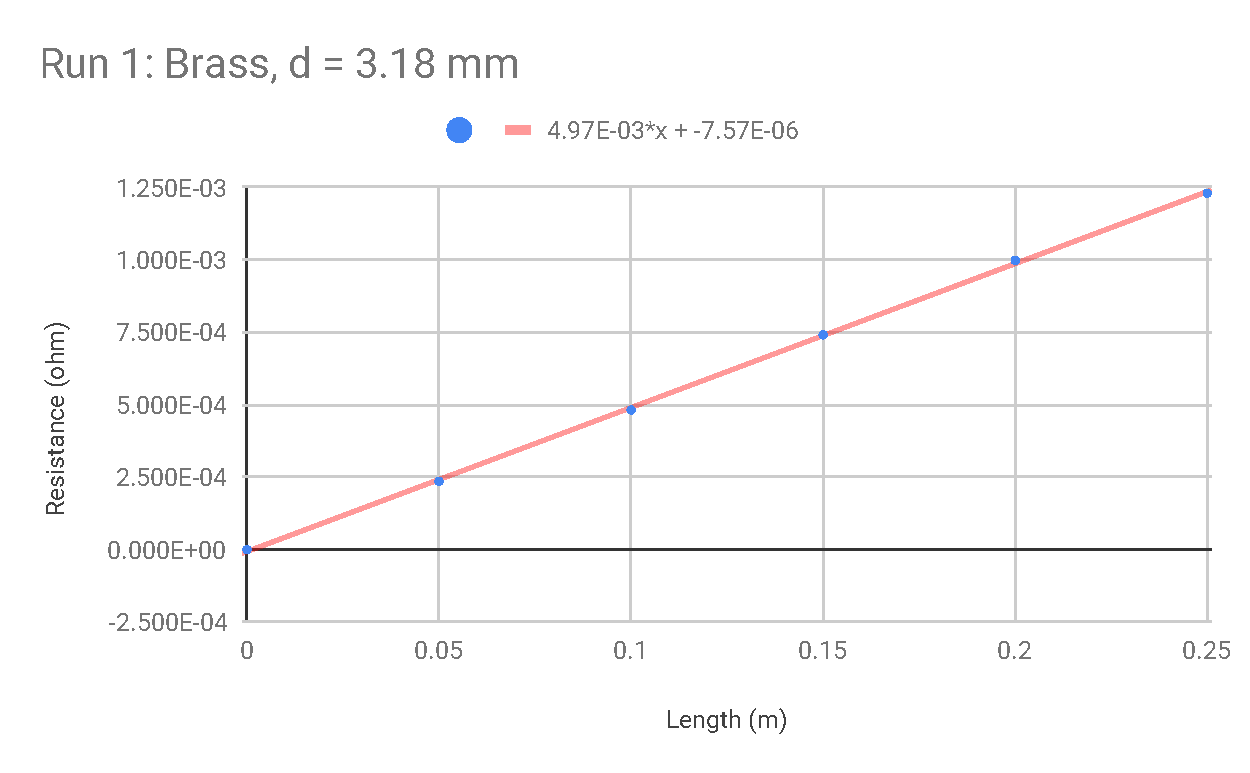
\includegraphics[scale=0.74]{image/02-resistance/run1.pdf}
	\caption{Run 1}
	\label{figure.02.run.1}
\end{figure}
%
\begin{figure}[ht]
	\centering
	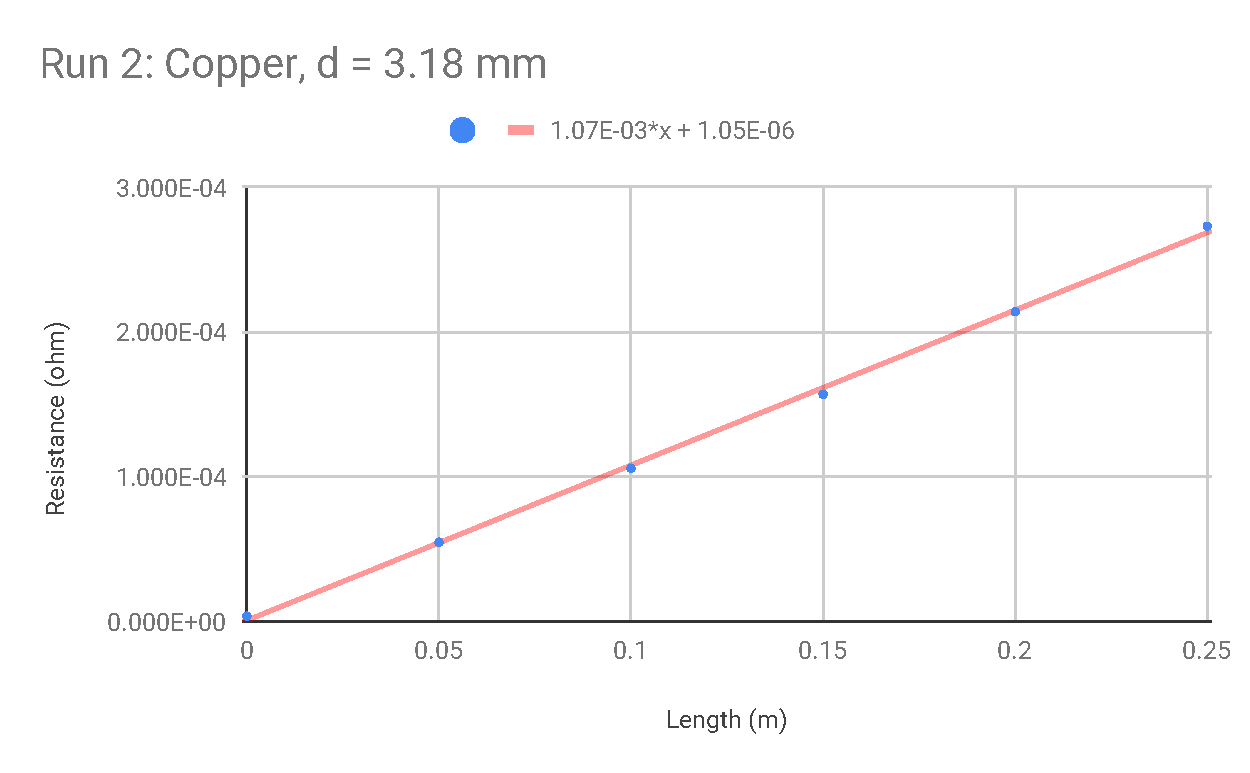
\includegraphics[scale=0.74]{image/02-resistance/run2.pdf}
	\caption{Run 2}
	\label{figure.02.run.2}
\end{figure}
%
\begin{figure}[ht]
	\centering
	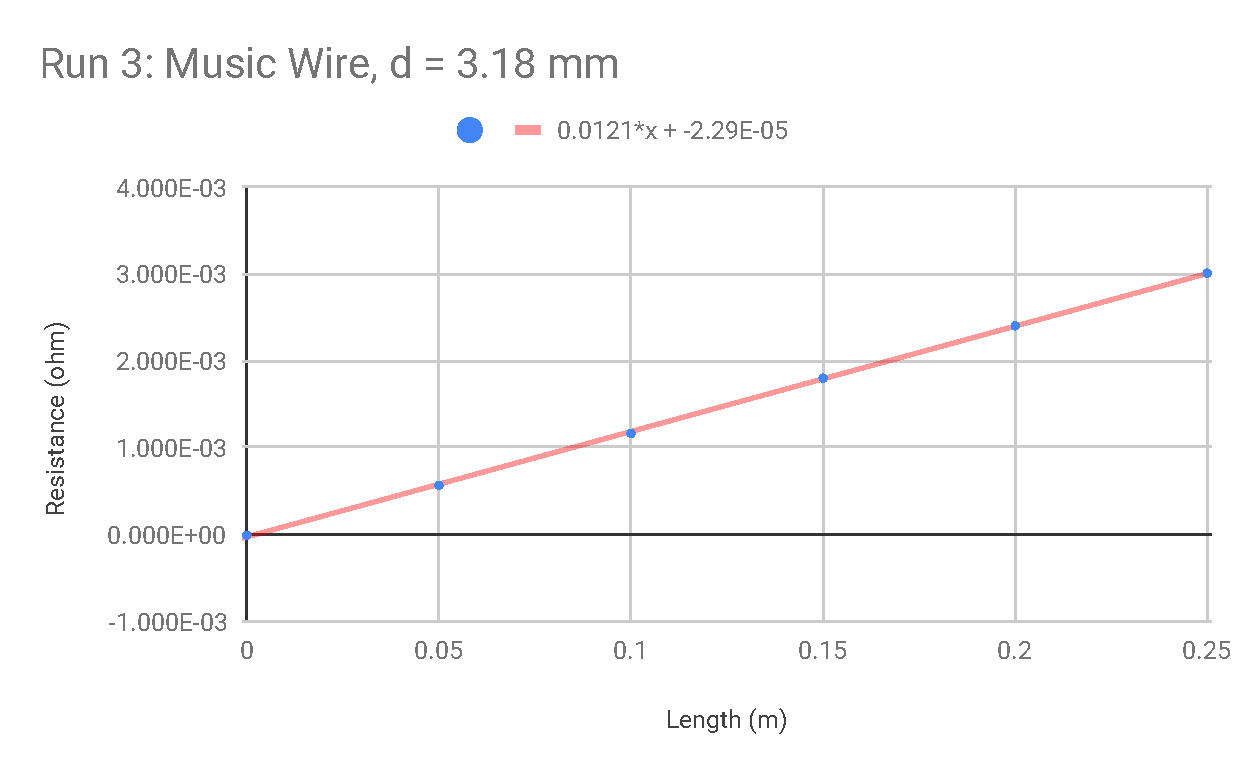
\includegraphics[scale=0.74]{image/02-resistance/run3.pdf}
	\caption{Run 3}
	\label{figure.02.run.3}
\end{figure}
%
\begin{figure}[ht]
	\centering
	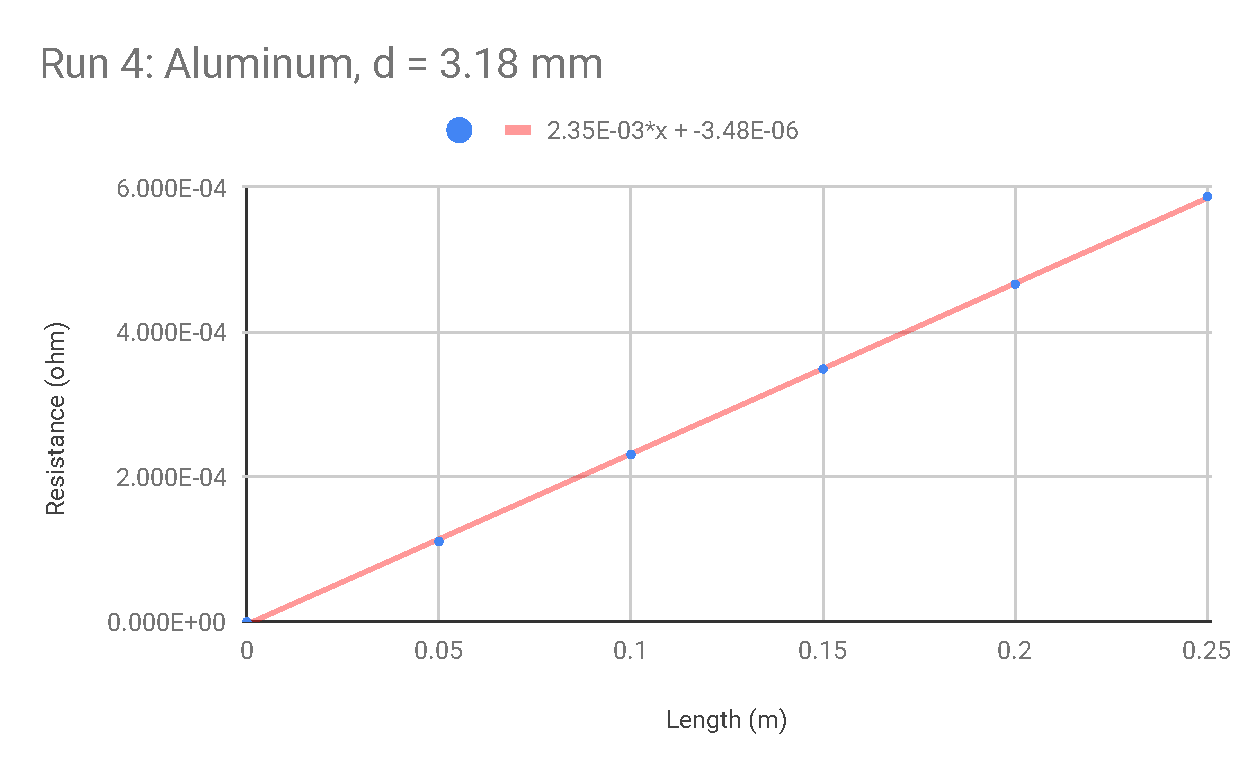
\includegraphics[scale=0.74]{image/02-resistance/run4.pdf}
	\caption{Run 4}
	\label{figure.02.run.4}
\end{figure}
%
\begin{figure}[ht]
	\centering
	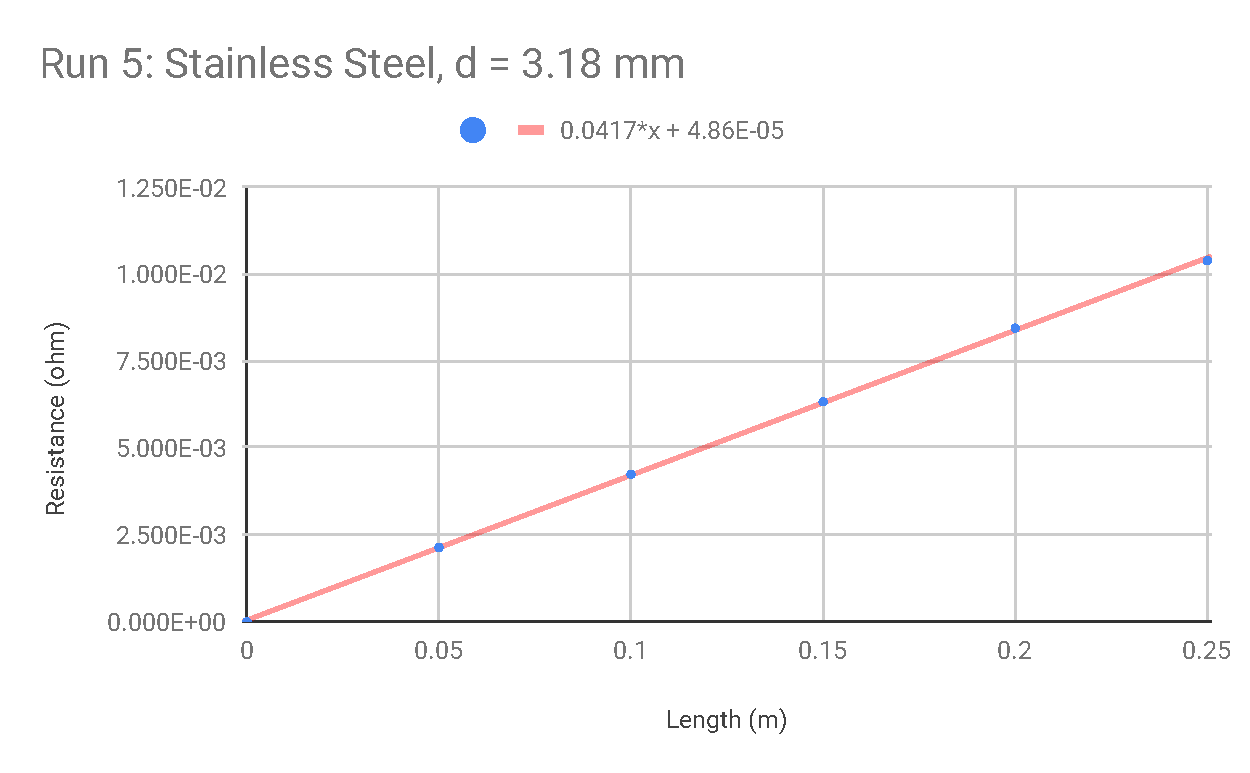
\includegraphics[scale=0.74]{image/02-resistance/run5.pdf}
	\caption{Run 5}
	\label{figure.02.run.5}
\end{figure}
%
\begin{figure}[ht]
	\centering
	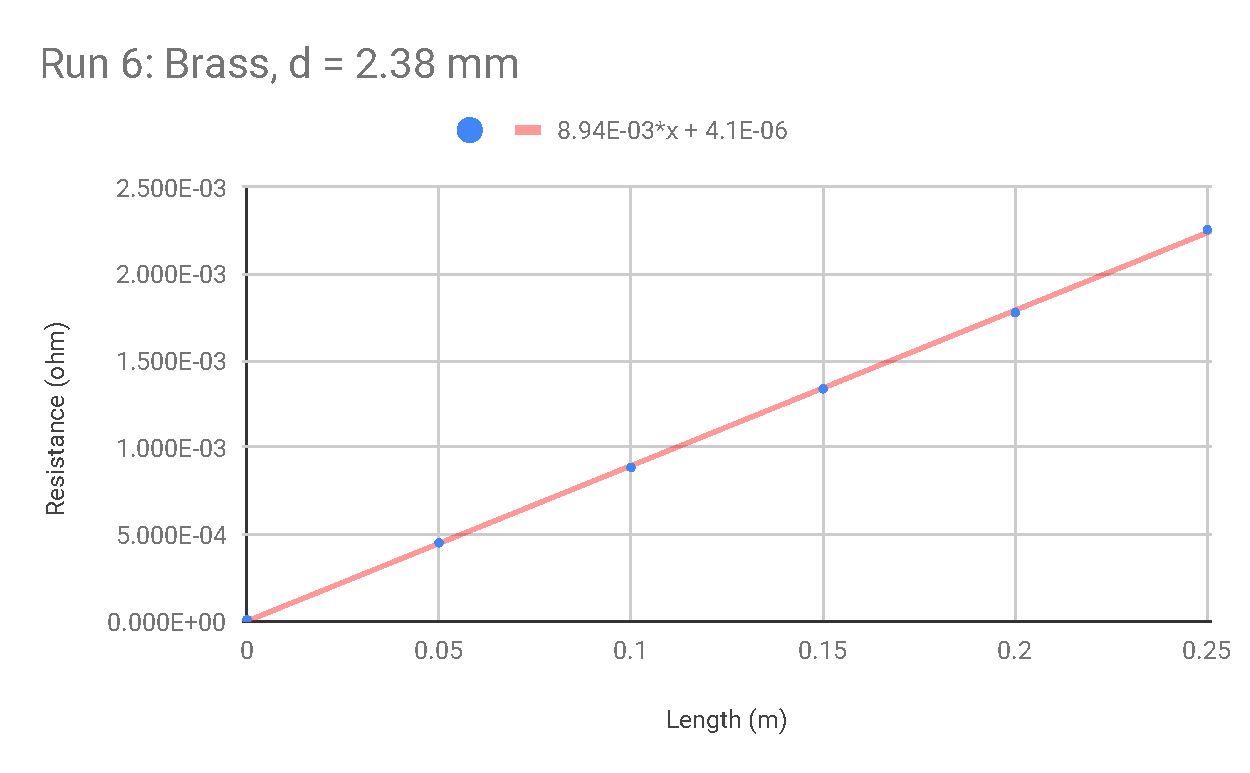
\includegraphics[scale=0.74]{image/02-resistance/run6.pdf}
	\caption{Run 6}
	\label{figure.02.run.6}
\end{figure}
%
\begin{figure}[ht]
	\centering
	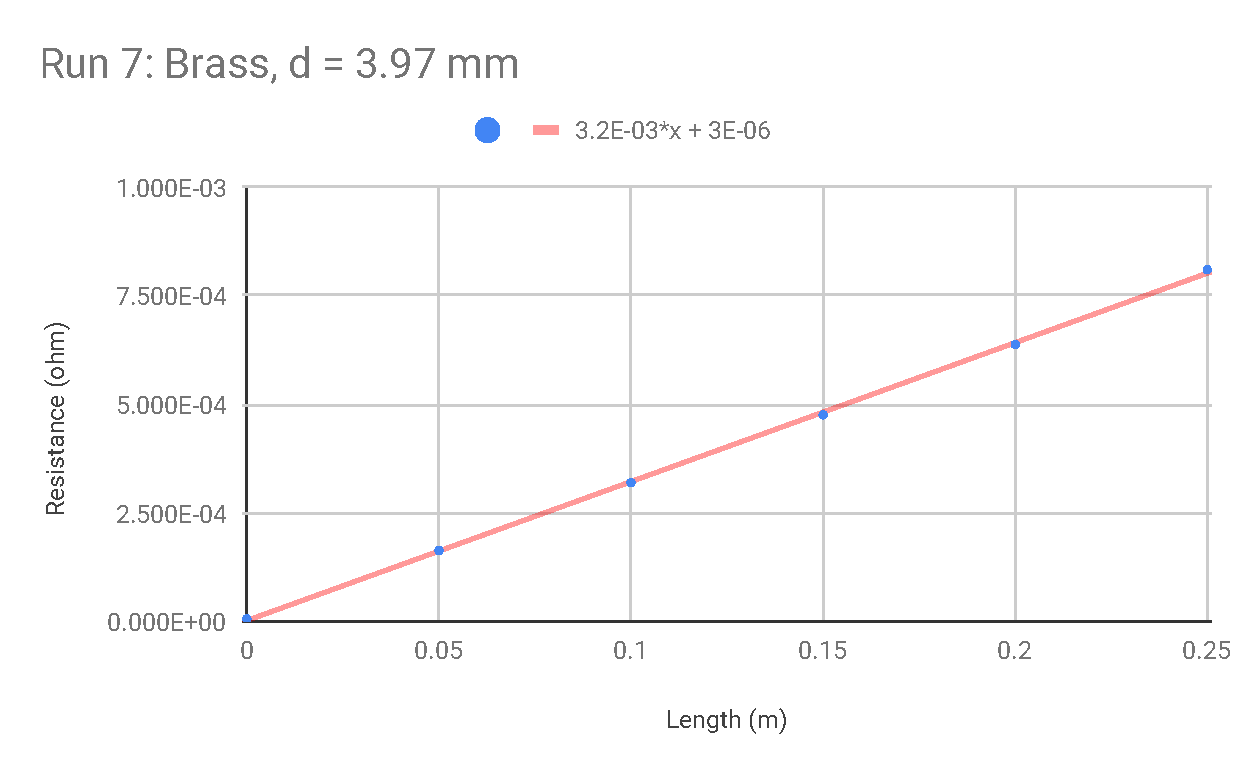
\includegraphics[scale=0.74]{image/02-resistance/run7.pdf}
	\caption{Run 7}
	\label{figure.02.run.7}
\end{figure}
%
\begin{figure}[ht]
	\centering
	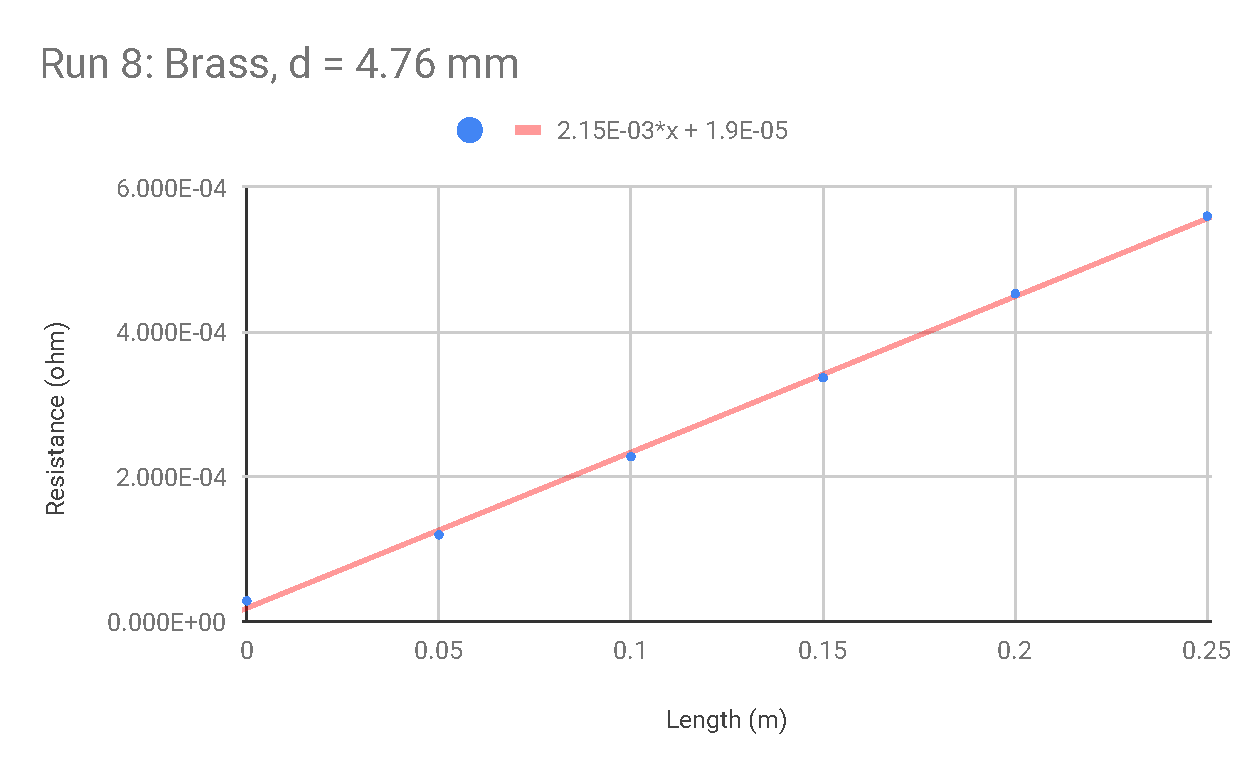
\includegraphics[scale=0.74]{image/02-resistance/run8.pdf}
	\caption{Run 8}
	\label{figure.02.run.8}
\end{figure}
%
\begin{figure}[ht]
	\centering
	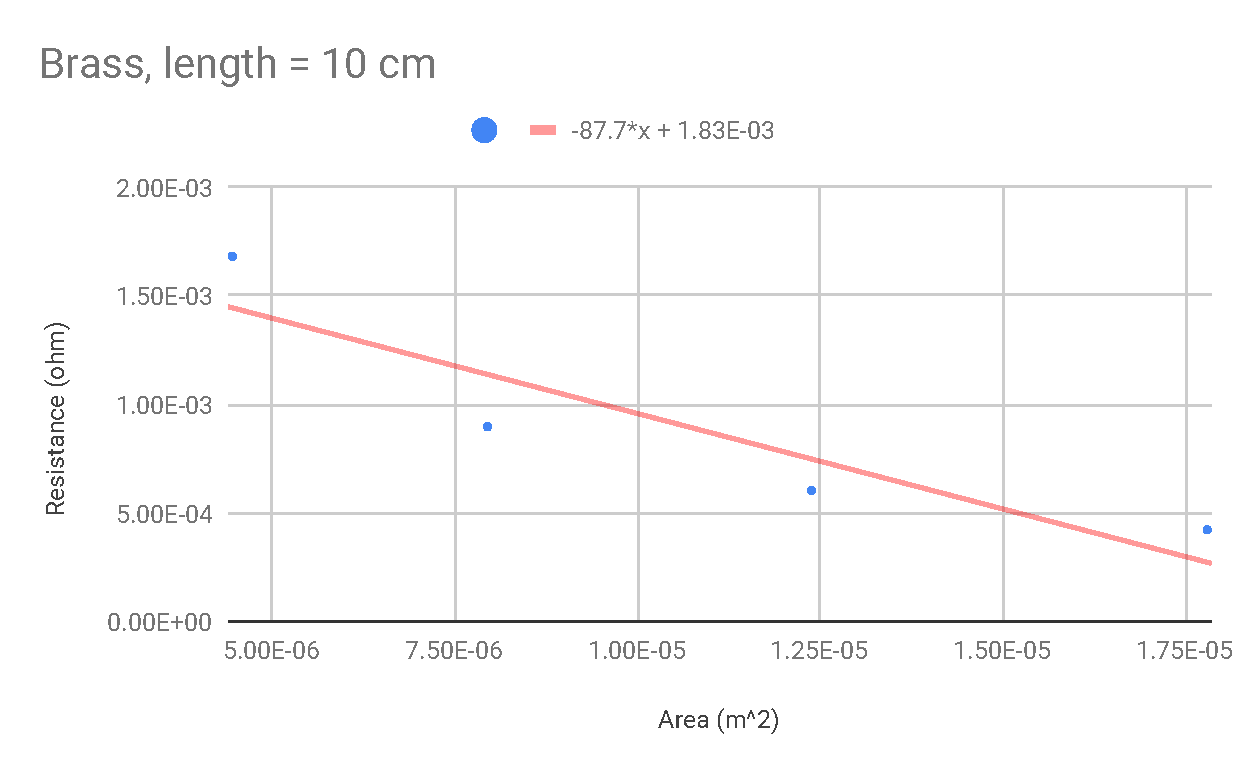
\includegraphics[scale=0.74]{image/02-resistance/10cm-non-linear.pdf}
	\caption{Brass, $l = 10$ cm, non-linear behavior}
	\label{figure.02.10cm.non.linear}
\end{figure}
%
\begin{figure}[ht]
	\centering
	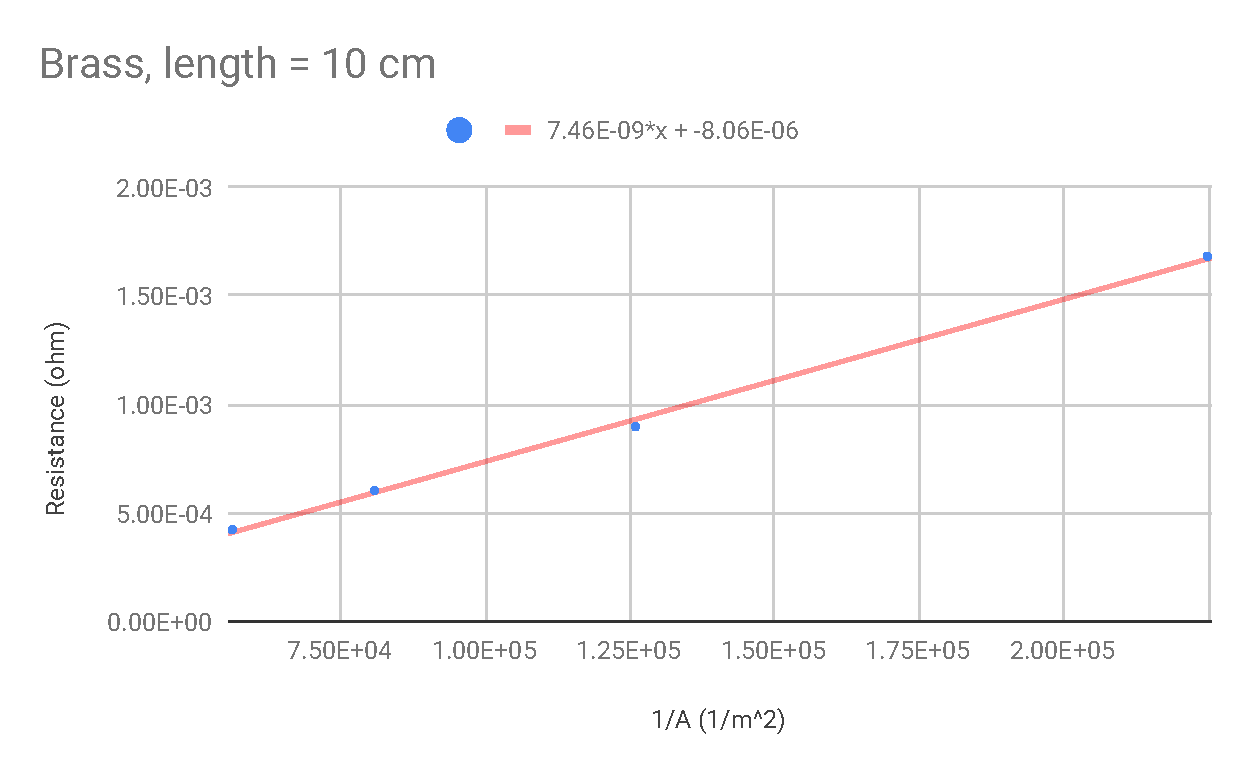
\includegraphics[scale=0.74]{image/02-resistance/10cm.pdf}
	\caption{Brass, $l = 10$ cm}
	\label{figure.02.10cm}
\end{figure}
%
\begin{figure}[ht]
	\centering
	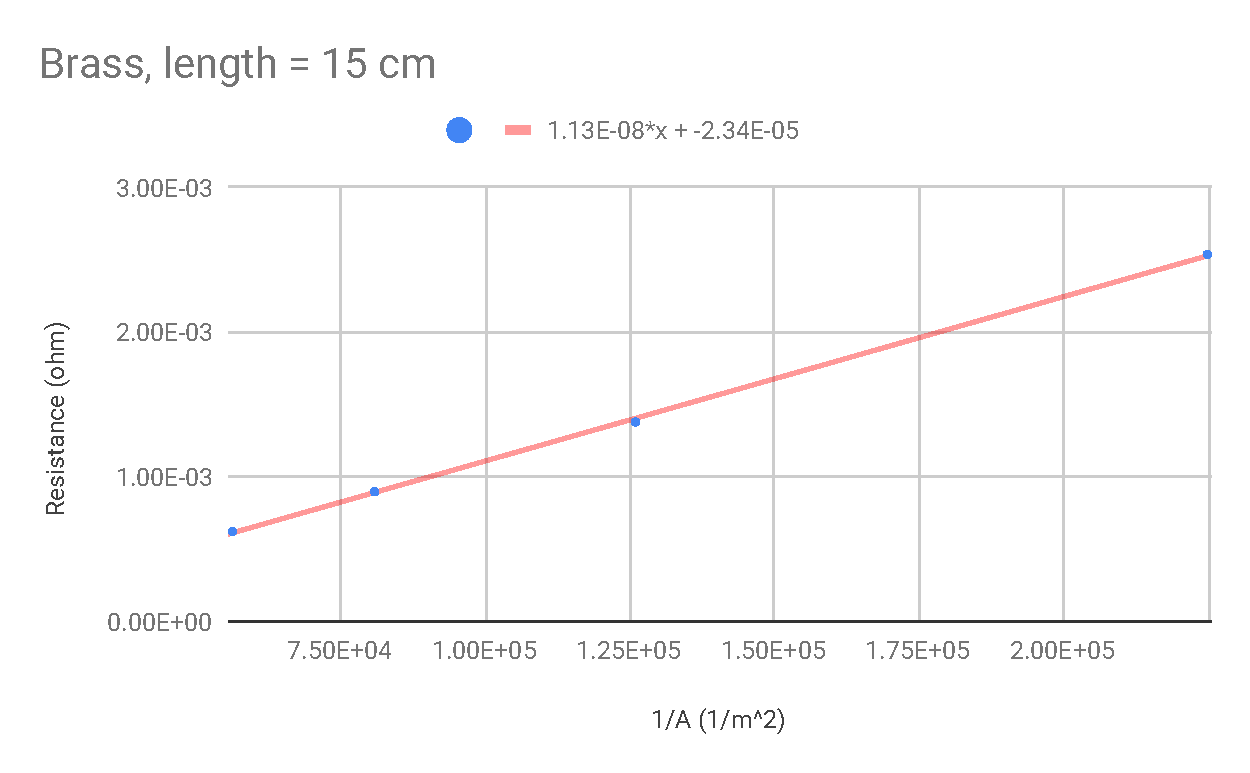
\includegraphics[scale=0.74]{image/02-resistance/15cm.pdf}
	\caption{Brass, $l = 15$ cm}
	\label{figure.02.15cm}
\end{figure}
%
\begin{figure}[ht]
	\centering
	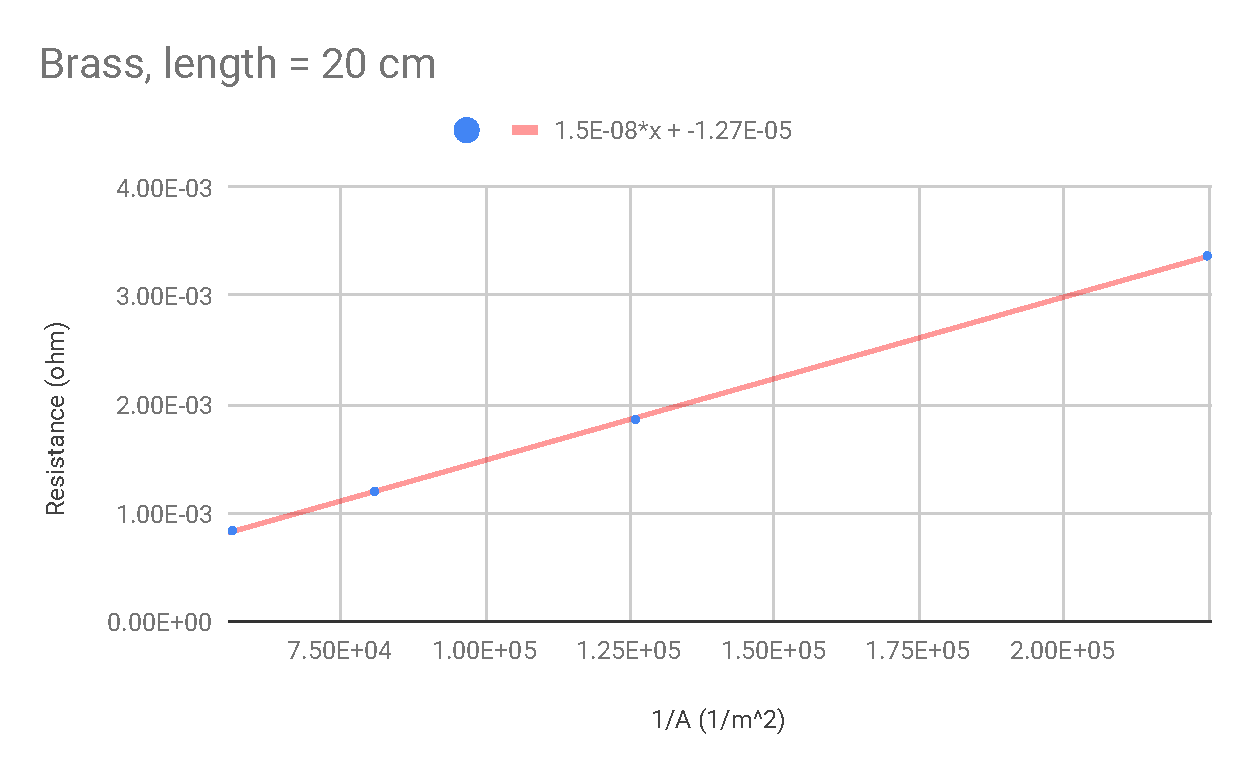
\includegraphics[scale=0.74]{image/02-resistance/20cm.pdf}
	\caption{Brass, $l = 20$ cm}
	\label{figure.02.20cm}
\end{figure}
%
\begin{figure}[ht]
	\centering
	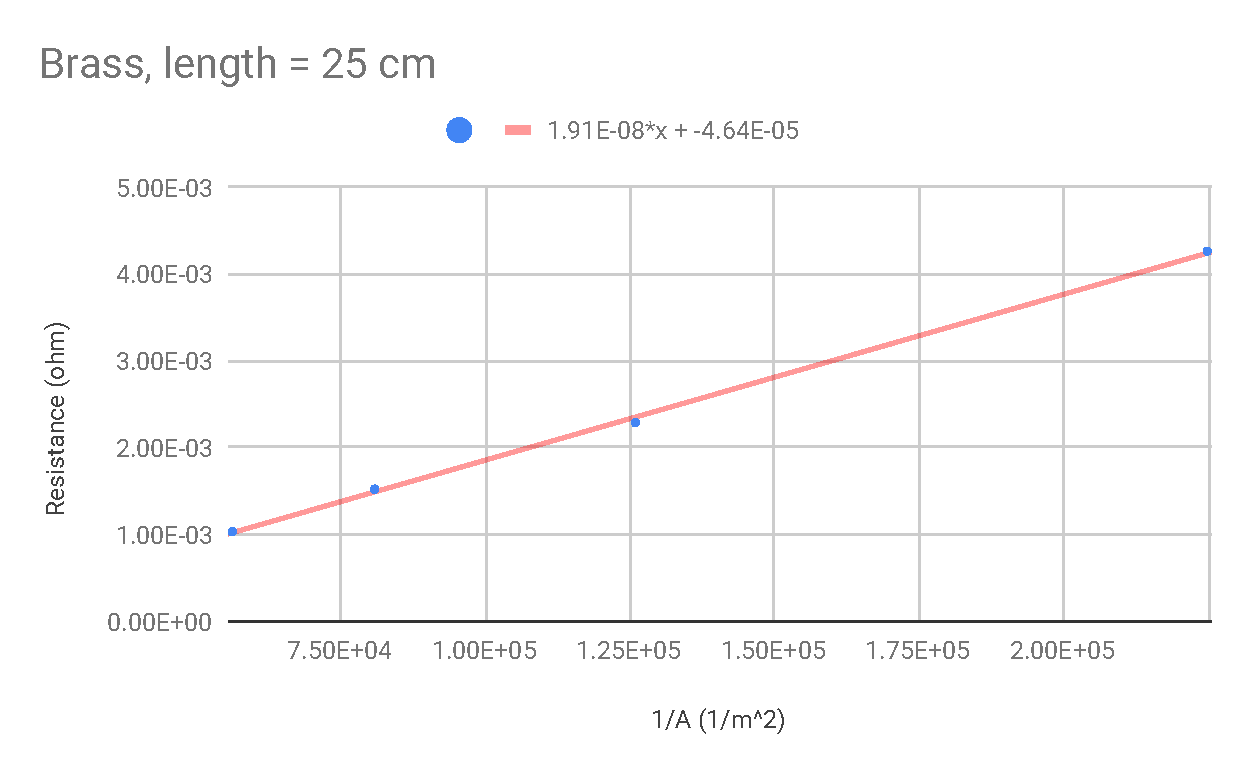
\includegraphics[scale=0.74]{image/02-resistance/25cm.pdf}
	\caption{Brass, $l = 25$ cm}
	\label{figure.02.25cm}
\end{figure}
%

% % Copyright 2018-2019 Melvin Eloy Irizarry-Gelpí
\setcounter{chapter}{2}
\chapter{Serial and Parallel Circuits}
%%%%%%%%%%%%%%%%%%%%%%%%%%%%%%%%%%%%%%%%%%%%%%%%%%%%%%%%%%%%%%%%%%%%%%%%%%%%%%%%
In this experiment you will learn about circuits connected in series or in parallel.
%%%%%%%%%%%%%%%%%%%%%%%%%%%%%%%%%%%%%%%%%%%%%%%%%%%%%%%%%%%%%%%%%%%%%%%%%%%%%%%%
\section{Preliminary}
%%%%%%%%%%%%%%%%%%%%%%%%%%%%%%%%%%%%%%%%%%%%%%%%%%%%%%%%%%%%%%%%%%%%%%%%%%%%%%%%
A \textbf{resistor} is any component in an electric circuit with \textbf{electrical resistance}. Ohm's law is a statement that relates the voltage $V$ across a resistor to the amount of current $I$ leaving (or equivalently, entering) a resistor:
\begin{equation}
	V = R I
\end{equation}
Here, $R$ is the amount of electrical resistance. Solving for $R$ gives
\begin{equation} \label{eq.03.ROhmLaw}
	R = \frac{V}{I}
\end{equation}
For \textbf{ohmic resistors}, the ratio of voltage and current is fixed (i.e. constant) and \textbf{always} gives the same value. This is \textbf{not true} for \textbf{non-ohmic resistors}.

An electric circuit can contain many components that are connected with wires. The electric properties of the circuit will be depend on how these components are connected. You are going to look at two ways of connecting two components in a circuit to a battery: \textbf{series} and \textbf{parallel}.
%%%%%%%%%%%%%%%%%%%%%%%%%%%%%%%%%%%%%%%%%%%%%%%%%%%%%%%%%%%%%%%%%%%%%%%%%%%%%%%%
\subsection{Circuits in Series}
%%%%%%%%%%%%%%%%%%%%%%%%%%%%%%%%%%%%%%%%%%%%%%%%%%%%%%%%%%%%%%%%%%%%%%%%%%%%%%%%
A collection of two resistors in \textbf{series} can be replaced by an \textbf{equivalent resistor} with a resistance given by the sum of the individual resistances:
\begin{equation} \label{eq.03.RSeries}
	R_{\text{eq}} = R_{1} + R_{2}
\end{equation}
When two resistors are connected in \textbf{series} to a battery, the \textbf{current} $I_{0}$ leaving the battery is the same as the \textbf{current} $I_{1}$ leaving resistor 1, and also the same as the \textbf{current} $I_{2}$ leaving resistor 2:
\begin{equation} \label{eq.03.ISeries}
	I_{0} = I_{1} = I_{2}
\end{equation}
When two resistors are connected in \textbf{series} to a battery, the \textbf{voltage} $V_{0}$ across the battery is split between the \textbf{voltage} $V_{1}$ across resistor 1, and the \textbf{voltage} $V_{2}$ across resistor 2:
\begin{equation} \label{eq.03.VSeries}
	V_{0} = \left| V_{1} + V_{2} \right|
\end{equation}
The absolute value is needed because the voltage across each resistor is \textbf{negative} since it correspond to an electric potential drop.
%%%%%%%%%%%%%%%%%%%%%%%%%%%%%%%%%%%%%%%%%%%%%%%%%%%%%%%%%%%%%%%%%%%%%%%%%%%%%%%%
\subsection{Circuits in Parallel}
%%%%%%%%%%%%%%%%%%%%%%%%%%%%%%%%%%%%%%%%%%%%%%%%%%%%%%%%%%%%%%%%%%%%%%%%%%%%%%%%
A collection of two resistors in \textbf{parallel} can be replaced by an \textbf{equivalent resistor} with a resistance that satisfies the relation
\begin{equation}
	\frac{1}{R_{\text{eq}}} = \frac{1}{R_{1}} + \frac{1}{R_{2}}
\end{equation}
Solving for the equivalent resistance gives
\begin{equation} \label{eq.03.RParallel}
	R_{\text{eq}} = \frac{R_{1} R_{2}}{R_{1} + R_{2}}
\end{equation}
When two resistors are connected in \textbf{parallel} to a battery, the \textbf{current} $I_{0}$ leaving the battery is split between the \textbf{current} $I_{1}$ leaving resistor 1, and the \textbf{current} $I_{2}$ leaving resistor 2:
\begin{equation} \label{eq.03.IParallel}
	I_{0} = I_{1} + I_{2}
\end{equation}
When two resistors are connected in \textbf{parallel} to a battery, the \textbf{voltage} $V_{0}$ across the battery is the same as the \textbf{voltage} $V_{1}$ across resistor 1, and also the same as the \textbf{voltage} $V_{2}$ across resistor 2:
\begin{equation} \label{eq.03.VParallel}
	V_{0} = \left| V_{1} \right| = \left| V_{2} \right|
\end{equation}
Again, remember that the voltage across a resistor is negative because it correspond to a drop in electric potential.
%%%%%%%%%%%%%%%%%%%%%%%%%%%%%%%%%%%%%%%%%%%%%%%%%%%%%%%%%%%%%%%%%%%%%%%%%%%%%%%%
\subsection{Power}
%%%%%%%%%%%%%%%%%%%%%%%%%%%%%%%%%%%%%%%%%%%%%%%%%%%%%%%%%%%%%%%%%%%%%%%%%%%%%%%%
The power $P$ input or output of a component in an electric circuit can be found by multiplying the voltage $V$ across that component, and the amount of current $I$ leaving that component:
\begin{equation}
	P = VI
\end{equation}
The SI unit for power is the watt (W). One watt is equivalent to one joule of energy consumed or generated per second:
\begin{equation}
	1 \text{ W} = 1 \text{ J/s}
\end{equation}
%%%%%%%%%%%%%%%%%%%%%%%%%%%%%%%%%%%%%%%%%%%%%%%%%%%%%%%%%%%%%%%%%%%%%%%%%%%%%%%%
\section{Experiment}
%%%%%%%%%%%%%%%%%%%%%%%%%%%%%%%%%%%%%%%%%%%%%%%%%%%%%%%%%%%%%%%%%%%%%%%%%%%%%%%%
There are four experiments. The first two experiments involve using two (ohmic) resistors. The other two experiments use two (non-ohmic) light bulbs.
%%%%%%%%%%%%%%%%%%%%%%%%%%%%%%%%%%%%%%%%%%%%%%%%%%%%%%%%%%%%%%%%%%%%%%%%%%%%%%%%
\subsection{Part 1: Resistors in Series}
%%%%%%%%%%%%%%%%%%%%%%%%%%%%%%%%%%%%%%%%%%%%%%%%%%%%%%%%%%%%%%%%%%%%%%%%%%%%%%%%
In this part, you connect two \textbf{resistors} in \textbf{series} to a battery.
%%%%%%%%%%%%%%%%%%%%%%%%%%%%%%%%%%%%%%%%%%%%%%%%%%%%%%%%%%%%%%%%%%%%%%%%%%%%%%%%
\subsection{Part 2: Resistors in Parallel}
%%%%%%%%%%%%%%%%%%%%%%%%%%%%%%%%%%%%%%%%%%%%%%%%%%%%%%%%%%%%%%%%%%%%%%%%%%%%%%%%
In this part, you connect two \textbf{resistors} in \textbf{parallel} to a battery.
%%%%%%%%%%%%%%%%%%%%%%%%%%%%%%%%%%%%%%%%%%%%%%%%%%%%%%%%%%%%%%%%%%%%%%%%%%%%%%%%
\subsection{Part 3: Light Bulbs in Series}
%%%%%%%%%%%%%%%%%%%%%%%%%%%%%%%%%%%%%%%%%%%%%%%%%%%%%%%%%%%%%%%%%%%%%%%%%%%%%%%%
In this part, you connect two \textbf{light bulbs} in \textbf{series} to a battery.
%%%%%%%%%%%%%%%%%%%%%%%%%%%%%%%%%%%%%%%%%%%%%%%%%%%%%%%%%%%%%%%%%%%%%%%%%%%%%%%%
\subsection{Part 4: Light Bulbs in Parallel}
%%%%%%%%%%%%%%%%%%%%%%%%%%%%%%%%%%%%%%%%%%%%%%%%%%%%%%%%%%%%%%%%%%%%%%%%%%%%%%%%
In this part, you connect two \textbf{light bulbs} in \textbf{parallel} to a battery.
%%%%%%%%%%%%%%%%%%%%%%%%%%%%%%%%%%%%%%%%%%%%%%%%%%%%%%%%%%%%%%%%%%%%%%%%%%%%%%%%
\section{Analysis}
%%%%%%%%%%%%%%%%%%%%%%%%%%%%%%%%%%%%%%%%%%%%%%%%%%%%%%%%%%%%%%%%%%%%%%%%%%%%%%%%
Each run is a measurement of either \textbf{voltage} (electric potential difference between two points) or \textbf{current}. If the voltage and current sensors were zeroed correctly, then the measurement over time should correspond to the measurement of the desired quantity, and no offset or baseline needs to be taken into account. One way to determine a single value is to take the \textbf{time-average}.

Note that each \textbf{voltage measurement has three decimal figures}, and each \textbf{current measurement has four decimal figures}. You should round your time-averaged values appropriately.

In each part there are three components: one battery and two resistors (or two light bulbs). There are \textbf{six quantities} that describe the system:
\begin{itemize}
	\item Time-averaged voltage across the battery: $V_{0}$
	\item Time-averaged voltage across resistor/bulb 1: $V_{1}$
	\item Time-averaged voltage across resistor/bulb 2: $V_{2}$
	\item Time-averaged current leaving the battery: $I_{0}$
	\item Time-averaged current leaving resistor/bulb 1: $I_{1}$
	\item Time-averaged current leaving resistor/bulb 2: $I_{2}$
\end{itemize}
These six quantities satisfy certain mathematical relations. Note that $V_{1}$ and $V_{2}$ are measured to be negative.
%%%%%%%%%%%%%%%%%%%%%%%%%%%%%%%%%%%%%%%%%%%%%%%%%%%%%%%%%%%%%%%%%%%%%%%%%%%%%%%%
\subsection{Part 1: Two Resistors in Series}
%%%%%%%%%%%%%%%%%%%%%%%%%%%%%%%%%%%%%%%%%%%%%%%%%%%%%%%%%%%%%%%%%%%%%%%%%%%%%%%%
For the two \textbf{resistors in series}, you find the time average for all six quantities above and fill a table similar to Table \ref{table.03.resistors.series}.

You should check that relations (\ref{eq.03.ISeries}) and (\ref{eq.03.VSeries}) hold true. The percent difference between the labeled resistance and the prediction (\ref{eq.03.ROhmLaw}) from Ohm's law should be very small. The resistance of the battery should be very close to the series equivalent resistance in (\ref{eq.03.RSeries}).
%%%%%%%%%%%%%%%%%%%%%%%%%%%%%%%%%%%%%%%%%%%%%%%%%%%%%%%%%%%%%%%%%%%%%%%%%%%%%%%%
\subsection{Part 2: Two Resistors in Parallel}
%%%%%%%%%%%%%%%%%%%%%%%%%%%%%%%%%%%%%%%%%%%%%%%%%%%%%%%%%%%%%%%%%%%%%%%%%%%%%%%%
For the two \textbf{resistors in parallel}, you find the time average for all six quantities above and fill a table similar to Table \ref{table.03.resistors.parallel}.

You should check that relations (\ref{eq.03.IParallel}) and (\ref{eq.03.VParallel}) hold true. The percent difference between the labeled resistance and the prediction (\ref{eq.03.ROhmLaw}) from Ohm's law should be very small. The resistance of the battery should be very close to the parallel equivalent resistance in (\ref{eq.03.RParallel}).
%%%%%%%%%%%%%%%%%%%%%%%%%%%%%%%%%%%%%%%%%%%%%%%%%%%%%%%%%%%%%%%%%%%%%%%%%%%%%%%%
\subsection{Part 3: Two Light Bulbs in Series}
%%%%%%%%%%%%%%%%%%%%%%%%%%%%%%%%%%%%%%%%%%%%%%%%%%%%%%%%%%%%%%%%%%%%%%%%%%%%%%%%
For two \textbf{light bulbs in series}, you can find the time average for all six quantities mentioned above, and fill a table similar to Table \ref{table.03.bulbs.series}. Note that the fourth column consist of the ratio of voltage and current for each component. This is a quantity with units of resistance (ohms) but it does not correspond to the actual resistance of the light bulbs. As you will find, the light bulbs are not ohmic, and thus the ratio of the voltage across the light bulb and the current leaving the light bulb is not constant. However, you should find that the relations (\ref{eq.03.ISeries}) and (\ref{eq.03.VSeries}) again hold.
%%%%%%%%%%%%%%%%%%%%%%%%%%%%%%%%%%%%%%%%%%%%%%%%%%%%%%%%%%%%%%%%%%%%%%%%%%%%%%%%
\subsection{Part 4: Two Light Bulbs in Parallel}
%%%%%%%%%%%%%%%%%%%%%%%%%%%%%%%%%%%%%%%%%%%%%%%%%%%%%%%%%%%%%%%%%%%%%%%%%%%%%%%%
For two \textbf{light bulbs in parallel}, you can find the time average for all six quantities mentioned above, and table similar to Table \ref{table.03.bulbs.parallel}. Note that the fourth column consist of the ratio of voltage and current for each component. You can verify that the light bulbs are not ohmic by showing that the values in the fourth column in Tables \ref{table.03.bulbs.series} and \ref{table.03.bulbs.parallel} are very different. However, you should find that the relations (\ref{eq.03.IParallel}) and (\ref{eq.03.VParallel}) again hold.
%%%%%%%%%%%%%%%%%%%%%%%%%%%%%%%%%%%%%%%%%%%%%%%%%%%%%%%%%%%%%%%%%%%%%%%%%%%%%%%%
\section{My Data}
%%%%%%%%%%%%%%%%%%%%%%%%%%%%%%%%%%%%%%%%%%%%%%%%%%%%%%%%%%%%%%%%%%%%%%%%%%%%%%%%
For parts 1 and 2, I used \textbf{three} resistors, instead of two. The resistances are given by
\begin{align}
	R_{1} = 10 \text{ ohm} && R_{2} = 51 \text{ ohm} && R_{3} = 68 \text{ ohm}
\end{align}
The equivalent resistance in \textbf{series} with three resistors is given by
\begin{equation}
	R_{\text{eq}} = R_{1} + R_{2} + R_{3}
\end{equation}
In parallel, the equivalent resistant satisfies the following relation:
\begin{equation}
	\frac{1}{R_{\text{eq}}} = \frac{1}{R_{1}} + \frac{1}{R_{2}} + \frac{1}{R_{3}}
\end{equation}
Solving for the equivalent resistance in \textbf{parallel} gives
\begin{equation}
	R_{\text{eq}} = \frac{R_{1} R_{2} R_{3}}{R_{1} R_{2} + R_{1} R_{3} + R_{2} R_{3}}
\end{equation}
As you can see from my spreadsheet, the results are in good agreement with expectations.
%%%%%%%%%%%%%%%%%%%%%%%%%%%%%%%%%%%%%%%%%%%%%%%%%%%%%%%%%%%%%%%%%%%%%%%%%%%%%%%%
\subsection{Part 1: Three Resistors in Series}
%%%%%%%%%%%%%%%%%%%%%%%%%%%%%%%%%%%%%%%%%%%%%%%%%%%%%%%%%%%%%%%%%%%%%%%%%%%%%%%%
Table \ref{table.03.3resistors.series} has the results for three resistors in series. You can check that the values for the current in the third column are all very close. Indeed,
\begin{equation}
	I_{0} \approx I_{1} \approx I_{2} \approx I_{3}
\end{equation}
This is the three-resistor analog of (\ref{eq.03.ISeries}). Also, you can check that
\begin{equation}
	| V_{1} + V_{2} + V_{3} | = 3.075 \text{ V}
\end{equation}
which is very close to the value of $V_{0}$ (the voltage across the battery). This is the three-resistor analog of (\ref{eq.03.VSeries}).

The last column in Table \ref{table.03.3resistors.series} contains the power generated/consumed by the corresponding component. As you can see, the rate of energy generation for the battery is very close to the sum of the rate of consumption for each resistor. Note that, in \textbf{series}, the resistor with the \textbf{largest} resistance consumes the most energy.
%%%%%%%%%%%%%%%%%%%%%%%%%%%%%%%%%%%%%%%%%%%%%%%%%%%%%%%%%%%%%%%%%%%%%%%%%%%%%%%%
\subsection{Part 2: Three Resistors in Parallel}
%%%%%%%%%%%%%%%%%%%%%%%%%%%%%%%%%%%%%%%%%%%%%%%%%%%%%%%%%%%%%%%%%%%%%%%%%%%%%%%%
Table \ref{table.03.3resistors.parallel} has the results for three resistors in parallel. You can check that, ignoring the signs, the values for the voltage in the second column are all very close. Indeed,
\begin{equation}
	V_{0} \approx |V_{1}| \approx |V_{2}| \approx |V_{3}|
\end{equation}
This is the three-resistor analog of (\ref{eq.03.VParallel}). Also, you can check that
\begin{equation}
	I_{1} + I_{2} + I_{3}  = 0.3532 \text{ A}
\end{equation}
which is very close to the value of $I_{0}$ (the current leaving the battery). This is the three-resistor analog of (\ref{eq.03.IParallel}).

The last column in Table \ref{table.03.3resistors.parallel} contains the power generated/consumed by the corresponding component. As you can see, the rate of energy generation for the battery is very close to the sum of the rate of consumption for each resistor. Note that, in \textbf{parallel}, the resistor with the \textbf{smallest} resistance consumes the most energy.

One last thing about resistors: proof that they \textbf{are ohmic} (at least for the amount of voltage and current that we used) is that the values in the fourth column in Tables \ref{table.03.3resistors.series} and \ref{table.03.3resistors.parallel} are consistent (except for the first value, because it corresponds to the equivalent resistance). That is, it does not matter if they are connected in series or parallel, the amount of current going through the resistor is proportional to the amount of voltage across the resistor.
%%%%%%%%%%%%%%%%%%%%%%%%%%%%%%%%%%%%%%%%%%%%%%%%%%%%%%%%%%%%%%%%%%%%%%%%%%%%%%%%
\subsection{Part 3: Two Light Bulbs in Series}
%%%%%%%%%%%%%%%%%%%%%%%%%%%%%%%%%%%%%%%%%%%%%%%%%%%%%%%%%%%%%%%%%%%%%%%%%%%%%%%%
The six runs in the text file \texttt{bulbs-serial.txt} are for two light bulbs connected in series.
\begin{itemize}
	\item Run 1: measurement of voltage across battery ($V_{0}$).
	\item Run 2: measurement of voltage across long light bulb ($V_{L}$).
	\item Run 3: measurement of voltage across round light bulb ($V_{R}$).
	\item Run 4: measurement of current leaving battery ($I_{0}$).
	\item Run 5: measurement of current leaving long light bulb ($I_{L}$).
	\item Run 6: measurement of current leaving round light bulb ($I_{R}$).
\end{itemize}
The \textbf{long} light bulb is connected \textbf{first}, and the \textbf{round} light bulb is connected \textbf{second}.
%%%%%%%%%%%%%%%%%%%%%%%%%%%%%%%%%%%%%%%%%%%%%%%%%%%%%%%%%%%%%%%%%%%%%%%%%%%%%%%%
\subsection{Part 4: Two Light Bulbs in Parallel}
%%%%%%%%%%%%%%%%%%%%%%%%%%%%%%%%%%%%%%%%%%%%%%%%%%%%%%%%%%%%%%%%%%%%%%%%%%%%%%%%
The six runs in the text file \texttt{bulbs-parallel.txt} are for two light bulbs connected in parallel.
\begin{itemize}
	\item Run 1: measurement of voltage across battery ($V_{0}$).
	\item Run 2: measurement of voltage across long light bulb ($V_{L}$).
	\item Run 3: measurement of voltage across round light bulb ($V_{R}$).
	\item Run 4: measurement of current leaving battery ($I_{0}$).
	\item Run 5: measurement of current leaving long light bulb ($I_{L}$).
	\item Run 6: measurement of current leaving round light bulb ($I_{R}$).
\end{itemize}
%%%%%%%%%%%%%%%%%%%%%%%%%%%%%%%%%%%%%%%%%%%%%%%%%%%%%%%%%%%%%%%%%%%%%%%%%%%%%%%%
\section{Your Data}
%%%%%%%%%%%%%%%%%%%%%%%%%%%%%%%%%%%%%%%%%%%%%%%%%%%%%%%%%%%%%%%%%%%%%%%%%%%%%%%%
If your data for resistors in series and/or parallel is not good, let me know via email and I will make data available to you.
%%%%%%%%%%%%%%%%%%%%%%%%%%%%%%%%%%%%%%%%%%%%%%%%%%%%%%%%%%%%%%%%%%%%%%%%%%%%%%%%
\newpage
\section{Your Lab Report}
%%%%%%%%%%%%%%%%%%%%%%%%%%%%%%%%%%%%%%%%%%%%%%%%%%%%%%%%%%%%%%%%%%%%%%%%%%%%%%%%
In your lab report you should include:
\begin{enumerate}
	\item One table like Table \ref{table.03.resistors.series} for two resistors in series.
	\item One table like Table \ref{table.03.resistors.parallel} for two resistors in parallel.
	\item One table like Table \ref{table.03.bulbs.series} for two light bulbs in series.
	\item One table like Table \ref{table.03.bulbs.parallel} for two light bulbs in parallel.
\end{enumerate}
You should also:
\begin{enumerate}
	\item Verify that equations (\ref{eq.03.ISeries}) and (\ref{eq.03.VSeries}) hold for two resistors, and also for two light bulbs, connected in series.
	\item Verify that the voltage across the battery divided by the current leaving the battery is close to (\ref{eq.03.RSeries}) for two resistors in series.
	\item Verify that equations (\ref{eq.03.IParallel}) and (\ref{eq.03.VParallel}) hold for two resistors, and also for two light bulbs, connected in parallel.
	\item Verify that the voltage across the battery divided by the current leaving the battery is close to (\ref{eq.03.RParallel}) for two resistors in parallel.
	\item Confirm that the long light bulb is non-ohmic by comparing the ratio of the voltage and the current $V_{1} / I_{1}$ in series and in parallel.
	\item Confirm that the round light bulb is non-ohmic by comparing the ratio of the voltage and the current $V_{2} / I_{2}$ in series and in parallel.
	\item Find which resistor consumes more power when two resistors are connected in series.
	\item Find which resistor consumes more power when two resistors are connected in parallel.
	\item Find which light bulb consumes more power when two light bulbs are connected in series.
	\item Find which light bulb consumes more power when two light bulbs are connected in parallel.
\end{enumerate}
%%%%%%%%%%%%%%%%%%%%%%%%%%%%%%%%%%%%%%%%%%%%%%%%%%%%%%%%%%%%%%%%%%%%%%%%%%%%%%%%
\newpage
\section{Tables}
%%%%%%%%%%%%%%%%%%%%%%%%%%%%%%%%%%%%%%%%%%%%%%%%%%%%%%%%%%%%%%%%%%%%%%%%%%%%%%%%
\begin{table}[ht]
	\begin{center}
		\begin{tabular}{|l|r|r|r|r|r|r|}
			\hline
			Name & $V$ (V) & $I$ (A) & $V/I$ (ohm) & Expected $R$ (ohm) & P.D. (\%) & $V I$ (W) \\
			\hline
			Battery & $V_{0}$ & $I_{0}$ & $V_{0} / I_{0}$ & $R_{1} + R_{2}$ & ??? & $V_{0} I_{0}$ \\
			Resistor 1 & $V_{1}$ & $I_{1}$ & $V_{1} / I_{1}$ & $R_{1}$ & ??? & $V_{1} I_{1}$ \\
			Resistor 2 & $V_{2}$ & $I_{2}$ & $V_{2} / I_{2}$ & $R_{2}$ & ??? & $V_{2} I_{2}$ \\
			\hline
		\end{tabular}
	\end{center}
	\caption{Time-averages and resistance for two resistors in series.}
	\label{table.03.resistors.series}
\end{table}
%%%%%%%%%%%%%%%%%%%%%%%%%%%%%%%%%%%%%%%%%%%%%%%%%%%%%%%%%%%%%%%%%%%%%%%%%%%%%%%%
\begin{table}[ht]
	\begin{center}
		\begin{tabular}{|l|r|r|r|r|r|r|}
			\hline
			Name & $V$ (V) & $I$ (A) & $V/I$ (ohm) & Expected $R$ (ohm) & P.D. (\%) & $V I$ (W) \\
			\hline
			Battery & $V_{0}$ & $I_{0}$ & $V_{0} / I_{0}$ & $R_{1} R_{2} / (R_{1} + R_{2})$ & ??? & $V_{0} I_{0}$ \\
			Resistor 1 & $V_{1}$ & $I_{1}$ & $V_{1} / I_{1}$ & $R_{1}$ & ??? & $V_{1} I_{1}$ \\
			Resistor 2 & $V_{2}$ & $I_{2}$ & $V_{2} / I_{2}$ & $R_{2}$ & ??? & $V_{2} I_{2}$ \\
			\hline
		\end{tabular}
	\end{center}
	\caption{Time-averages and resistance for two resistors in parallel.}
	\label{table.03.resistors.parallel}
\end{table}
%%%%%%%%%%%%%%%%%%%%%%%%%%%%%%%%%%%%%%%%%%%%%%%%%%%%%%%%%%%%%%%%%%%%%%%%%%%%%%%%
\begin{table}[ht]
	\begin{center}
		\begin{tabular}{|l|r|r|r|r|}
			\hline
			Name & $V$ (V) & $I$ (A) & $V/I$ (ohm) & $V I$ (W) \\
			\hline
			Battery & $V_{0}$ & $I_{0}$ & $V_{0} / I_{0}$ & $V_{0} I_{0}$ \\
			Long Bulb & $V_{L}$ & $I_{L}$ & $V_{L} / I_{L}$ & $V_{L} I_{L}$ \\
			Round Bulb & $V_{R}$ & $I_{R}$ & $V_{R} / I_{R}$ & $V_{R} I_{R}$ \\
			\hline
		\end{tabular}
	\end{center}
	\caption{Time-averages and power for two light bulbs in series.}
	\label{table.03.bulbs.series}
\end{table}
%%%%%%%%%%%%%%%%%%%%%%%%%%%%%%%%%%%%%%%%%%%%%%%%%%%%%%%%%%%%%%%%%%%%%%%%%%%%%%%%
\begin{table}[ht]
	\begin{center}
		\begin{tabular}{|l|r|r|r|r|}
			\hline
			Name & $V$ (V) & $I$ (A) & $V/I$ (ohm) & $V I$ (W) \\
			\hline
			Battery & $V_{0}$ & $I_{0}$ & $V_{0} / I_{0}$ & $V_{0} I_{0}$ \\
			Long Bulb & $V_{L}$ & $I_{L}$ & $V_{L} / I_{L}$ & $V_{L} I_{L}$ \\
			Round Bulb & $V_{R}$ & $I_{R}$ & $V_{R} / I_{R}$ & $V_{R} I_{R}$ \\
			\hline
		\end{tabular}
	\end{center}
	\caption{Time-averages and power for two light bulbs in parallel.}
	\label{table.03.bulbs.parallel}
\end{table}
%%%%%%%%%%%%%%%%%%%%%%%%%%%%%%%%%%%%%%%%%%%%%%%%%%%%%%%%%%%%%%%%%%%%%%%%%%%%%%%%
\begin{table}[ht]
	\begin{center}
		\begin{tabular}{|l|r|r|r|r|r|r|}
			\hline
			Name & $V$ (V) & $I$ (A) & $V/I$ (ohm) & Expected $R$ (ohm) & P.D. (\%) & $V I$ (W) \\
			\hline
			Battery & 4.430 & 0.0346 & 128.05 & 129 & $-0.73$ & 0.15 \\
			Resistor 1 & $-0.338$ & 0.0346 & 9.76 & 10 & $-2.36$ & $-0.01$ \\
			Resistor 2 & $-1.757$ & 0.0347 & 50.70 & 51 & $-0.58$ & $-0.06$ \\
			Resistor 3 & $-2.345$ & 0.0347 & 67.68 & 68 & $-0.46$ & $-0.08$ \\
			\hline
		\end{tabular}
	\end{center}
	\caption{Time-averages and resistance for three resistors in series.}
	\label{table.03.3resistors.series}
\end{table}
%%%%%%%%%%%%%%%%%%%%%%%%%%%%%%%%%%%%%%%%%%%%%%%%%%%%%%%%%%%%%%%%%%%%%%%%%%%%%%%%
\begin{table}[ht]
	\begin{center}
		\begin{tabular}{|l|r|r|r|r|r|r|}
			\hline
			Name & $V$ (V) & $I$ (A) & $V/I$ (ohm) & Expected $R$ (ohm) & P.D. (\%) & $V I$ (W) \\
			\hline
			Battery & 3.731 & 0.4904 & 7.61 & 7.45 & 2.20 & 1.83 \\
			Resistor 1 & $-3.707$ & 0.3722 & 9.96 & 10 & $-0.39$ & $-1.38$ \\
			Resistor 2 & $-3.736$ & 0.0739 & 50.55 & 51 & $-0.88$ & $-0.28$ \\
			Resistor 3 & $-3.734$ & 0.0554 & 67.37 & 68 & $-0.92$ & $-0.21$ \\
			\hline
		\end{tabular}
	\end{center}
	\caption{Time-averages and resistance for three resistors in parallel.}
	\label{table.03.3resistors.parallel}
\end{table}
%%%%%%%%%%%%%%%%%%%%%%%%%%%%%%%%%%%%%%%%%%%%%%%%%%%%%%%%%%%%%%%%%%%%%%%%%%%%%%%%
\FloatBarrier
\newpage
\section{Figures}
%%%%%%%%%%%%%%%%%%%%%%%%%%%%%%%%%%%%%%%%%%%%%%%%%%%%%%%%%%%%%%%%%%%%%%%%%%%%%%%%
\begin{figure}[ht]
	\centering
	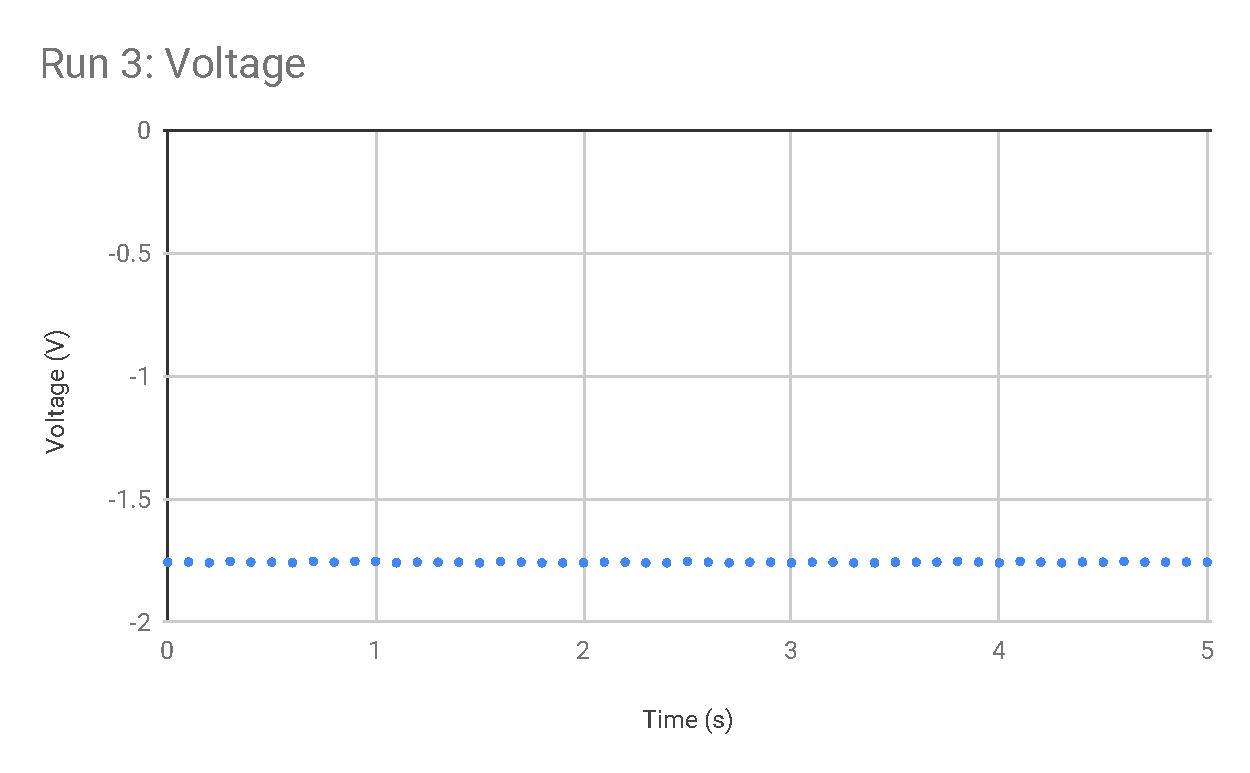
\includegraphics[scale=0.74]{image/03-serial-parallel/resistor-V.pdf}
	\caption{Voltage across ohmic resistor}
	\label{figure.03.resistor.v}
\end{figure}
%%%%%%%%%%%%%%%%%%%%%%%%%%%%%%%%%%%%%%%%%%%%%%%%%%%%%%%%%%%%%%%%%%%%%%%%%%%%%%%%
\begin{figure}[ht]
	\centering
	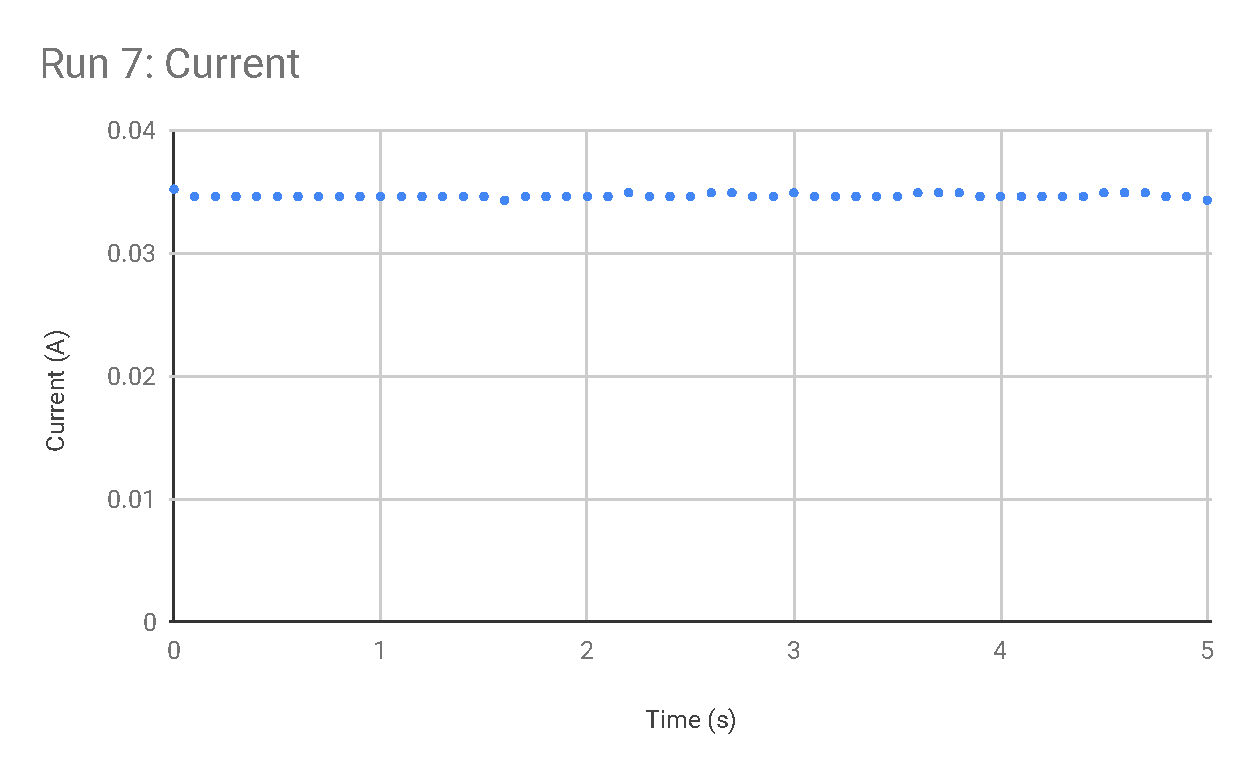
\includegraphics[scale=0.74]{image/03-serial-parallel/resistor-I.pdf}
	\caption{Current through ohmic resistor}
	\label{figure.03.resistor.i}
\end{figure}
%%%%%%%%%%%%%%%%%%%%%%%%%%%%%%%%%%%%%%%%%%%%%%%%%%%%%%%%%%%%%%%%%%%%%%%%%%%%%%%%
\begin{figure}[ht]
	\centering
	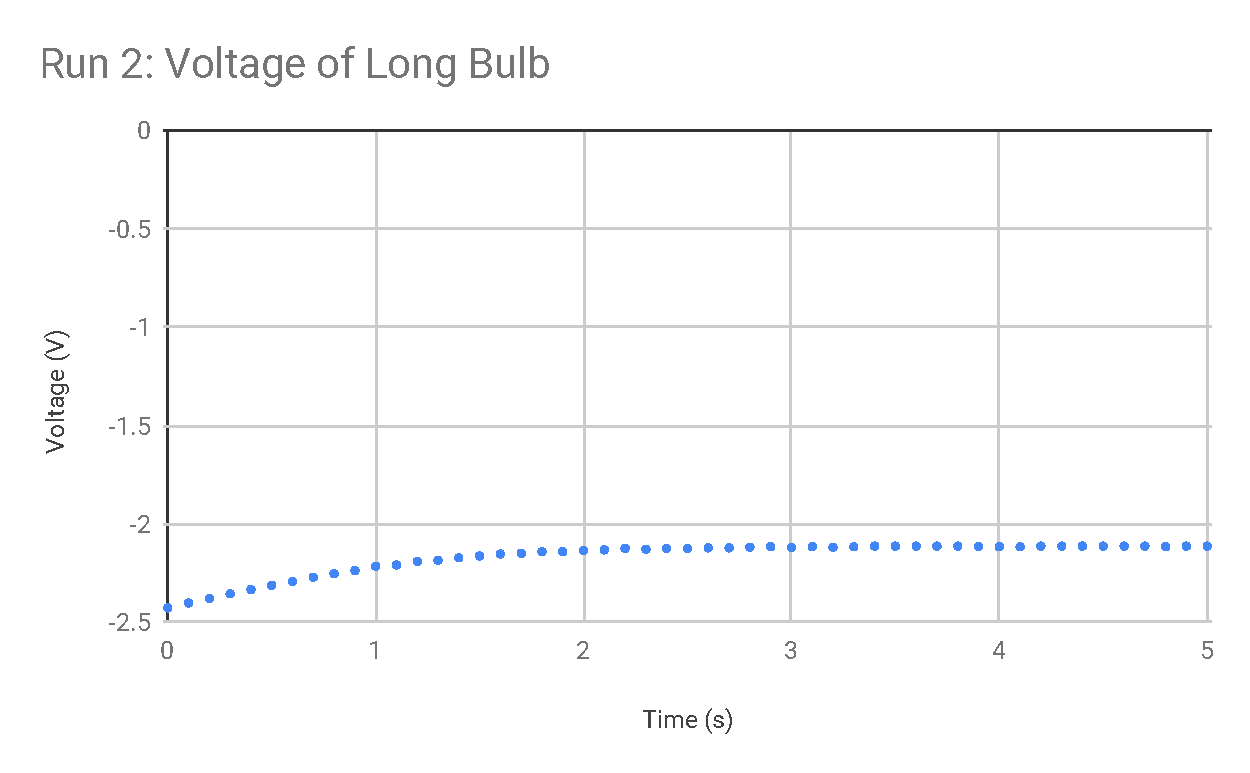
\includegraphics[scale=0.74]{image/03-serial-parallel/bulb-V.pdf}
	\caption{Voltage across non-ohmic light bulb}
	\label{figure.03.bulb.v}
\end{figure}
%%%%%%%%%%%%%%%%%%%%%%%%%%%%%%%%%%%%%%%%%%%%%%%%%%%%%%%%%%%%%%%%%%%%%%%%%%%%%%%%
\begin{figure}[ht]
	\centering
	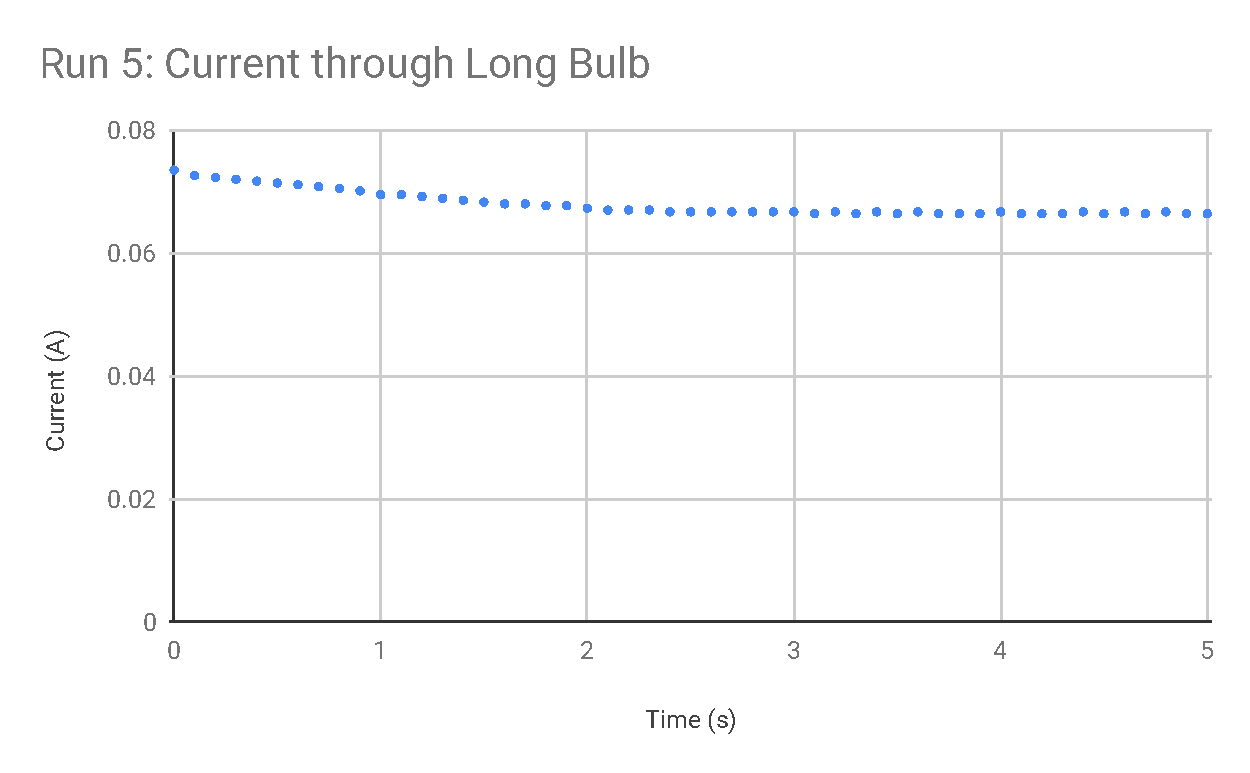
\includegraphics[scale=0.74]{image/03-serial-parallel/bulb-I.pdf}
	\caption{Current through non-ohmic light bulb}
	\label{figure.03.bulb.i}
\end{figure}
% % Copyright 2018-2020 Melvin Eloy Irizarry-Gelpí
\setcounter{chapter}{3}
\chapter{Faraday's Law}
%
In this experiment you will learn about Faraday's law of induction and a relationship between electric and magnetic phenomena.
%
\section{Preliminary}
%
Faraday's law of induction is a statement relating one \textbf{electric} phenomenon to one \textbf{magnetic} phenomenon. It states that a certain amount of voltage $\mathcal{E}$ is equal to the negative rate of change of the magnetic flux $\Phi_{B}$ with time:
\begin{equation}
	\mathcal{E} = -\frac{\Delta \Phi_{B}}{\Delta t}
	\label{eq.04.faradays.law}
\end{equation}
Here $\mathcal{E}$ is known as the \textbf{electro-motive force} or EMF. Although ``force'' is part of its name, an EMF quantity has nothing to do with force (which is measured in newtons): an EMF quantity has units of volts.

The \textbf{magnetic flux} is defined as the product of the amount of \textbf{magnetic field} $B$ and the amount of \textbf{area} $a$ in a surface where the magnetic field lines pass through:
\begin{equation}
	\Phi_{B} = B a
\end{equation}
The \textbf{SI unit} for magnetic field is the tesla (T). The \textbf{SI unit} for area is the square meter (m$^{2}$). Thus, magnetic flux is measured in units of T{ }\textperiodcentered{ }m\textsuperscript{2}.

A non-zero EMF $\mathcal{E}$ requires the magnetic flux $\Phi_{B}$ to change with time. In this experiment you are going to keep the \textbf{area fixed} and let the \textbf{magnetic field change with time}. In this setting, the rate of change of the magnetic flux with time is proportional to the rate of change of the magnetic field with time:
\begin{align}
	\Phi_{B} = B a && \Longrightarrow && \frac{\Delta \Phi_{B}}{\Delta t} = \left(\frac{\Delta B}{\Delta t}\right) a
	\label{eq.04.flux.rate}
\end{align}
The rate of change of magnetic flux is measured in units of T{ }\textperiodcentered{ }m\textsuperscript{2}/s. But according to Faraday's law, these units are the same as the units for EMF (volts), so you must have the equivalence:
\begin{equation}
	1 \ \text{V} = 1 \ \text{T{ }\textperiodcentered{ }m\textsuperscript{2}/s}
\end{equation}
This allows you to define the tesla unit in terms of volts, meters, and seconds:
\begin{equation}
	1 \ \text{T} = 1 \ \text{V{ }\textperiodcentered{ }s/m\textsuperscript{2}}
\end{equation}

Wires with electric current produce magnetic fields. You are going to use a particular wire called a \textbf{solenoid coil}. The \textbf{magnetic field} $B$ inside the cylindrical space of a solenoid coil is (almost) uniform and the amount of field is directly proportional to the amount of current $I$ flowing through the coil:
\begin{equation}
	B = \left(\frac{\mu_{0} N_{1}}{L}\right) I
	\label{eq.04.B.coil}
\end{equation}
Here
\begin{itemize}
	\item $B$ is the amount of \textbf{magnetic field} (unit: T)
	\item $\mu_{0} = 4 \pi \times 10^{-7}$ T{ }\textperiodcentered{ }m/A  is a universal physical \textbf{constant}
	\item $N_{1}$ is the \textbf{number of turns} in the (primary) coil (no units)
	\item $L$ is the \textbf{length} of the (primary) coil (unit: m)
	\item $I$ is the amount of \textbf{electric current} through the (primary) coil (unit: A)
\end{itemize}
For a given coil you are going to keep the \textbf{number of turns fixed}, and the \textbf{length fixed}, but you are going to use a \textbf{current that changes with time}. In this case, the rate of change of the magnetic field with time is proportional to the rate of change of the current with time:
\begin{align}
	B = \left(\frac{\mu_{0} N_{1}}{L}\right) I && \Longrightarrow && \frac{\Delta B}{\Delta t} = \left( \frac{\mu_{0} N_{1}}{L} \right) \frac{\Delta I}{\Delta t}
	\label{eq.04.B.rate}
\end{align}
Using (\ref{eq.04.B.rate}) in (\ref{eq.04.flux.rate}) gives
\begin{equation}
	\frac{\Delta \Phi_{B}}{\Delta t} = \left( \frac{\mu_{0} N_{1} a}{L} \right) \frac{\Delta I}{\Delta t}
\end{equation}
Thus, according to Faraday's Law, for a solenoid coil you should have
\begin{equation}
	\mathcal{E} = -\left( \frac{\mu_{0} N_{1} a}{L} \right) \frac{\Delta I}{\Delta t}
	\label{eq.04.emf.solenoid}
\end{equation}
That is, the EMF associated with the area $a$ is proportional to the rate of change of the electric current with respect to time.
%
\section{Experiment}
%
The overall goal of the experiment is to check that the EMF behaves like the rate of change of the electric current. To do this you need to measure the EMF voltage and the current. From the current you can estimate the rate of change and confirm that it agrees with the EMF data. You are going to look at \textbf{five ways for the current to change with time}:
\begin{enumerate}
	\item \textbf{Sinusoidal}: current will change according to a \textbf{sine or cosine} profile.
	\item \textbf{Square}: current will stay almost \textbf{constant}, but the \textbf{sign changes}.
	\item \textbf{Triangular}: current will increase \textbf{linearly}, then decrease \textbf{linearly}.
	\item \textbf{Ramp-up}: current will \textbf{increase linearly}, then \textbf{abruptly drop} to its base value.
	\item \textbf{Ramp-down}: current will \textbf{decrease linearly}, then \textbf{abruptly rise} to its base value.
\end{enumerate}
Each profile for the current leads to different results for the induced EMF.
%
\subsection{Rates of Change}
%
Here is a quick review of rates of change.
%
\subsubsection{Constant Quantity}
%
The rate of change of a \textbf{constant quantity} is \textbf{zero}. That is, if the quantity is not changing, then no amount is being gained or lost.
%
\subsubsection{Quantity Increasing Linearly}
%
The rate of change of a \textbf{quantity that increases linearly with time} is a \textbf{constant}. Increasing linearly is the same as being proportional to time. This means that the slope is constant. Moreover, since the quantity is increasing, the \textbf{slope is positive}.
%
\subsubsection{Quantity Decreasing Linearly}
%
The rate of change of a \textbf{quantity that decreases linearly with time} is a \textbf{constant}. Decreasing linearly is the same as being proportional to time. This means that the slope is constant. However, since the quantity is decreasing, the \textbf{slope is negative}.
%
\subsubsection{Sinusoidal Change}
%
The rate of change of the \textbf{sine function} is a cosine function:
\begin{equation}
	\frac{\Delta \sin(t)}{\Delta t} = \cos(t)
\end{equation}
Similarly, the rate of change of the \textbf{cosine function} is proportional to a sine function:
\begin{equation}
	\frac{\Delta \cos(t)}{\Delta t} = -\sin(t)
\end{equation}
Here the sign is not important. What is important is to remember that sine and cosine are very similar functions and that a cosine is the same as a sine function shifted by 90 deg (or $\pi/2$ rad):
\begin{align}
	\cos(t) = \sin(t + 90\text{\textdegree}), && \sin(t) = \cos(t - 90\text{\textdegree})
\end{align}
Thus, if the quantity is sinusoidal, then the rate of change will also be sinusoidal but shifted by 90 deg. In particular, when $\sin(t)$ is at a peak or valley, then $\cos(t)$ is crossing the horizontal axis (i.e. close to zero), and when $\sin(t)$ is crossing the horizontal axis (i.e. close to zero), then $\cos(t)$ is either at a valley or a peak.
%
\subsection{Solenoid Coils}
%
You are going to use two solenoid coils. The smaller one fits inside the larger one. The smaller one is called the \textbf{secondary coil}. This is the coil used to measure the EMF value. The larger coil is called the \textbf{primary coil}. This coil is the one with the current and the one that produces the magnetic field.

The \textbf{primary coil} has a length of 10 cm and 3300 turns. Thus,
\begin{align}
	L = 10 \ \text{cm} = 0.1 \ \text{m,} && N_{1} = 3300
\end{align}
The \textbf{secondary coil} has 150 turns and an outer diameter of 1.8 cm. The inner diameter I measured it to be close to 1.1 cm. The average of these two diameters correspond to the diameter half-way between these two. This average is 1.45 cm. Since the wire was very thick, I think it is more accurate to use the average of the diameters to calculate the area of each loop. Thus,
\begin{align}
	d = 1.45 \ \text{cm} = 0.0145 \ \text{m,} && N_{2} = 150
\end{align}
The area enclosed by a circular loop with diameter $d$ is given by
\begin{equation}
	a_{\text{loop}} = \frac{1}{4} \pi d^{2} = \frac{1}{4} \pi \left(0.0145 \ \text{m}\right)^2 = 1.65 \times 10^{-4} \ \text{m\textsuperscript{2}}
\end{equation}
This is the amount of \textbf{area-per-loop} in the secondary coil. The \textbf{total amount of area} $a$ is the area-per-loop $a_{\text{loop}}$ multiplied by the number of loops $N_{2}$ in the secondary coil:
\begin{equation}
	a = N_{2} a_{\text{loop}} = 150 \times \left(1.65 \times 10^{-4} \ \text{m\textsuperscript{2}}\right) = 2.48 \times 10^{-2} \ \text{m\textsuperscript{2}}
\end{equation}
This is the amount of area that you will use to measure the magnetic flux.
%
\section{Analysis}
%
According to (\ref{eq.04.emf.solenoid}), the amount of EMF is directly proportional to the amount of rate of change of the current with time. The constant of proportionality is
\begin{equation}
	\frac{\mu_{0} N_{1} a}{L} = 1.03 \times 10^{-3} \ \text{V{ }\textperiodcentered{ }s/A} = 1.03 \ \text{mV{ }\textperiodcentered{ }s/A}
	\label{eq.04.slope}
\end{equation}
This is the expected value. In principle, if you could chart $\mathcal{E}$ versus $\Delta I / \Delta t$, the slope should correspond to the negative of this value. You can only do this for the triangular current profile.
%
\subsection{Sinusoidal Current Profile}
%
For the sinusoidal current profile, one way to check the validity of Faraday's law is by comparing the fit parameters for a sinusoidal fit for both current and voltage. A ``sine'' sinusoidal fit for the current is of the form
\begin{equation}
	I(t) = A \sin\left(B t + C\right) + D
\end{equation}
Note that
\begin{itemize}
	\item The current amplitude $A$ has units of amps (A)
	\item The current angular frequency $B$ has units of radians-per-second (rad/s)
	\item The current angular shift $C$ has units of radians (rad)
	\item The current shift $D$ has units of amps (A)
\end{itemize}
A ``cosine'' sinusoidal fit for the EMF is of the form
\begin{equation}
	\mathcal{E}(t) = W \cos\left(X t + Y\right) + Z
\end{equation}
Note that
\begin{itemize}
	\item The EMF amplitude $W$ has units of volts (V)
	\item The EMF angular frequency $X$ has units of radians-per-second (rad/s)
	\item The EMF angular shift $Y$ has units of radians (rad)
	\item The EMF shift $Z$ has units of volts (V)
\end{itemize}
If the sensors were zeroed correctly, you should find that both $D$ and $Z$ are close to \textbf{zero}, and can be neglected. There are three simple checks:
\begin{enumerate}
	\item The value of $W$ should be very close to
	\begin{equation}
		A B \left(\frac{\mu_{0} N_{1} a}{L}\right)
	\end{equation}
	\item The value of $B$ should be very close to the value of $X$.
	\item The value of $\vert C - Y \vert$ should be very close to $\pi$.
\end{enumerate}
Another check, similar to what you did for simple harmonic motion, is to make a \textbf{phase space} chart, with EMF voltage in the vertical axis, and current in the horizontal axis. Just like for the mass on the spring, the phase space chart should have the \textbf{shape of an ellipse}.
%
\subsection{Square Current Profile}
%
Since the square current profile consists of segments where the current is almost constant, the rate of change of the current should be almost zero. This will result in an EMF value that is also almost zero. You can confirm this by examining a scatter chart with EMF voltage on the vertical axis and time in the horizontal axis.
%
\subsection{Triangular Current Profile}
%
For the triangular current, the chart of current versus time has regions of increasing current and regions of decreasing current. In the same time regions, the EMF voltage is approximately constant but either positive or negative.

You can isolate a time region of linear increase of current and find the slope. (Use \texttt{=SLOPE(Y,X)} with \texttt{Y} the current and \texttt{X} the time). This slope is a value for the rate of change of current with respect to time ($\Delta I / \Delta t$). The slope should be \textbf{positive} since the current is increasing. In approximately the same time region the EMF voltage is constant (make sure you only include the region where the EMF is approximately flat and not suddenly rising or falling). You can calculate the time-average of the EMF in this time region. This time average value corresponds to the best direct estimate for the EMF ($\mathcal{E}$).

In a similar way, you can analyze the time regions where the current decreases in a linear way. Now the rate of change of the current will be \textbf{negative}. The EMF should be almost flat and \textbf{positive}.

After finding \textbf{at least six pairs} of EMF and rate of change of current with respect to time, you can plot these quantities to test the relation (\ref{eq.04.emf.solenoid}) and find the slope. Then you can compare this value with the expected slope (\ref{eq.04.slope}). The chart should have two clusters of points. The best-fit line should be connecting these two clusters.
%
\subsection{Ramp-Up and Ramp-Down Current Profiles}
%
For the ramp-up current profile, the current only increases linearly. This means that the rate of change of the current should be a positive constant always. You can repeat the steps followed above with the triangular current and find the rate of change for the current and also the time-average EMF. However, you cannot plot $\mathcal{E}$ and $dI/dt$ anymore, so instead just calculate the ratio
\begin{equation}
	\text{ratio } = -\frac{\mathcal{E}}{\Delta I/\Delta t}
	\label{eq.04.ratio}
\end{equation}
This ratio should be somewhat close to the expected value of the slope in (\ref{eq.04.slope}). A similar result holds for the ramp-down current profile.
%
\section{My Data}
%
My data consist of five runs:
\begin{itemize}
	\item Run 1: Sinusoidal current profile
	\item Run 2: Square current profile
	\item Run 3: Triangular current profile
	\item Run 4: Ramp-up current profile
	\item Run 5: Ramp-down current profile
\end{itemize}
Here are some comments from each run.
%
\subsection{Run 1}
%
The analysis for this run is qualitative. Figure \ref{figure.04.run.1.I} contains the current data over time, and Figure \ref{figure.04.run.1.V} contains the EMF voltage data over time. You can see that the EMF voltage behaves like the rate of change of the current because whenever the current is at a peak or valley, the EMF voltage is close to zero, and whenever the current is close to zero, the EMF voltage is at a peak or valley. The phase phase chart in Figure \ref{figure.04.run.1.phase.space} also shows the expected elliptical shape.
%
\subsection{Run 2}
%
The analysis for this run is also qualitative. Figure \ref{figure.04.run.2.I} contains the current data over time, and Figure \ref{figure.04.run.2.V} contains the EMF voltage data over time. As expected, when the square current profile is used, the EMF voltage is zero whenever the current has a fixed value.
%
\subsection{Run 3}
%
The analysis for this run has a quantitative aspect. Figure \ref{figure.04.run.3.I} contains the current data over time, and Figure \ref{figure.04.run.3.V} contains the EMF voltage data over time. Since the current increases or decreases in a linear way, the EMF voltage is expected to be constant but switching signs. That is indeed the case. Furthermore, the slope for the current can be calculated. Table \ref{table.04.run.3.I.V} contains the current slope and the time-average EMF voltage for a six segments. These six segments lead to two clusters in Figure \ref{figure.04.run.3}, where the slope is close to the expected value. The results are summarized in Table \ref{table.04.run.3}.
%
\subsection{Run 4}
%
The analysis for this run has a quantitative aspect. Figure \ref{figure.04.run.4.I} contains the current data over time, and Figure \ref{figure.04.run.4.V} contains the EMF voltage data over time. Since the current only increases before abruptly taking the base value, you expect the EMF voltage to be constant and negative. That is indeed the case. The results are in Table \ref{table.04.run.4}, where the last column contains the ratio (\ref{eq.04.ratio}). These values are close to the expected slope.
%
\subsection{Run 5}
%
The analysis for this run has a quantitative aspect. Figure \ref{figure.04.run.5.I} contains the current data over time, and Figure \ref{figure.04.run.5.V} contains the EMF voltage data over time. Since the current only decreases before abruptly taking the base value, you expect the EMF voltage to be constant and positive. That is indeed the case. The results are in Table \ref{table.04.run.5}, where the last column contains the ratio (\ref{eq.04.ratio}). These values are also close to the expected slope.
%
\section{Your Data}
%
You should have five runs:
\begin{itemize}
	\item Run 1: Sinusoidal current profile
	\item Run 2: Square current profile
	\item Run 3: Triangular current profile
	\item Run 4: Ramp-up current profile
	\item Run 5: Ramp-down current profile
\end{itemize}
For each run you should have three columns of data: time, voltage (electric potential), and current. Note that the voltage column is in mV and should be converted to volts:
\begin{equation}
	1 \text{ mV} = 0.001 \ \text{V}
\end{equation}
Otherwise, agreement with the slope (\ref{eq.04.slope}) will be off by some orders of magnitude.
%
\newpage
\section{Your Lab Report}
%
For \textbf{run 1}, your lab report should include:
\begin{itemize}
	\item A scatter chart with \textbf{current} in the vertical axis, and time in the horizontal axis.
	\item A scatter chart with \textbf{voltage} in the vertical axis, and time in the horizontal axis.
	\item A brief argument discussing whether the voltage that you measured behaves \textbf{qualitatively} like the rate of change of current with time.
	\item A scatter chart with \textbf{voltage} in the vertical axis, and \textbf{current} in the horizontal axis. Does this chart have the elliptical shape?
\end{itemize}
For \textbf{run 2}, your lab report should include:
\begin{itemize}
	\item A scatter chart with \textbf{current} in the vertical axis, and time in the horizontal axis.
	\item A scatter chart with \textbf{voltage} in the vertical axis, and time in the horizontal axis.
	\item A brief argument discussing whether the voltage that you measured behaves \textbf{qualitatively} like the rate of change of current with time.
\end{itemize}
For \textbf{run 3}, your lab report should include:
\begin{itemize}
	\item A scatter chart with \textbf{voltage} in the vertical axis, and time in the horizontal axis.
	\item A brief argument discussing whether the voltage that you measured behaves \textbf{qualitatively} like the rate of change of current with time.
	\item A table like Table \ref{table.04.run.3.I.V} with at least six values for the current slope, and the time-average EMF voltage.
	\item A scatter chart with EMF voltage in the vertical axis, and current slope in the horizontal axis. Include the best-fit line, and display the equation in the legend.
	\item A table like Table \ref{table.04.run.3} with the expected slope, the experimental slope, and the percent difference.
\end{itemize}
For \textbf{run 4} and \textbf{run 5}, your lab report should include:
\begin{itemize}
	\item A scatter chart with \textbf{voltage} in the vertical axis, and time in the horizontal axis.
	\item A brief argument discussing whether the voltage that you measured behaves \textbf{qualitatively} like the rate of change of current with time.
	\item A table like Table \ref{table.04.run.4} and Table \ref{table.04.run.5} with at least four values for the current slope, the time-average EMF voltage, and the ratio (\ref{eq.04.ratio}).
\end{itemize}
%
\newpage
\section{Tables}
%
\begin{table}[ht]
	\centering
	\begin{tabular}{r|r}
		\textbf{Current Slope} (A/s) & \textbf{Time-Average EMF Voltage} (mV) \\
		\hline
		\textminus 2.247 & 2.65 \\
		2.274 & \textminus 2.67 \\
		\textminus 2.266 & 2.66 \\
		2.243 & \textminus 2.67 \\
		\textminus 2.280 & 2.66 \\
		2.275 & \textminus 2.68 \\
		\hline
	\end{tabular}
	\caption{Current slope and EMF time-average results for run 3}
	\label{table.04.run.3.I.V}
\end{table}
%
\begin{table}[ht]
	\centering
	\begin{tabular}{r|r|r}
		\textbf{Expected Slope} (mV$\cdot$s/A) & \textbf{Observed Slope} (mV$\cdot$s/A) & \textbf{P.D.} (\%) \\
		\hline
		\textminus 1.03 & \textminus 1.18 & 14.55 \\
		\hline
	\end{tabular}
	\caption{Results for run 3}
	\label{table.04.run.3}
\end{table}
%
\begin{table}[ht]
	\centering
	\begin{tabular}{r|r|r}
		\textbf{Current Slope} (A/s) & \textbf{Time-Average EMF Voltage} (mV) & \textbf{Ratio} (mV$\cdot$s/A) \\
		\hline
		0.507 & \textminus 0.607 & \textminus 1.20 \\
		0.516 & \textminus 0.612 & \textminus 1.19 \\
		0.505 & \textminus 0.599 & \textminus 1.19 \\
		0.505 & \textminus 0.600 & \textminus 1.19 \\
		\hline
	\end{tabular}
	\caption{Results for run 4}
	\label{table.04.run.4}
\end{table}
%
\begin{table}[ht]
	\centering
	\begin{tabular}{r|r|r}
		\textbf{Current Slope} (A/s) & \textbf{Time-Average EMF Voltage} (mV) & \textbf{Ratio} (mV$\cdot$s/A) \\
		\hline
		\textminus 0.507 & 0.596 & \textminus 1.17 \\
		\textminus 0.516 & 0.596 & \textminus 1.17 \\
		\textminus 0.505 & 0.600 & \textminus 1.19 \\
		\textminus 0.505 & 0.601 & \textminus 1.18 \\
		\hline
	\end{tabular}
	\caption{Results for run 5}
	\label{table.04.run.5}
\end{table}
%
\FloatBarrier
\newpage
\section{Figures}
%
\begin{figure}[ht]
	\centering
	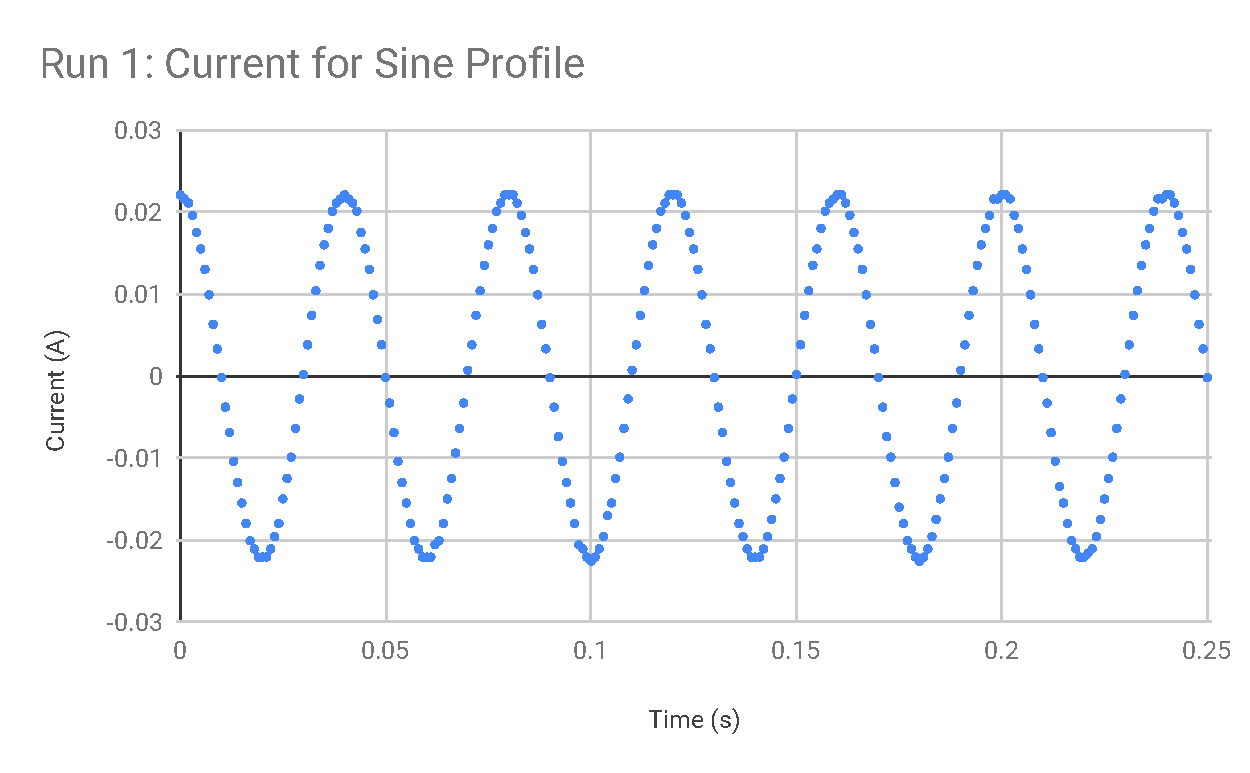
\includegraphics[scale=0.74]{image/04-faraday/run-1-I.pdf}
	\caption{Run 1: Current}
	\label{figure.04.run.1.I}
\end{figure}
%
\begin{figure}[ht]
	\centering
	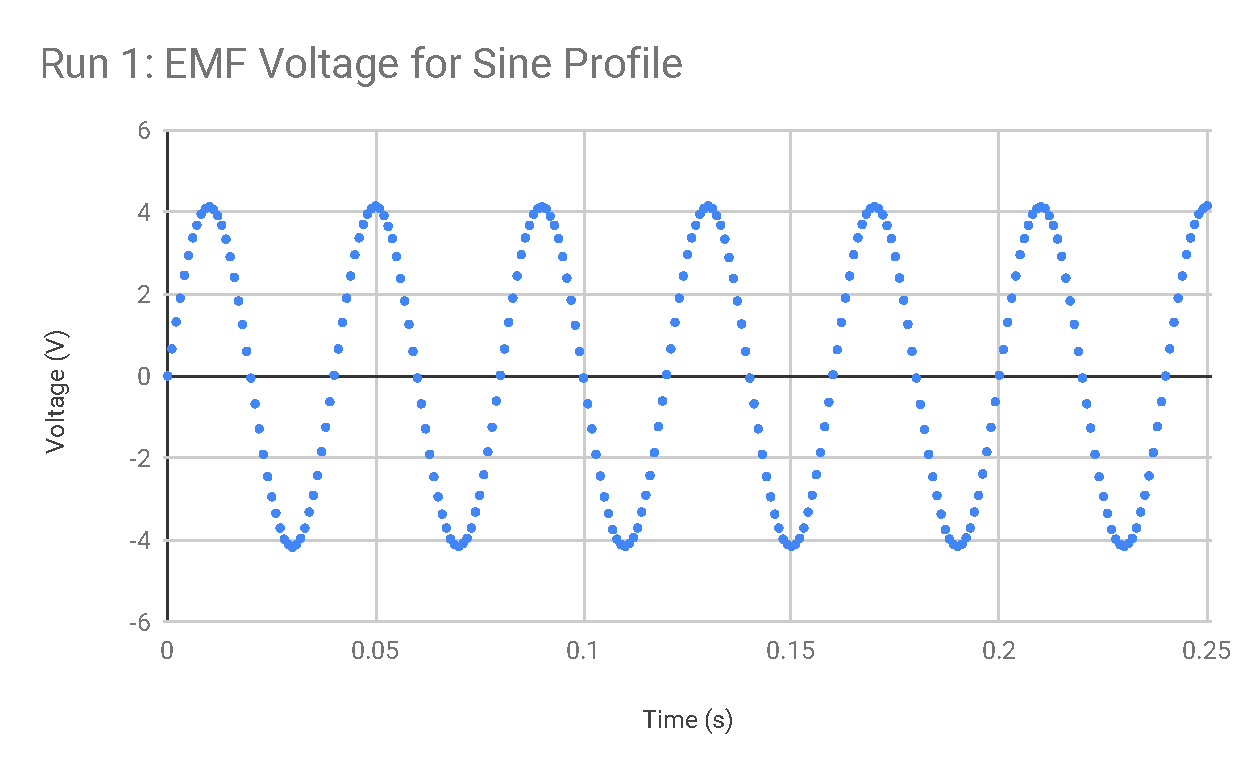
\includegraphics[scale=0.74]{image/04-faraday/run-1-V.pdf}
	\caption{Run 1: EMF Voltage}
	\label{figure.04.run.1.V}
\end{figure}
%
\begin{figure}[ht]
	\centering
	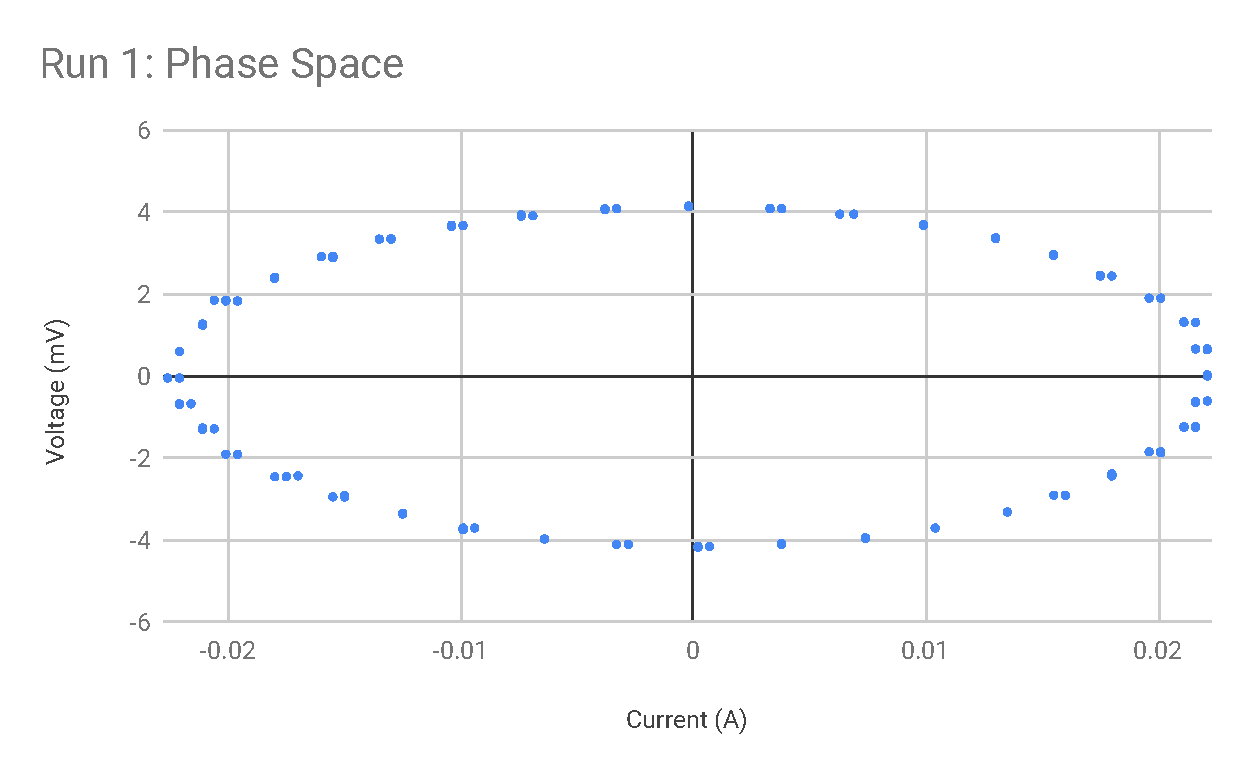
\includegraphics[scale=0.74]{image/04-faraday/run-1-phase-space.pdf}
	\caption{Run 1: Phase Space}
	\label{figure.04.run.1.phase.space}
\end{figure}
%
\begin{figure}[ht]
	\centering
	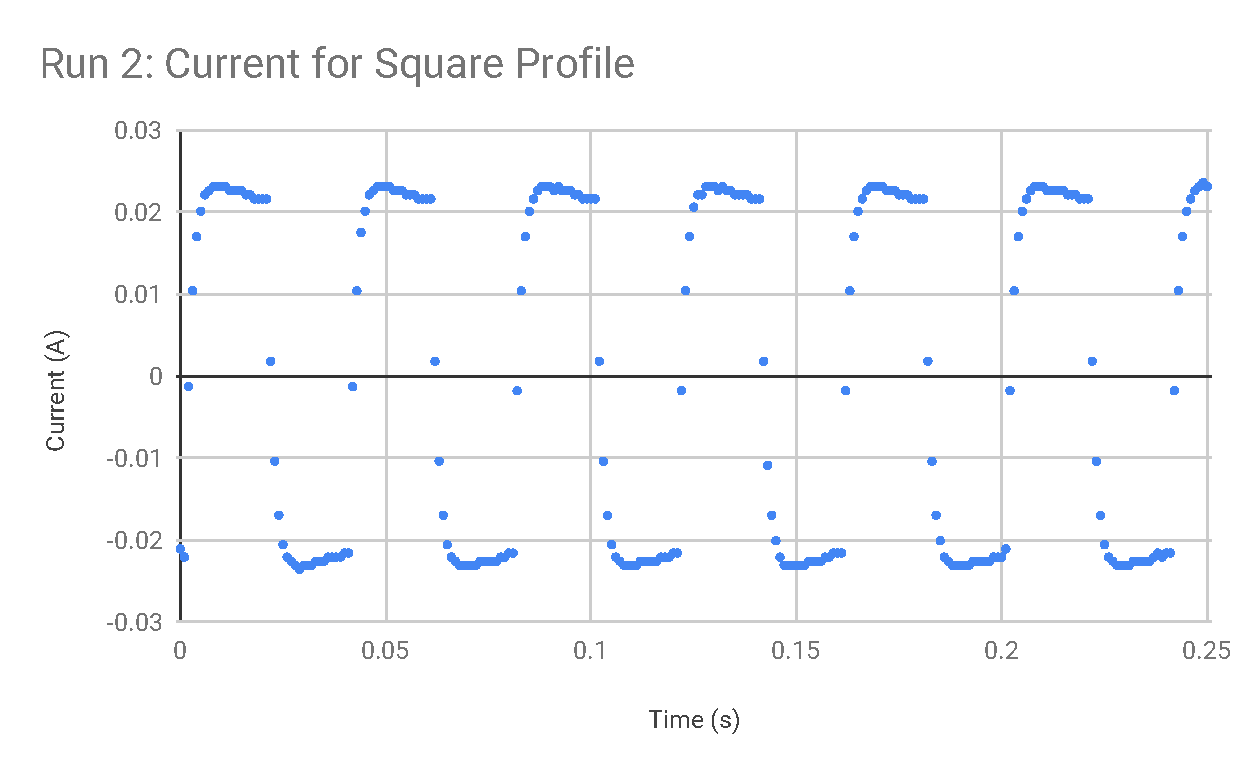
\includegraphics[scale=0.74]{image/04-faraday/run-2-I.pdf}
	\caption{Run 2: Current}
	\label{figure.04.run.2.I}
\end{figure}
%
\begin{figure}[ht]
	\centering
	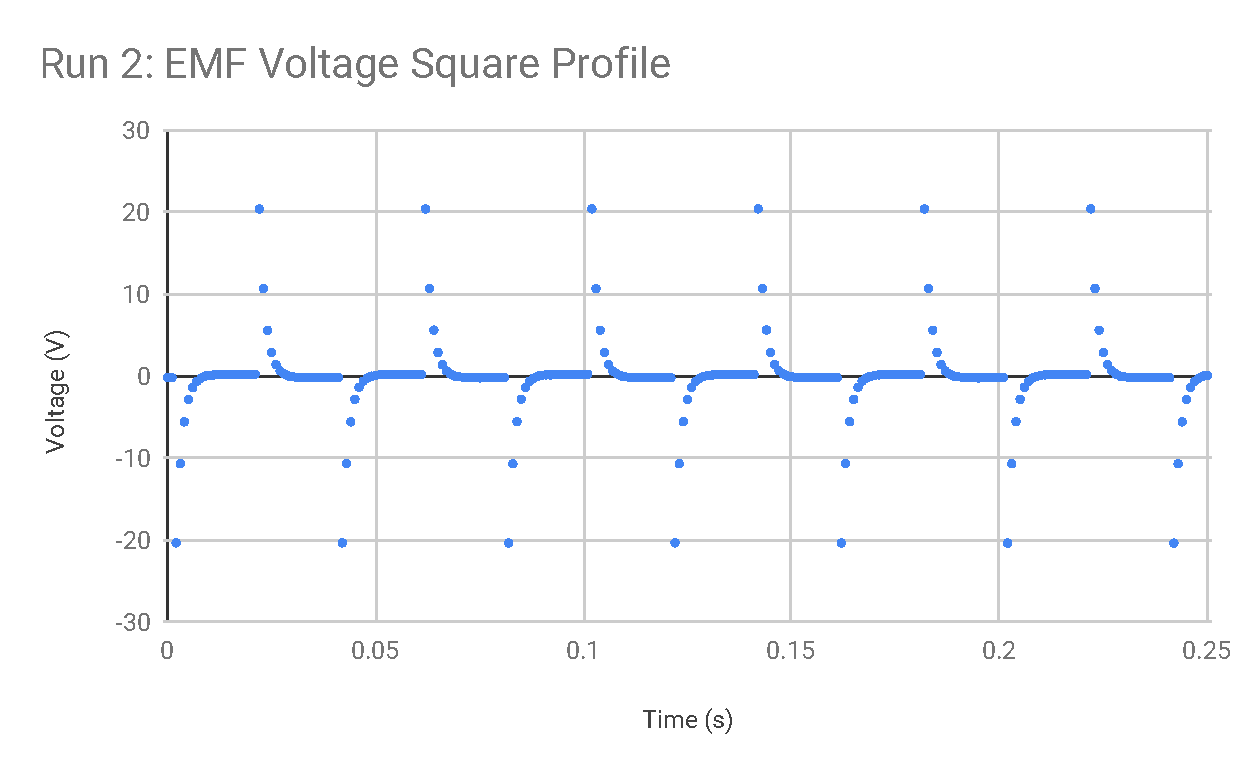
\includegraphics[scale=0.74]{image/04-faraday/run-2-V.pdf}
	\caption{Run 2: EMF Voltage}
	\label{figure.04.run.2.V}
\end{figure}
%
\begin{figure}[ht]
	\centering
	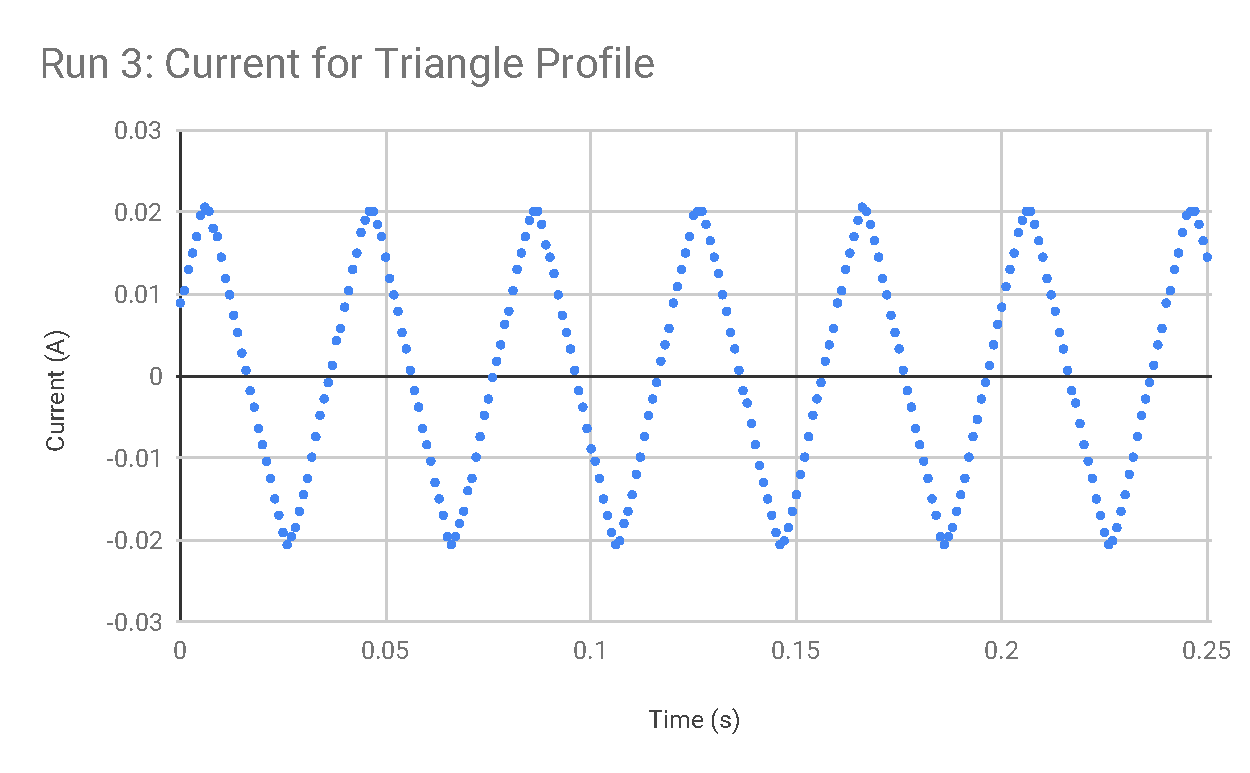
\includegraphics[scale=0.74]{image/04-faraday/run-3-I.pdf}
	\caption{Run 3: Current}
	\label{figure.04.run.3.I}
\end{figure}
%
\begin{figure}[ht]
	\centering
	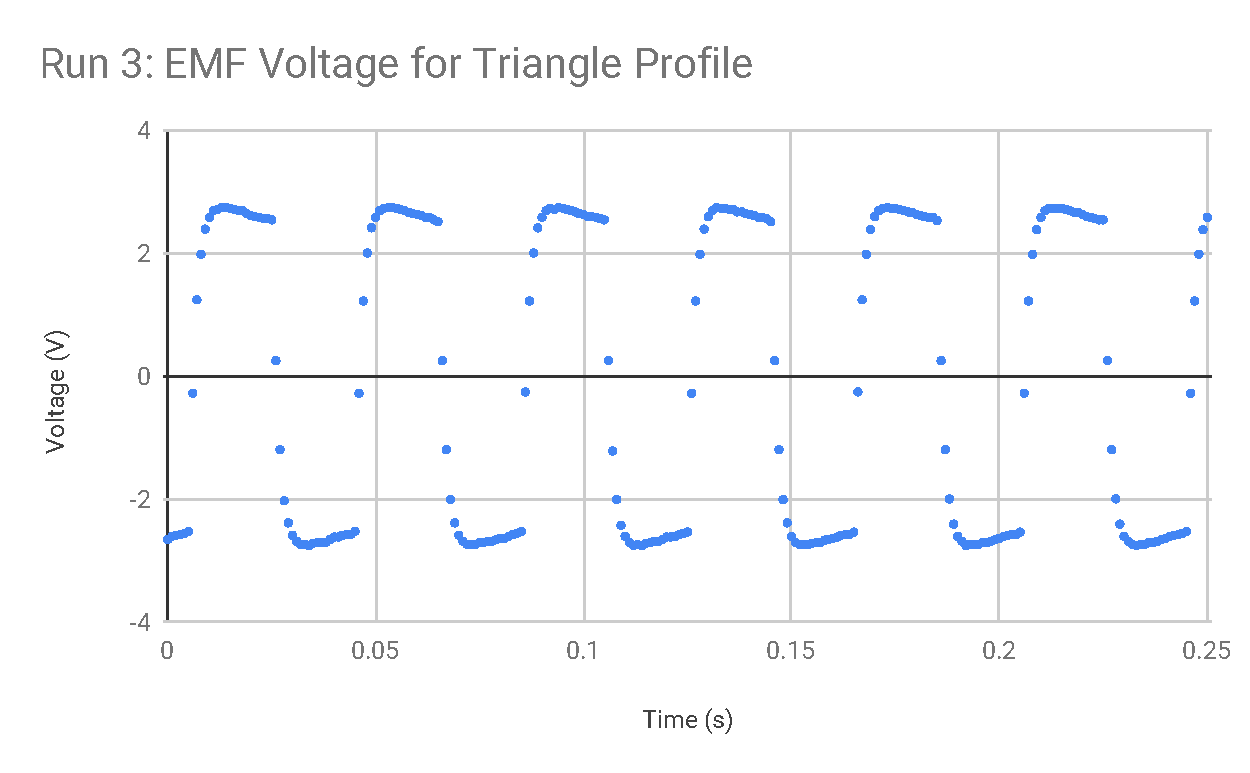
\includegraphics[scale=0.74]{image/04-faraday/run-3-V.pdf}
	\caption{Run 3: EMF Voltage}
	\label{figure.04.run.3.V}
\end{figure}
%
\begin{figure}[ht]
	\centering
	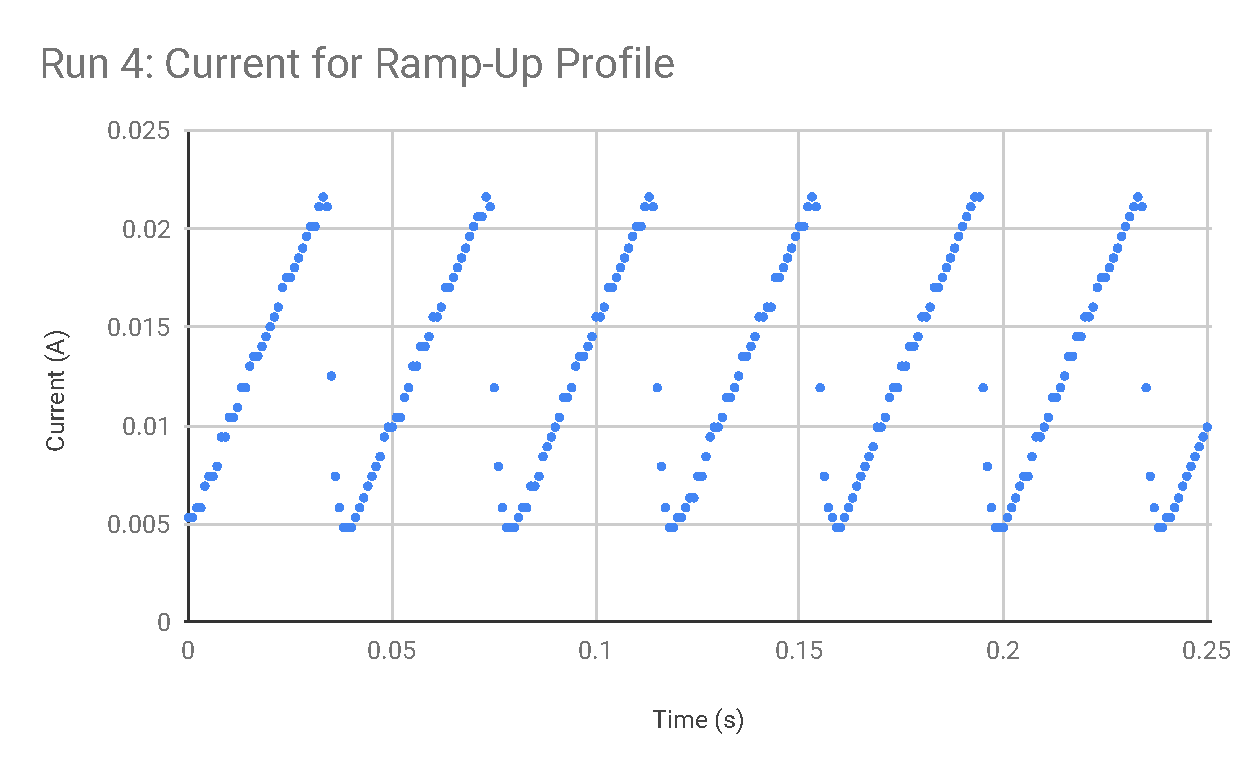
\includegraphics[scale=0.74]{image/04-faraday/run-4-I.pdf}
	\caption{Run 4: Current}
	\label{figure.04.run.4.I}
\end{figure}
%
\begin{figure}[ht]
	\centering
	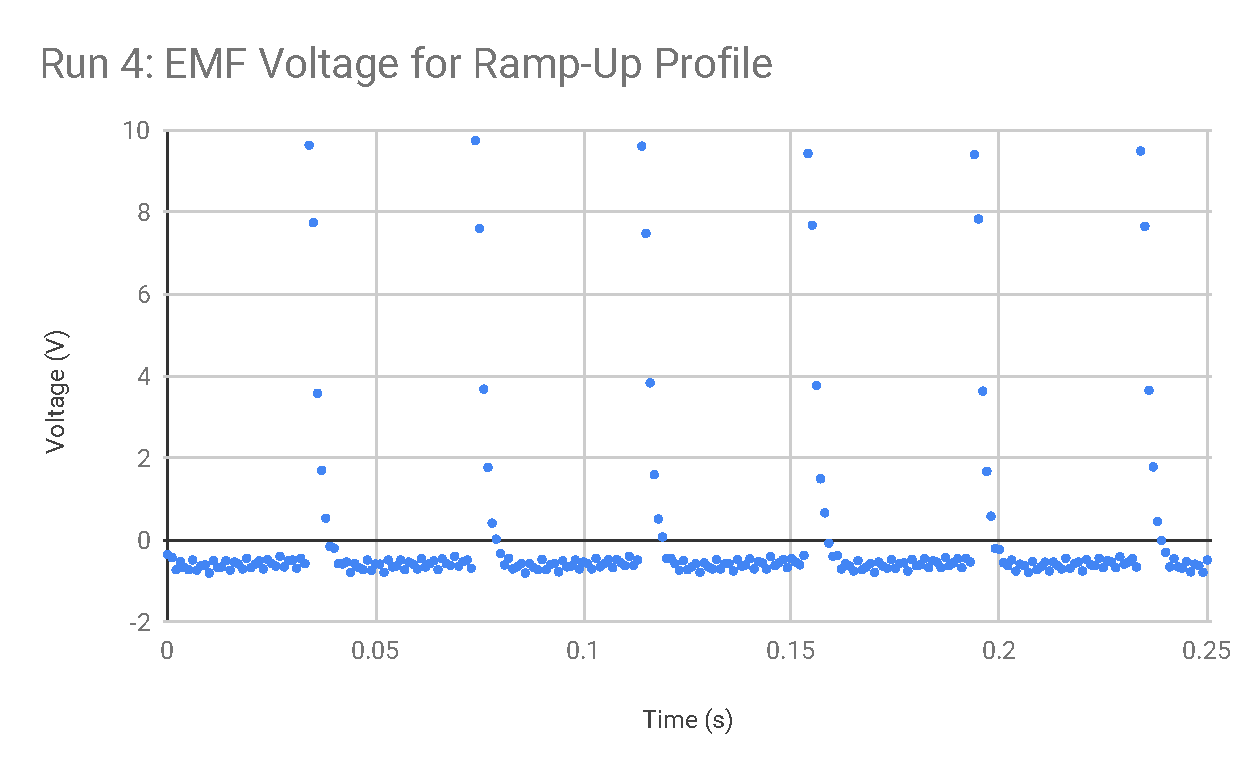
\includegraphics[scale=0.74]{image/04-faraday/run-4-V.pdf}
	\caption{Run 4: EMF Voltage}
	\label{figure.04.run.4.V}
\end{figure}
%
\begin{figure}[ht]
	\centering
	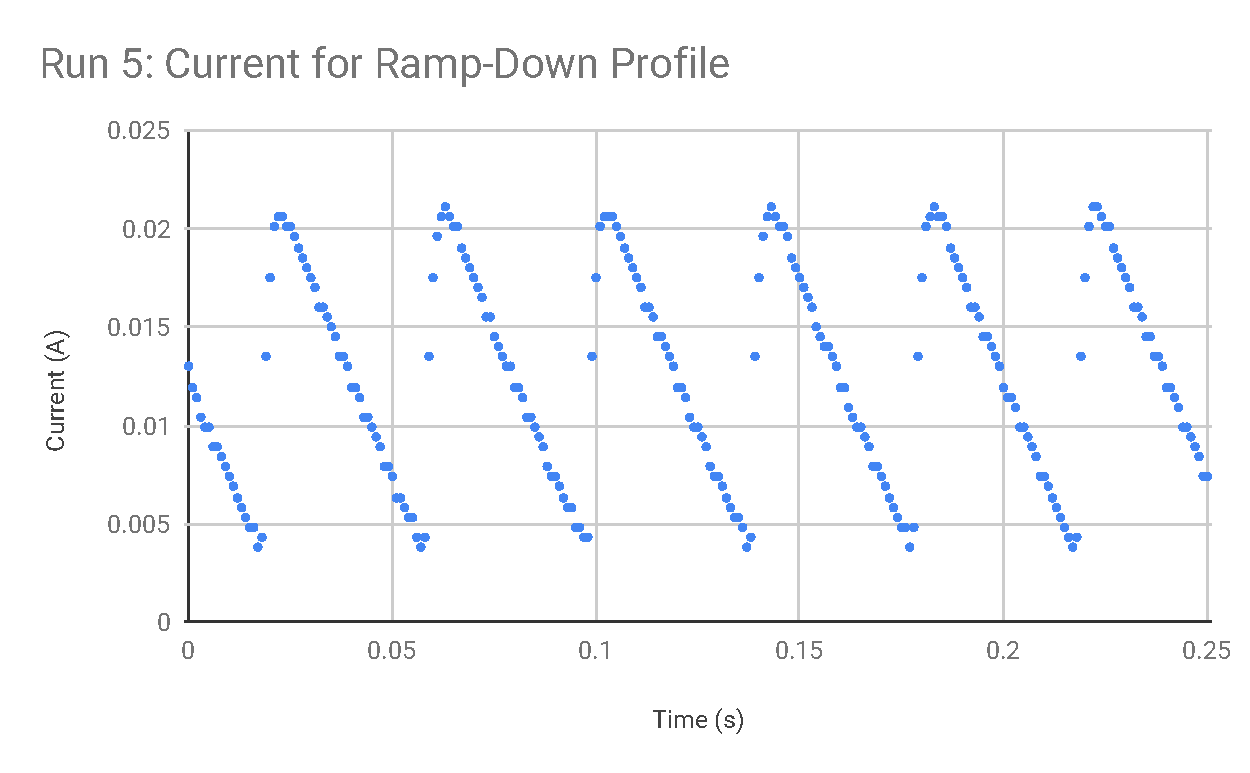
\includegraphics[scale=0.74]{image/04-faraday/run-5-I.pdf}
	\caption{Run 5: Current}
	\label{figure.04.run.5.I}
\end{figure}
%
\begin{figure}[ht]
	\centering
	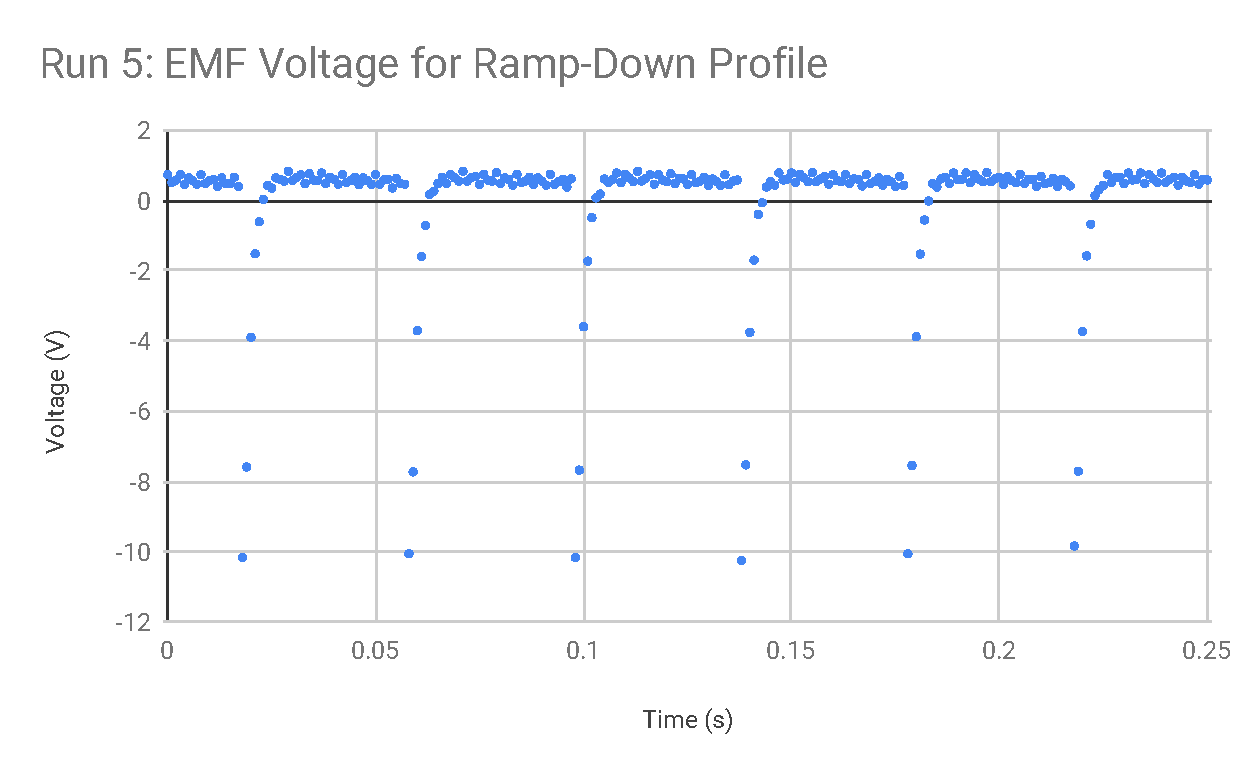
\includegraphics[scale=0.74]{image/04-faraday/run-5-V.pdf}
	\caption{Run 5: EMF Voltage}
	\label{figure.04.run.5.V}
\end{figure}
%
\begin{figure}[ht]
	\centering
	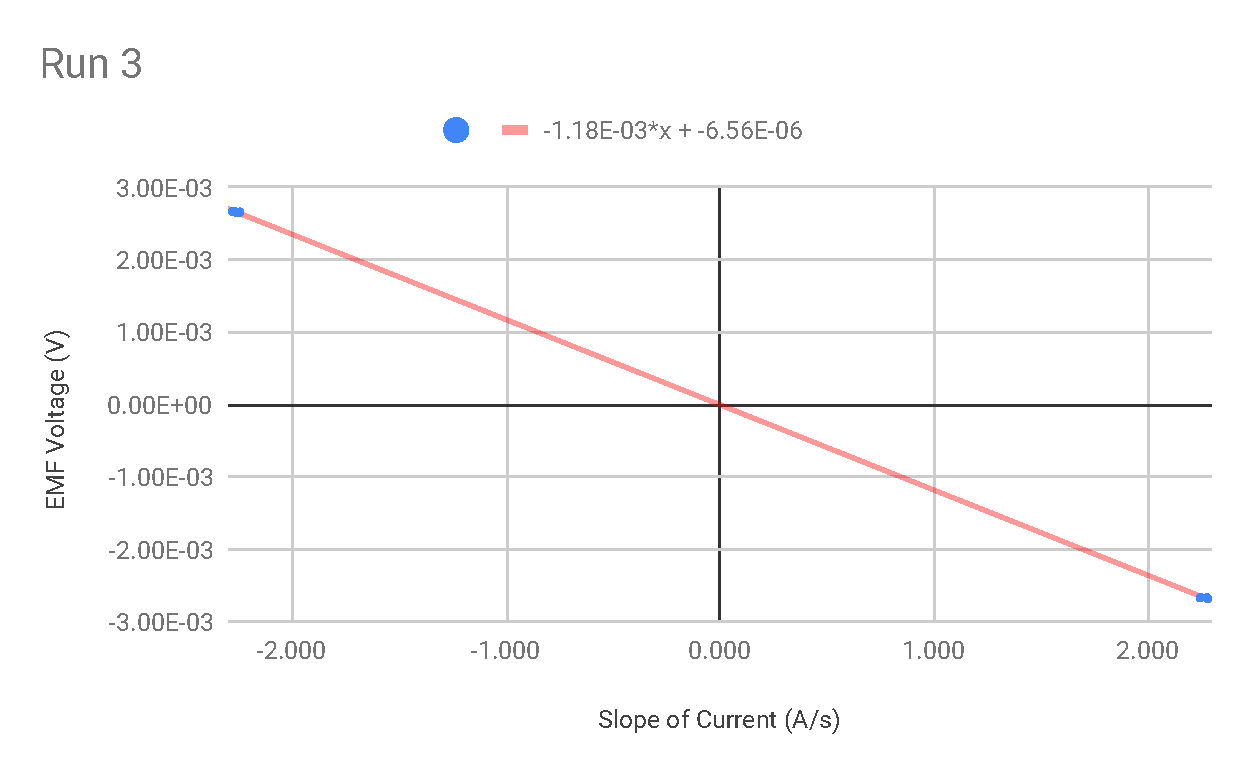
\includegraphics[scale=0.74]{image/04-faraday/run-3.pdf}
	\caption{Run 3}
	\label{figure.04.run.3}
\end{figure}
% % Copyright 2018-2020 Melvin Eloy Irizarry-Gelpí
\setcounter{chapter}{4}
\chapter{DC Circuits}
%%%%%%%%%%%%%%%%%%%%%%%%%%%%%%%%%%%%%%%%%%%%%%%%%%%%%%%%%%%%%%%%%%%%%%%%%%%%%%%%
In this experiment you will learn about circuits with DC sources, capacitors, and inductors.
%%%%%%%%%%%%%%%%%%%%%%%%%%%%%%%%%%%%%%%%%%%%%%%%%%%%%%%%%%%%%%%%%%%%%%%%%%%%%%%%
\section{Preliminary}
%%%%%%%%%%%%%%%%%%%%%%%%%%%%%%%%%%%%%%%%%%%%%%%%%%%%%%%%%%%%%%%%%%%%%%%%%%%%%%%%
In a previous experiment you constructed circuits with resistors and a battery. The resistors were connected either in series or in parallel. The battery served as a source producing a steady current. Such a source is called a \textbf{DC source}. Here DC stands for direct current, meaning that the current is always in the same direction along a circuit.

A circuit consisting exclusively of resistors and a DC source is not very interesting. Quantities like current and voltage in this circuit have fixed values over time. That is, when you flip a switch to complete the circuit, the current along the circuit jumps instantly to a non-zero value, and then does not change much. Similarly for the voltage across each resistor.

Besides resistors, you can have other components in a circuit with more complex physical properties like capacitance and inductance.
%%%%%%%%%%%%%%%%%%%%%%%%%%%%%%%%%%%%%%%%%%%%%%%%%%%%%%%%%%%%%%%%%%%%%%%%%%%%%%%%
\subsection{Resistance and Resistors}
%%%%%%%%%%%%%%%%%%%%%%%%%%%%%%%%%%%%%%%%%%%%%%%%%%%%%%%%%%%%%%%%%%%%%%%%%%%%%%%%
By now, electrical \textbf{resistance} should be familiar. The \textbf{SI unit} for electrical resistance is the \textbf{ohm}:
\begin{equation}
	1 \text{ ohm} = 1\;\Omega = 1 \text{ V/A}
\end{equation}
Here, V is volt (voltage) and A is ampere (current). A component in a circuit with a fixed amount of resistance is called a \textbf{resistor}. The mathematical symbol for resistance is $R$.
%%%%%%%%%%%%%%%%%%%%%%%%%%%%%%%%%%%%%%%%%%%%%%%%%%%%%%%%%%%%%%%%%%%%%%%%%%%%%%%%
\subsection{Capacitance and Capacitors}
%%%%%%%%%%%%%%%%%%%%%%%%%%%%%%%%%%%%%%%%%%%%%%%%%%%%%%%%%%%%%%%%%%%%%%%%%%%%%%%%
Another important property is \textbf{capacitance}. The \textbf{SI unit} for capacitance is the \textbf{farad}:
\begin{equation}
	1 \text{ farad} = 1 \text{ F} = 1 \text{ C/V}
\end{equation}
Here, C is coulomb (electric charge) and V is volt (voltage). In some ways, capacitance measures the amount of electric charge needed to sustain an electric potential difference (i.e. a voltage). The mathematical symbol for capacitance is $C$.

A component in a circuit with a fixed amount of capacitance is called a \textbf{capacitor}. You can think of a capacitor as two parallel plates of conducting material where equal-but-opposite amounts of electric charge can accumulate.
%%%%%%%%%%%%%%%%%%%%%%%%%%%%%%%%%%%%%%%%%%%%%%%%%%%%%%%%%%%%%%%%%%%%%%%%%%%%%%%%
\subsection{Inductance and Inductors}
%%%%%%%%%%%%%%%%%%%%%%%%%%%%%%%%%%%%%%%%%%%%%%%%%%%%%%%%%%%%%%%%%%%%%%%%%%%%%%%%
The last property is \textbf{inductance}, which is like a magnetic cousin of capacitance. The \textbf{SI unit} for inductance is the \textbf{henry}:
\begin{equation}
	1 \text{ henry} = 1 \text{ H} = 1 \text{ T}\cdot\text{m}^{2}\text{/A}
\end{equation}
Here, T is tesla (magnetic field), m$^{2}$ is square meter (area), and A is ampere (current). Recall that the tesla unit is equivalent to
\begin{equation}
    1 \text{ T} = 1 \text{ V} \cdot \text{s/m}^{2}
\end{equation}
Thus, the henry unit is equivalent to:
\begin{equation}
    1 \text{ H} = 1 \text{ V}\cdot\text{s/A}
\end{equation}
In some ways, inductance measures the amount of voltage that arises per unit rate of change of electric current with time. The mathematical symbol for inductance is $L$.

A component in a circuit with a fixed amount of inductance is called an \textbf{inductor}. You can think of an inductor as a solenoid coil with a given amount of loops, with each loop enclosing some amount of area.
%%%%%%%%%%%%%%%%%%%%%%%%%%%%%%%%%%%%%%%%%%%%%%%%%%%%%%%%%%%%%%%%%%%%%%%%%%%%%%%%
\subsubsection{Non-Ideal Inductors}
%%%%%%%%%%%%%%%%%%%%%%%%%%%%%%%%%%%%%%%%%%%%%%%%%%%%%%%%%%%%%%%%%%%%%%%%%%%%%%%%
An \textbf{ideal inductor} is a component in a circuit with \textbf{zero} electrical resistance and a desired amount of inductance. In practice, ideal inductors are usually not available and you usually use non-ideal inductors are used.

A \textbf{non-ideal inductor} is a component in a circuit with \textbf{non-zero} electrical resistance and non-zero amount of inductance. You can think of a non-ideal inductor as a resistor and an ideal inductor connected in series.
%%%%%%%%%%%%%%%%%%%%%%%%%%%%%%%%%%%%%%%%%%%%%%%%%%%%%%%%%%%%%%%%%%%%%%%%%%%%%%%%
\subsection{Exponential Decay Function}
%%%%%%%%%%%%%%%%%%%%%%%%%%%%%%%%%%%%%%%%%%%%%%%%%%%%%%%%%%%%%%%%%%%%%%%%%%%%%%%%
In a circuit with resistors and capacitors, or in a circuit with resistors and inductors, quantities like current and voltage do not always take steady values. That is because both capacitors and inductors can be thought of as storage containers for electric charge (or changing magnetic flux). These containers do not fill up instantly. Indeed, it can take a few seconds to fill-up a capacitor. The result is a behavior over time similar to an exponential decay curve.

Before discussing the behavior of quantities like current and voltage in circuits with capacitors and inductors in more detail, it will be good to review the \textbf{exponential decay} function:
\begin{equation}
    \exp(-t) = e^{-t}
\end{equation}
Here, $e$ is the \textbf{natural base}:
\begin{equation}
    e = 2.71828...
\end{equation}
When $t = 0$, the exponential decay function gives 1:
\begin{equation}
    \exp(0) = 1
\end{equation}
For large values of $t$, the exponential decay function approaches 0:
\begin{equation}
    \exp(-\infty) = 0
\end{equation}
In between $t = 0$ and $t \rightarrow \infty$ you have smaller and smaller values approaching zero.

The exponential decay function is an example of a function that is always positive, and always \textbf{decreasing} towards zero:
\begin{align}
    f(t) = \exp(-t) && 0 < f(t) \leq 1 && 0 \leq t < \infty
\end{align}
Multiplying the exponential decay function by a negative sign produces a function that is always negative, and always \textbf{increasing} towards zero:
\begin{align}
    g(t) = -\exp(-t) && -1 \leq g(t) < 0 && 0 \leq t < \infty
\end{align}
Another important combination is shifting vertically by 1, which gives a function that is always positive, and always \textbf{increasing} towards one:
\begin{align}
    h(t) = 1 - \exp(-t) && 0 \leq h(t) < 1 && 0 \leq t < \infty
\end{align}
Figures \ref{figure.05.f}, \ref{figure.05.g}, and \ref{figure.05.h} provide charts for these three functions.
%%%%%%%%%%%%%%%%%%%%%%%%%%%%%%%%%%%%%%%%%%%%%%%%%%%%%%%%%%%%%%%%%%%%%%%%%%%%%%%%
\subsection{Resistor and Capacitor in Series}
%%%%%%%%%%%%%%%%%%%%%%%%%%%%%%%%%%%%%%%%%%%%%%%%%%%%%%%%%%%%%%%%%%%%%%%%%%%%%%%%
A circuit with a resistor, a capacitor, and a DC source is called an \textbf{RC circuit}. In the simplest RC circuit, the resistor and capacitor are connected in series to the DC source via a particular switch.
%%%%%%%%%%%%%%%%%%%%%%%%%%%%%%%%%%%%%%%%%%%%%%%%%%%%%%%%%%%%%%%%%%%%%%%%%%%%%%%%
\subsubsection{Charging the Capacitor}
%%%%%%%%%%%%%%%%%%%%%%%%%%%%%%%%%%%%%%%%%%%%%%%%%%%%%%%%%%%%%%%%%%%%%%%%%%%%%%%%
When the switch is on, and the circuit is complete, the DC source pushes charges out into the circuit in the form of a current. This current causes positive electric charges to accumulate on one of the terminals of the capacitor, and negative electric charges on the other terminal of the capacitor. But the amount of electric charge $Q$ on the capacitor does not increase indefinitely: It settles on a maximum value $Q_{\infty}$. The particular manner in which the amount of \textbf{electric charge} on the capacitor increases with time is an example of an \textbf{exponential} increase:
\begin{equation}
    Q(t) = Q_{\infty} \left[ 1 - \exp\left(-\frac{t}{\tau_{C}}\right) \right]
    \label{eq.05.RC.q.charging}
\end{equation}
Here $Q_{\infty}$ is the amount of charge accumulated on the capacitor after an infinite amount of time, and $t$ correspond to the amount of time after the switch has been opened (the switch is opened at $t = 0$). The amount of \textbf{current} corresponds to the rate of change of the electric charge with respect to time:
\begin{equation}
    I(t) = I_{0} \exp\left(-\frac{t}{\tau_{C}}\right)
    \label{eq.05.RC.i.charging}
\end{equation}
For a capacitor with capacitance $C$, the amount of \textbf{voltage} $V_{C}$ across the \textbf{capacitor} is directly proportional to the amount of electric charge accumulated on the capacitor:
\begin{equation}
    V_{C}(t) = \frac{Q(t)}{C} = V_{\infty} \left[ 1 - \exp\left(-\frac{t}{\tau_{C}}\right) \right]
    \label{eq.05.RC.vC.charging}
\end{equation}
The constant of proportionality is the inverse of the capacitance.

The \textbf{voltage} $V_{R}$ across the \textbf{resistor} is directly proportional the the amount of current, via Ohm's law:
\begin{equation}
    V_{R}(t) = R I(t) = V_{\infty} \exp\left(-\frac{t}{\tau_{C}}\right)
    \label{eq.05.RC.vR.charging}
\end{equation}
Here, $V_{\infty}$ is related to $Q_{\infty}$ and/or $I_{0}$ via
\begin{eqnarray}
    V_{\infty} = \frac{Q_{\infty}}{C} = I_{0} R
\end{eqnarray}
The value of $V_{\infty}$ should correspond to the steady voltage across the DC source.

As you can see from (\ref{eq.05.RC.q.charging}), (\ref{eq.05.RC.i.charging}), and (\ref{eq.05.RC.vC.charging}), the amount of charge, current and voltage related to a capacitor all involve exponential functions. The constant $\tau_{C}$ is known as the \textbf{capacitive time constant}. It has units of time (seconds). The value of $\tau_{C}$ acts as a \textbf{time scale} for the change in values that occur. The same time scale appears in all three quantities.

In an RC circuit, the value of $\tau_{C}$ depends on how much resistance $R$ and capacitance $C$ you have:
\begin{equation}
    \tau_{C} = R C
    \label{eq.05.tauC}
\end{equation}
You can check that, in fact, by multiplying something with ohm units by something with farad units you get something with second units:
\begin{equation}
    1 \text{ ohm} \cdot 1 \text{ F} = \left(1 \text{ V}\cdot\text{ s/C}\right) \cdot \left(1 \text{ C/V}\right) = 1 \text{ s}
\end{equation}
Since the exponential function is a mathematical function that changes very fast, the current will take noise-level values after a time corresponding to about 5 capacitive time constants.
%%%%%%%%%%%%%%%%%%%%%%%%%%%%%%%%%%%%%%%%%%%%%%%%%%%%%%%%%%%%%%%%%%%%%%%%%%%%%%%%
\subsubsection{Discharging the Capacitor}
%%%%%%%%%%%%%%%%%%%%%%%%%%%%%%%%%%%%%%%%%%%%%%%%%%%%%%%%%%%%%%%%%%%%%%%%%%%%%%%%
After some time with the switch on, the amount of charge on the capacitor becomes almost constant (close to $Q_{\infty}$), the amount of voltage across the capacitor also becomes almost constant (close to $V_{\infty}$), and the current through the circuit becomes almost zero.

Upon opening the circuit by setting the switch off, the DC source stops supporting the charge accumulated on the capacitor, and that amount of charge begins to leave the capacitor. That is, the capacitor now is producing the current! The amount of charge on the capacitor follows a particular manner:
\begin{equation}
    Q(t) = Q_{0} \exp\left(-\frac{t}{\tau_{C}}\right)
    \label{eq.05.RC.q.discharging}
\end{equation}
Here $Q_{0}$ is the amount of charge at the moment that the switch is turned off. The electric current is given by
\begin{equation}
    I(t) = - I_{0} \exp\left(-\frac{t}{\tau_{C}}\right)
    \label{eq.05.RC.i.discharging}
\end{equation}
This behavior is very similar to the behavior of the current (\ref{eq.05.RC.i.charging}) while the capacitor is charging, except that the negative sign indicates the current is in the opposite direction, since the charge is leaving the capacitor. The voltage $V_{C}$ across the \textbf{capacitor} can, again, be found from the amount of electric charge:
\begin{equation}
    V_{C}(t) = \frac{Q(t)}{C} = V_{0} \exp\left(-\frac{t}{\tau_{C}}\right)
    \label{eq.05.RC.vC.discharging}
\end{equation}
The capacitive time constant appears again, and also dictates the time scale for the decrease of the charge, current and voltage across the capacitor during the discharging event. The voltage $V_{R}$ across the \textbf{resistor} can, again, be found from the amount of electric current:
\begin{equation}
    V_{R}(t) = R I(t) = - V_{0} \exp\left(-\frac{t}{\tau_{C}}\right)
\end{equation}
Just as before, there is a relation between $Q_{0}$, $I_{0}$, and $V_{0}$:
\begin{equation}
    V_{0} = \frac{Q_{0}}{C} = I_{0} R
\end{equation}
The value of $V_{0}$ should correspond to the voltage across the capacitor just before the switch is opened.
%%%%%%%%%%%%%%%%%%%%%%%%%%%%%%%%%%%%%%%%%%%%%%%%%%%%%%%%%%%%%%%%%%%%%%%%%%%%%%%%
\subsection{Resistor and Inductor in Series}
%%%%%%%%%%%%%%%%%%%%%%%%%%%%%%%%%%%%%%%%%%%%%%%%%%%%%%%%%%%%%%%%%%%%%%%%%%%%%%%%
A circuit with a resistor, an inductor, and a DC source is called an \textbf{RL circuit}. In the simplest RL circuit, the resistor and inductor are connected in series to the DC source via a particular switch.

An \textbf{ideal inductor} is an inductor that has \textbf{zero electrical resistance}. In practice, the inductors that you will use in these experiments have an amount of resistance that cannot be ignored and has to be taken into account. One way to do this is to think of a \textbf{non-ideal inductor} as consisting of a resistor and an ideal inductor connected in series:
\begin{equation}
    \text{non-ideal inductor} = \text{resistor} + \text{ideal inductor in series}
\end{equation}
Thus, an RL circuit with one resistor with resistance $R$ and one non-ideal inductor with resistance $r$ and inductance $L$ in series is equivalent to an RL circuit with \textbf{two} resistors and one ideal inductor in series. Let $V_{0}$ correspond to the steady voltage produced by the DC source in the RL circuit. Then, since the circuit is in series, the amount of steady voltage from the DC source must be equivalent to the sum of voltages across the two resistors and the ideal inductor:
\begin{equation}
    V_{0} = V_{R}(t) + V_{r}(t) + V_{L}(t)
\end{equation}
Here, $V_{R}$ is the voltage across the main resistor, $V_{r}$ is the voltage across the resistor within the non-ideal inductor, and $V_{L}$ is the voltage across the ideal inductor. The problem is that you can directly measure $V_{R}$, but not $V_{L}$. Instead, measuring the voltage across the inductor gives the non-ideal total $V_{N} = V_{r} + V_{L}$. The other problem is that $V_{L}$ is what you really want, so $V_{r}$ has to be subtracted from $V_{N}$:
\begin{equation}
    V_{L}(t) = V_{N}(t) - V_{r}(t)
\end{equation}
Although an inductor does not accumulate electric charge like a capacitor, the behavior of electric current and voltage across an inductor in an RL circuit also involves \textbf{exponential} functions. Whereas in an RC circuit the current becomes zero for large time values after closing the switch, in an RL circuit the current rises to a steady value:
\begin{equation}
    I(t) = I_{\infty} \left[ 1 - \exp\left(- \frac{t}{\tau_{L}}\right) \right]
    \label{eq.05.RL.i.rise}
\end{equation}
The \textbf{voltage} $V_{R}$ across the main \textbf{resistor} is given by Ohm's law:
\begin{equation}
    V_{R}(t) = R I(t) = R I_{\infty} \left[ 1 - \exp\left(- \frac{t}{\tau_{L}}\right) \right]
    \label{eq.05.RL.vR}
\end{equation}
The \textbf{voltage} $V_{r}$ across the resistor within the non-ideal inductor is also given by Ohm's law:
\begin{equation}
    V_{r}(t) = r I(t) = r I_{\infty} \left[ 1 - \exp\left(- \frac{t}{\tau_{L}}\right) \right]
    \label{eq.05.RL.vr}
\end{equation}
The \textbf{voltage} $V_{L}$ across the \textbf{ideal inductor} is given by
\begin{equation}
    V_{L}(t) = V_{0} - V_{R}(t) - V_{r}(t) = V_{0} \exp\left(- \frac{t}{\tau_{L}}\right)
    \label{eq.05.RL.vL}
\end{equation}
Here $I_{\infty}$ and $V_{0}$ are related via
\begin{equation}
    V_{0} = I_{\infty} \left(R + r\right)
\end{equation}
Instead of $\tau_{C}$, you now have $\tau_{L}$ which corresponds to the \textbf{inductive time constant}. Just like $\tau_{C}$, the value of $\tau_{L}$ depends on the total amount of resistance and also on the inductance you have in the circuit:
\begin{equation}
    \tau_{L} = \frac{L}{R + r}
    \label{eq.05.tauL}
\end{equation}
You can check that, in fact, by dividing something with henry units by something with ohm units you get something with second units.
%%%%%%%%%%%%%%%%%%%%%%%%%%%%%%%%%%%%%%%%%%%%%%%%%%%%%%%%%%%%%%%%%%%%%%%%%%%%%%%%
\section{Experiment}
%%%%%%%%%%%%%%%%%%%%%%%%%%%%%%%%%%%%%%%%%%%%%%%%%%%%%%%%%%%%%%%%%%%%%%%%%%%%%%%%
You did experiments with both RC and RL circuits.
%%%%%%%%%%%%%%%%%%%%%%%%%%%%%%%%%%%%%%%%%%%%%%%%%%%%%%%%%%%%%%%%%%%%%%%%%%%%%%%%
\subsection{RC Circuits}
%%%%%%%%%%%%%%%%%%%%%%%%%%%%%%%%%%%%%%%%%%%%%%%%%%%%%%%%%%%%%%%%%%%%%%%%%%%%%%%%
For RC circuits there are two kinds of experiments: the \textbf{charging} event and the \textbf{discharging} event. In each experiment you measured three quantities:
\begin{itemize}
    \item the \textbf{voltage} across the \textbf{resistor}, $V_{R}(t)$;
    \item the \textbf{current} flowing between the resistor and the capacitor, $I(t)$; and
    \item the \textbf{voltage} across the \textbf{capacitor}, $V_{C}(t)$.
\end{itemize}
For the \textbf{charging event}, the data collection was started with the switch off (i.e. incomplete circuit) and shortly after the switch was turned on. You should analyze the \textbf{current} and the \textbf{voltage across the resistor} for such events.

For the \textbf{discharging event}, the data collection was started with the switch on (i.e. complete circuit) and shortly after the switch was turned off. You should analyze the \textbf{voltage across the capacitor} for such events.

There are many resistors and capacitors available. Each time the resistance or the capacitance changes, the time constant $\tau_{C}$ will also change.
%%%%%%%%%%%%%%%%%%%%%%%%%%%%%%%%%%%%%%%%%%%%%%%%%%%%%%%%%%%%%%%%%%%%%%%%%%%%%%%%
\subsection{Non-Ideal Inductors}
%%%%%%%%%%%%%%%%%%%%%%%%%%%%%%%%%%%%%%%%%%%%%%%%%%%%%%%%%%%%%%%%%%%%%%%%%%%%%%%%
You need to take into account the electrical resistance of the inductor used because it is non-ideal. In order to obtain the resistance of the inductor, you use a circuit with the inductor and the DC source (an L DC circuit) and measure the current through the circuit and the voltage across the inductor.

The solenoid inductors that are available come with a metallic core that can be inserted inside the solenoid. It is good to check that the resistance of the non-ideal inductor is not affected by using the metallic core.

When two resistors are connected in series, the equivalent resistance is the sum of the individual resistances. In a similar way, you can check that connecting two non-ideal inductors in series yields an equivalent non-ideal inductor with a resistance corresponding to the sum of the resistances of each non-ideal inductor.
%%%%%%%%%%%%%%%%%%%%%%%%%%%%%%%%%%%%%%%%%%%%%%%%%%%%%%%%%%%%%%%%%%%%%%%%%%%%%%%%
\subsection{RL Circuits}
%%%%%%%%%%%%%%%%%%%%%%%%%%%%%%%%%%%%%%%%%%%%%%%%%%%%%%%%%%%%%%%%%%%%%%%%%%%%%%%%
For RL circuits, all the experiments involved closing the switch after the data collection was started. You measured
\begin{itemize}
    \item the \textbf{voltage} across the resistor, $V_{R}(t)$;
    \item the \textbf{current} flowing between the resistor and the non-ideal inductor, $I(t)$; and
    \item the \textbf{voltage} across the non-ideal inductor, $V_{N}(t)$.
\end{itemize}
Because the inductive time constants are so small, the data acquisition needs to be activated with the trigger feature.

The inductors come with a \textbf{metallic core}. Each experiment is done twice: Once without the core, and once with the core. The effect of the core is to change the inductance of the inductor.

There are many resistors, and many ways to connect inductors of the same type. Each time the resistance or the inductance changes, the time constant $\tau_{L}$ will also change.
%%%%%%%%%%%%%%%%%%%%%%%%%%%%%%%%%%%%%%%%%%%%%%%%%%%%%%%%%%%%%%%%%%%%%%%%%%%%%%%%
\section{Analysis}
%%%%%%%%%%%%%%%%%%%%%%%%%%%%%%%%%%%%%%%%%%%%%%%%%%%%%%%%%%%%%%%%%%%%%%%%%%%%%%%%
The common feature of $f(t)$, $g(t)$, and $h(t)$ above is that they all settle on steady values for infinite time after $t = 0$. In an experiment, you do not have an infinite amount of time, so a relevant question is: how long corresponds to infinite time? Since you are using imperfect sensors to measure current and voltage, after some time of decreasing values towards zero, there will be a point where measurements are not distinguishable from noise.

Consider the following function:
\begin{equation}
    A(t) = A_{0} \exp\left(- \frac{t}{\tau}\right)
\end{equation}
At $t = 0$, you have
\begin{equation}
    A(0) = A_{0}
\end{equation}
Thus, $A_{0}$ correspond to the amount of $A$ present at $t = 0$. The value of $A$ after one unit of $\tau$ is:
\begin{equation}
    A(\tau) = A_{0} \exp\left(-1\right) = 0.3679 \cdot A_{0}
\end{equation}
That is, about 37\% of the starting value. After two units of $\tau$ you have:
\begin{equation}
    A(2\tau) = A_{0} \exp\left(-2\right) = 0.1353 \cdot A_{0}
\end{equation}
That is, about 14\% of the starting value. After three units of $\tau$ you have:
\begin{equation}
    A(3\tau) = A_{0} \exp\left(-3\right) = 0.0498 \cdot A_{0}
\end{equation}
That is, about 5\% of the starting value. After four units of $\tau$ you have:
\begin{equation}
    A(4\tau) = A_{0} \exp\left(-4\right) = 0.0183 \cdot A_{0}
\end{equation}
That is, about 2\% of the starting value. After five units of $\tau$ you have:
\begin{equation}
    A(5\tau) = A_{0} \exp\left(-5\right) = 0.0067 \cdot A_{0}
\end{equation}
That is, about 0.67\% of the starting value. Five units of $\tau$ is a good rule of thumb. In principle, the quantity that is being measured will continue decreasing in value, but in practice those small values cannot be reliably measured. If you have an estimate of the amount of $\tau$, then from the time the decay begins you should keep data until after $5 \tau$ of time has passed.
%%%%%%%%%%%%%%%%%%%%%%%%%%%%%%%%%%%%%%%%%%%%%%%%%%%%%%%%%%%%%%%%%%%%%%%%%%%%%%%%
%%%%%%%%%%%%%%%%%%%%%%%%%%%%%%%%%%%%%%%%%%%%%%%%%%%%%%%%%%%%%%%%%%%%%%%%%%%%%%%%
\subsection{RC Circuits: Charging Events}
%%%%%%%%%%%%%%%%%%%%%%%%%%%%%%%%%%%%%%%%%%%%%%%%%%%%%%%%%%%%%%%%%%%%%%%%%%%%%%%%
In a charging even both the voltage across the resistor and the current decay exponentially. Here are some steps to follow:
%%%%%%%%%%%%%%%%%%%%%%%%%%%%%%%%%%%%%%%%%%%%%%%%%%%%%%%%%%%%%%%%%%%%%%%%%%%%%%%%
\subsubsection{Visualize $V_{R}$ and $I$}
%%%%%%%%%%%%%%%%%%%%%%%%%%%%%%%%%%%%%%%%%%%%%%%%%%%%%%%%%%%%%%%%%%%%%%%%%%%%%%%%
Make two scatter charts:
\begin{itemize}
    \item Voltage across the resistor in the vertical axis, and time in the horizontal axis.
    \item Current in the vertical axis, and time in the horizontal axis.
\end{itemize}
You might want to add exponential fits, although at this stage they would most likely not be appropriate. See Figure \ref{figure.05.run.1.vR.full} for an example.
%%%%%%%%%%%%%%%%%%%%%%%%%%%%%%%%%%%%%%%%%%%%%%%%%%%%%%%%%%%%%%%%%%%%%%%%%%%%%%%%
\subsubsection{Truncate the part before closing circuit}
%%%%%%%%%%%%%%%%%%%%%%%%%%%%%%%%%%%%%%%%%%%%%%%%%%%%%%%%%%%%%%%%%%%%%%%%%%%%%%%%
Before the exponential fit can be made meaningful, you need to truncate the part of the data before the switch is closed. Looking at the columns, it should be obvious when the values for $V_{R}$ and $I$ suddenly take large values. See Figure \ref{figure.05.run.1.vR.truncated} for an example after truncation.
%%%%%%%%%%%%%%%%%%%%%%%%%%%%%%%%%%%%%%%%%%%%%%%%%%%%%%%%%%%%%%%%%%%%%%%%%%%%%%%%
\subsubsection{Truncate the long tail}
%%%%%%%%%%%%%%%%%%%%%%%%%%%%%%%%%%%%%%%%%%%%%%%%%%%%%%%%%%%%%%%%%%%%%%%%%%%%%%%%
It is very likely that after removing the part of the data before closing the circuit, the exponential fit might still not be appropriate. If the decay is relatively quick, and the voltage or current has a long segment where it is just zero, that long tail section will skew the fit process and render incorrect results. For this reason, it is good to only keep a time segment that is about $5\tau_{C}$ long. For example, after truncation in Figure \ref{figure.05.run.1.vR.truncated}, the decay begins around $t = 1.85$ seconds. For this particular run, the expected value of the time constant is $\tau_{C} = 0.250$ seconds. Thus,
\begin{equation}
    1.85 \text{ s} + 5 \tau_{C} = 3.10 \text{ s}
\end{equation}
All the data after $t = 3.10$ seconds should be truncated also. For good measure, I am keeping everything up to $t = 3.20$ seconds. See Figure \ref{figure.05.run.1.vR.no.tail} for an example.
%%%%%%%%%%%%%%%%%%%%%%%%%%%%%%%%%%%%%%%%%%%%%%%%%%%%%%%%%%%%%%%%%%%%%%%%%%%%%%%%
\subsubsection{Extract the experimental value of $\tau_{C}$}
%%%%%%%%%%%%%%%%%%%%%%%%%%%%%%%%%%%%%%%%%%%%%%%%%%%%%%%%%%%%%%%%%%%%%%%%%%%%%%%%
After truncating the initial and long tail parts, the exponential fit should be appropriate for the data. The exponential fit is given in the form
\begin{equation}
    a \exp(-bx)
\end{equation}
The value of $b$ corresponds to the inverse of the time constant:
\begin{equation}
    b = \frac{1}{\tau_{C}}
\end{equation}
Thus, the observed value of the time constant follows from the inverse of $b$:
\begin{equation}
    \text{Observed } \tau_{C} = \frac{1}{b}
\end{equation}
You should get a value from the $V_{R}$ chart, and another value from the $I$ chart. Both values should be consistent with each other.
%%%%%%%%%%%%%%%%%%%%%%%%%%%%%%%%%%%%%%%%%%%%%%%%%%%%%%%%%%%%%%%%%%%%%%%%%%%%%%%%
\subsection{RC Circuits: Discharging Events}
%%%%%%%%%%%%%%%%%%%%%%%%%%%%%%%%%%%%%%%%%%%%%%%%%%%%%%%%%%%%%%%%%%%%%%%%%%%%%%%%
In the discharging event, only the voltage across the capacitor follows an exponential decay. The steps are similar:
\begin{enumerate}
    \item Visualize the data with a scatter chart with the voltage across the capacitor in the vertical axis, and time in the horizontal axis.
    \item Truncate the part before opening the circuit.
    \item Truncate the long tail and keep close to $5\tau_{C}$ after the time the decay begins.
    \item Extract the experimental value of $\tau_{C}$ from the fit equation.
\end{enumerate}
The value of $\tau_{C}$ for the discharging even should be consistent with the values for the charging event.
%%%%%%%%%%%%%%%%%%%%%%%%%%%%%%%%%%%%%%%%%%%%%%%%%%%%%%%%%%%%%%%%%%%%%%%%%%%%%%%%
\subsection{RL Circuits: Resistance of Inductors}
%%%%%%%%%%%%%%%%%%%%%%%%%%%%%%%%%%%%%%%%%%%%%%%%%%%%%%%%%%%%%%%%%%%%%%%%%%%%%%%%
Before dealing with the inductive time constant experiments, you have to determine how much electrical resistance does the non-ideal inductors that are available have. Just like for resistors, in order to obtain resistance you measure current and voltage data over time. Using
\begin{equation}
    r = \frac{V_{r}(t)}{I(t)}
\end{equation}
should provide the observed value of the resistance of the non-ideal inductor over time. This value should be steady and almost constant, so take a time average to get the best estimate.

For two non-ideal inductors in series, you should find that the resistance is close to double the resistance for a single non-ideal inductor in series. This is consistent with the rule
\begin{equation}
    R_{\text{eq}} = R_{1} + R_{2}
\end{equation}
For a single non-ideal inductor, you should find a resistance close to 4.2 ohms. For two non-ideal inductors, you should find a resistance close to 8.5 ohms.
%%%%%%%%%%%%%%%%%%%%%%%%%%%%%%%%%%%%%%%%%%%%%%%%%%%%%%%%%%%%%%%%%%%%%%%%%%%%%%%%
\section{My Data}
%%%%%%%%%%%%%%%%%%%%%%%%%%%%%%%%%%%%%%%%%%%%%%%%%%%%%%%%%%%%%%%%%%%%%%%%%%%%%%%%
...
%%%%%%%%%%%%%%%%%%%%%%%%%%%%%%%%%%%%%%%%%%%%%%%%%%%%%%%%%%%%%%%%%%%%%%%%%%%%%%%%
\section{Your Data}
%%%%%%%%%%%%%%%%%%%%%%%%%%%%%%%%%%%%%%%%%%%%%%%%%%%%%%%%%%%%%%%%%%%%%%%%%%%%%%%%
...
%%%%%%%%%%%%%%%%%%%%%%%%%%%%%%%%%%%%%%%%%%%%%%%%%%%%%%%%%%%%%%%%%%%%%%%%%%%%%%%%
\newpage
\section{Your Report}
%%%%%%%%%%%%%%%%%%%%%%%%%%%%%%%%%%%%%%%%%%%%%%%%%%%%%%%%%%%%%%%%%%%%%%%%%%%%%%%%
...
%%%%%%%%%%%%%%%%%%%%%%%%%%%%%%%%%%%%%%%%%%%%%%%%%%%%%%%%%%%%%%%%%%%%%%%%%%%%%%%%
\newpage
\section{Tables}
%%%%%%%%%%%%%%%%%%%%%%%%%%%%%%%%%%%%%%%%%%%%%%%%%%%%%%%%%%%%%%%%%%%%%%%%%%%%%%%%
\begin{table}[ht!]
    \begin{center}
        \begin{tabular}{|l|r|r|r|r|r|}
            \hline
            Run & $R$ (ohm) & $C$ (F) & Expected $\tau_{C}$ (s) & Observed $\tau_{C}$ (s) & P.D. (\%) \\
            \hline
            1.1 & 10 & 0.025 & 0.2500 & 0.2950 & 17.9941 \\
            1.2 & 10 & 0.025 & 0.2500 & 0.3033 & 20.1201 \\
            3.1 & 51 & 0.025 & 1.2750 & 1.4327 & 12.3659 \\
            3.2 & 68 & 0.025 & 1.7000 & 1.8904 & 11.1976 \\
            5.1 & $2.2 \times 10^{4}$ & $10^{-5}$ & 0.2200 & 0.2674 & 21.5362 \\
            5.2 & $4.7 \times 10^{4}$ & $10^{-5}$ & 0.4700 & 0.5495 & 16.9044 \\
            \hline
        \end{tabular}
    \end{center}
    \caption{Results for $\tau_{C}$ from $V_{R}$ (charging)}
\end{table}
%%%%%%%%%%%%%%%%%%%%%%%%%%%%%%%%%%%%%%%%%%%%%%%%%%%%%%%%%%%%%%%%%%%%%%%%%%%%%%%%
\begin{table}[ht!]
    \begin{center}
        \begin{tabular}{|l|r|r|r|r|r|}
            \hline
            Run & $R$ (ohm) & $C$ (F) & Expected $\tau_{C}$ (s) & Observed $\tau_{C}$ (s) & P.D. (\%) \\
            \hline
            1.1 & 10 & 0.025 & 0.2500 & 0.2950 & 17.9941 \\
            1.2 & 10 & 0.025 & 0.2500 & 0.2994 & 19.7605 \\
            3.1 & 51 & 0.025 & 1.2750 & 1.4265 & 11.8850 \\
            3.2 & 68 & 0.025 & 1.7000 & 1.8939 & 11.4082 \\
            \hline
        \end{tabular}
    \end{center}
    \caption{Results for $\tau_{C}$ from $I$ (charging)}
\end{table}
%%%%%%%%%%%%%%%%%%%%%%%%%%%%%%%%%%%%%%%%%%%%%%%%%%%%%%%%%%%%%%%%%%%%%%%%%%%%%%%%
\begin{table}[ht!]
    \begin{center}
        \begin{tabular}{|l|r|r|r|r|r|}
            \hline
            Run & $R$ (ohm) & $C$ (F) & Expected $\tau_{C}$ (s) & Observed $\tau_{C}$ (s) & P.D. (\%) \\
            \hline
            2.1 & 10 & 0.025 & 0.2500 & 0.2618 & 4.7120 \\
            2.2 & 10 & 0.025 & 0.2500 & 0.2625 & 4.9869 \\
            4.1 & 51 & 0.025 & 1.2750 & 1.3680 & 7.2933 \\
            4.2 & 68 & 0.025 & 1.7000 & 1.8149 & 6.7578 \\
            6.1 & $2.2 \times 10^{4}$ & $10^{-5}$ & 0.2200 & 0.2674 & 16.5501 \\
            6.2 & $4.7 \times 10^{4}$ & $10^{-5}$ & 0.4700 & 0.5495 & 15.6337 \\
            \hline
        \end{tabular}
    \end{center}
    \caption{Results for $\tau_{C}$ from $V_{C}$ (discharging)}
\end{table}
%%%%%%%%%%%%%%%%%%%%%%%%%%%%%%%%%%%%%%%%%%%%%%%%%%%%%%%%%%%%%%%%%%%%%%%%%%%%%%%%
\begin{table}[ht!]
    \begin{center}
        \begin{tabular}{|l|r|}
            \hline
            Component & Resistance (ohm) \\
            \hline
            Single inductor without metallic core & 4.244 \\
            Single inductor with metallic core & 4.247 \\
            Two inductors in series without metallic core & 8.522 \\
            Two inductors in series with metallic core & 8.526 \\
            \hline
        \end{tabular}
    \end{center}
    \caption{Results for resistance of non-ideal inductors}
\end{table}
%%%%%%%%%%%%%%%%%%%%%%%%%%%%%%%%%%%%%%%%%%%%%%%%%%%%%%%%%%%%%%%%%%%%%%%%%%%%%%%%
\begin{table}[ht!]
    \begin{center}
        \begin{tabular}{|l|r|r|r|r|r|}
            \hline
            Run & $R+r$ (ohm) & $L$ (H) & Expected $\tau_{L}$ (s) & Observed $\tau_{L}$ (s) & P.D. (\%) \\
            \hline
            1 & 14.24 & $5 \times 10^{-3}$ & $3.5112 \times 10^{-4}$ & $3.1990 \times 10^{-4}$ & $-8.8932$ \\
            3 & 18.52 & $10^{-2}$ & $5.3996 \times 10^{-4}$ & $5.5432 \times 10^{-4}$ & $2.6608$ \\
            5 & 9.24 & $5 \times 10^{-3}$ & $5.4113 \times 10^{-4}$ & $4.7664 \times 10^{-4}$ & $-11.9161$ \\
            7 & 13.52 & $10^{-2}$ & $7.3964 \times 10^{-4}$ & $6.9252 \times 10^{-4}$ & $-6.3712$ \\
            \hline
        \end{tabular}
    \end{center}
    \caption{Results for $\tau_{L}$ from $V_{L}$ (without metallic core)}
\end{table}
%%%%%%%%%%%%%%%%%%%%%%%%%%%%%%%%%%%%%%%%%%%%%%%%%%%%%%%%%%%%%%%%%%%%%%%%%%%%%%%%
\begin{table}[ht!]
    \begin{center}
        \begin{tabular}{|l|r|r|r|}
            \hline
            Run & $R+r$ (ohm) & Observed $\tau_{L}$ (s) & Ratio with result not using metallic core \\
            \hline
            2 & 14.24 & $1.5244 \times 10^{-3}$ & 4.7652 \\
            4 & 18.52 & $2.3148 \times 10^{-3}$ & 4.1759 \\
            6 & 9.24 & $2.1692 \times 10^{-3}$ & 4.5510 \\
            8 & 13.52 & $3.0488 \times 10^{-3}$ & 4.4024 \\
            \hline
        \end{tabular}
    \end{center}
    \caption{Results for $\tau_{L}$ from $V_{L}$ (with metallic core)}
\end{table}
%%%%%%%%%%%%%%%%%%%%%%%%%%%%%%%%%%%%%%%%%%%%%%%%%%%%%%%%%%%%%%%%%%%%%%%%%%%%%%%%
\newpage
\section{Figures}
%%%%%%%%%%%%%%%%%%%%%%%%%%%%%%%%%%%%%%%%%%%%%%%%%%%%%%%%%%%%%%%%%%%%%%%%%%%%%%%%
\begin{figure}[ht]
    \centering
    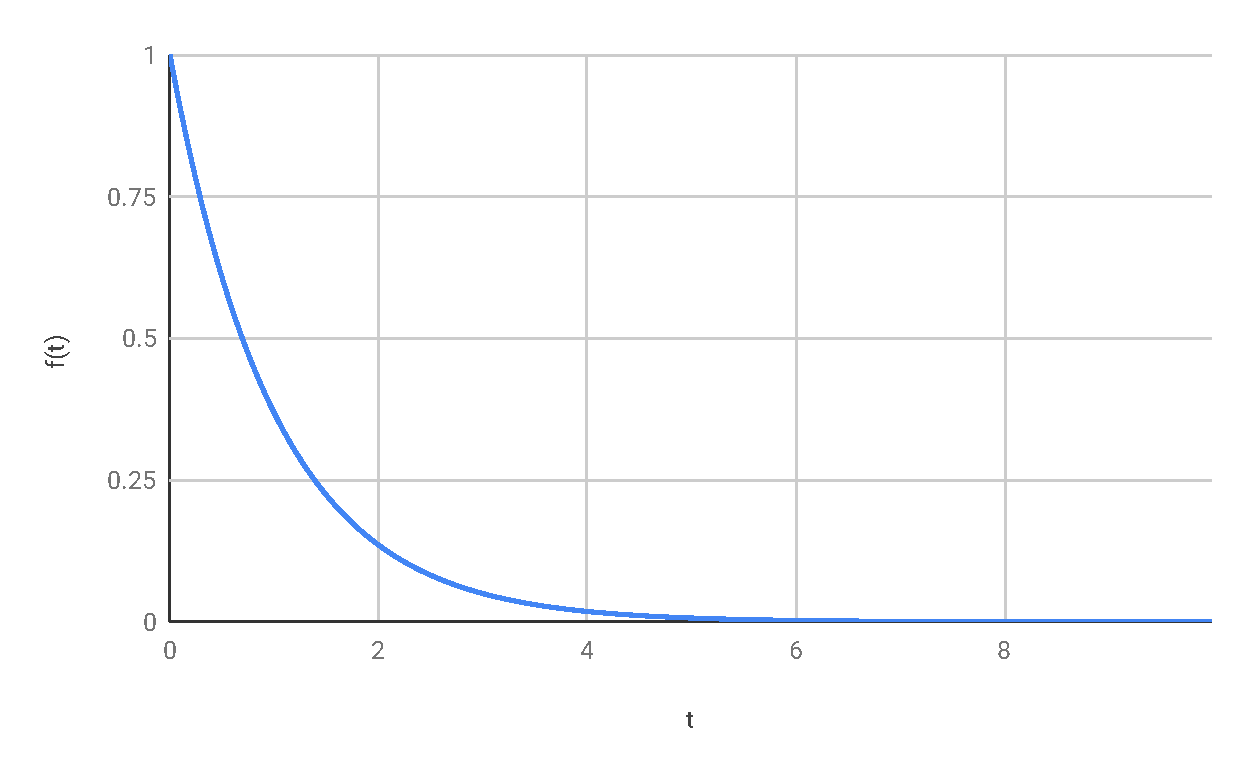
\includegraphics[scale=0.74]{image/05-RC-RL/f.pdf}
    \caption{Function $f(t)$}
    \label{figure.05.f}
\end{figure}
%%%%%%%%%%%%%%%%%%%%%%%%%%%%%%%%%%%%%%%%%%%%%%%%%%%%%%%%%%%%%%%%%%%%%%%%%%%%%%%%
\begin{figure}[ht]
    \centering
    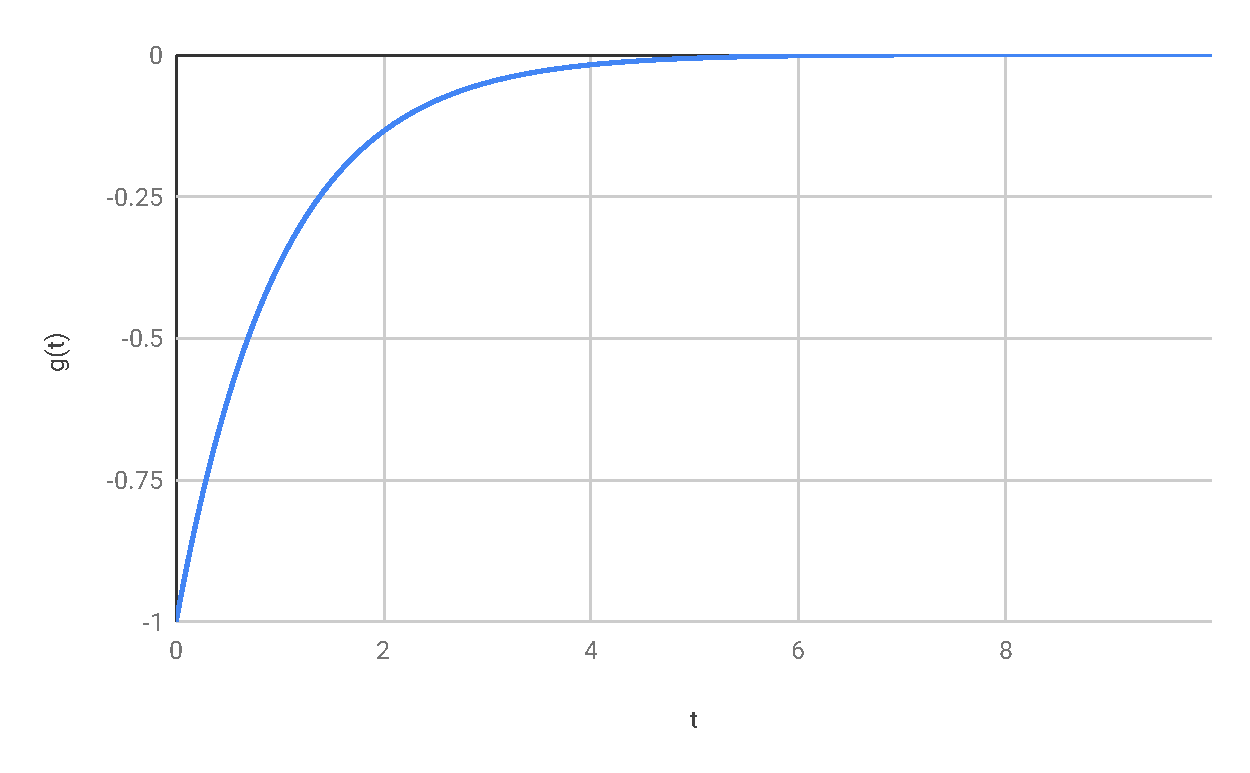
\includegraphics[scale=0.74]{image/05-RC-RL/g.pdf}
    \caption{Function $g(t)$}
    \label{figure.05.g}
\end{figure}
%%%%%%%%%%%%%%%%%%%%%%%%%%%%%%%%%%%%%%%%%%%%%%%%%%%%%%%%%%%%%%%%%%%%%%%%%%%%%%%%
\begin{figure}[ht]
    \centering
    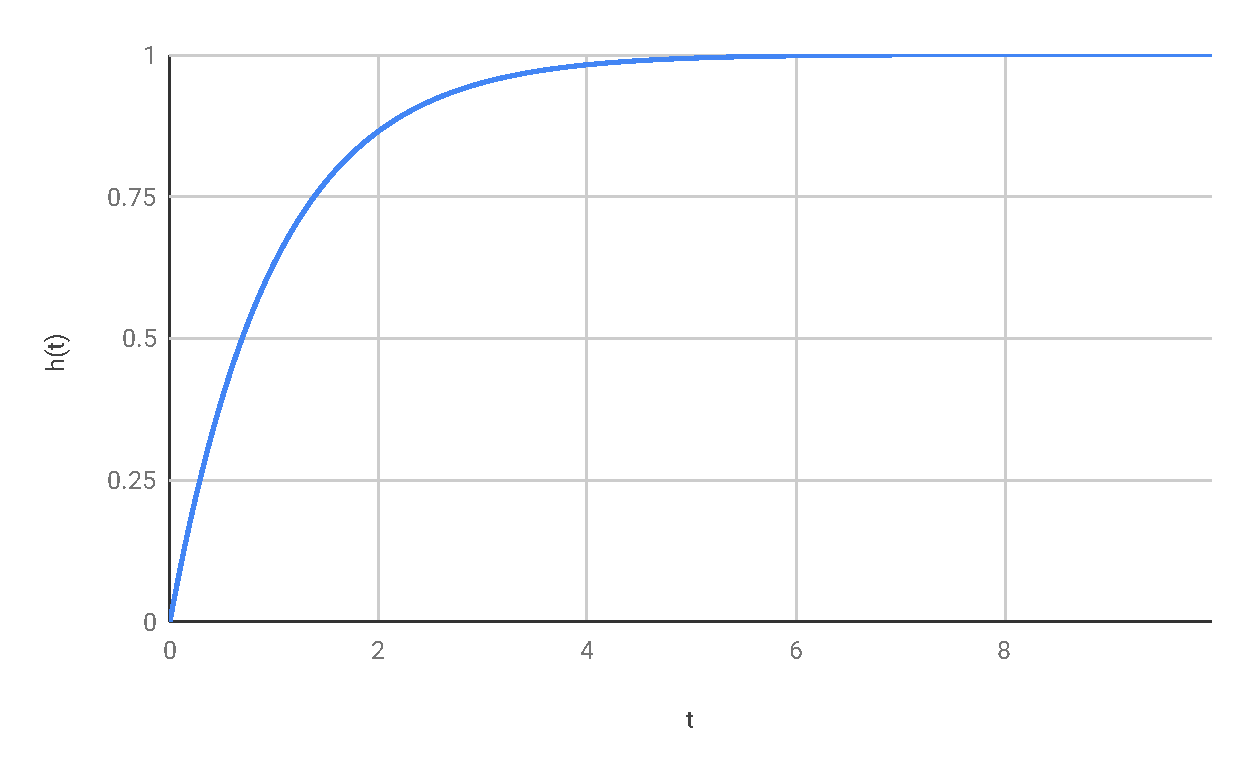
\includegraphics[scale=0.74]{image/05-RC-RL/h.pdf}
    \caption{Function $h(t)$}
    \label{figure.05.h}
\end{figure}
%%%%%%%%%%%%%%%%%%%%%%%%%%%%%%%%%%%%%%%%%%%%%%%%%%%%%%%%%%%%%%%%%%%%%%%%%%%%%%%%
\begin{figure}[ht]
    \centering
    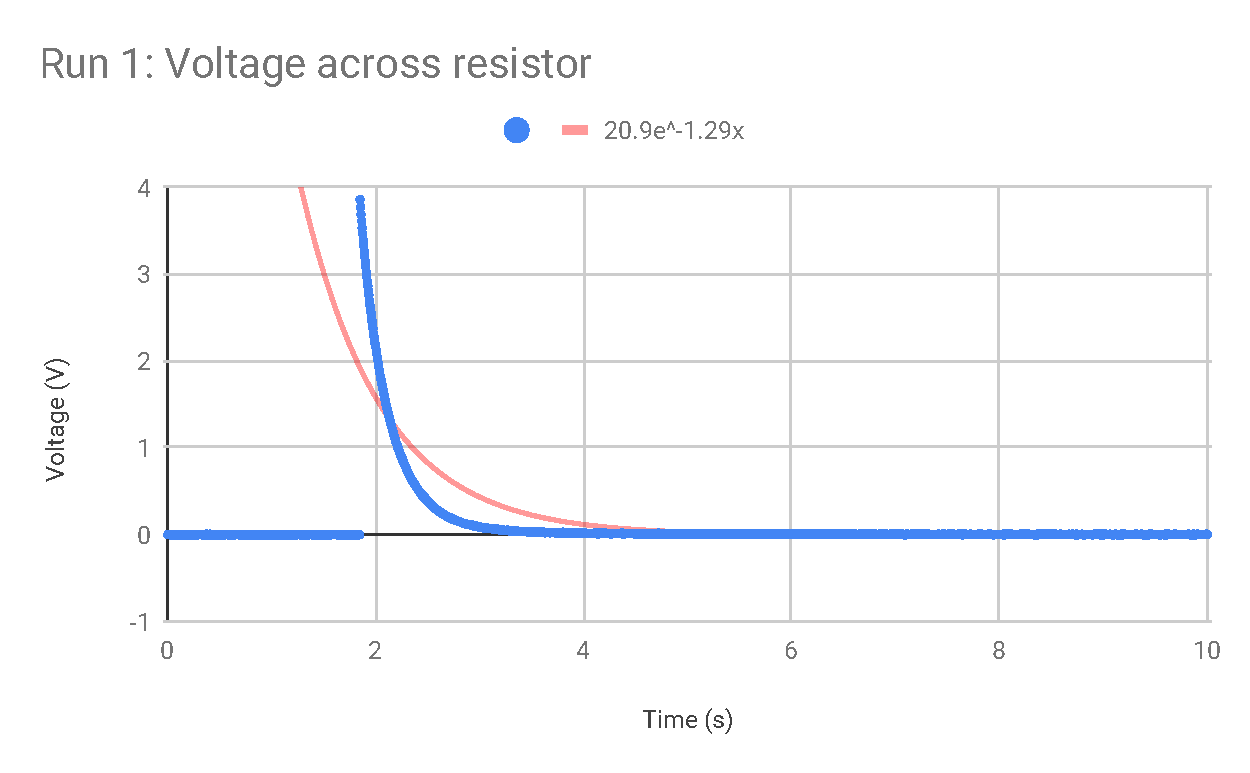
\includegraphics[scale=0.74]{image/05-RC-RL/run-1-vR-full.pdf}
    \caption{Run 1: $V_{R}(t)$}
    \label{figure.05.run.1.vR.full}
\end{figure}
%%%%%%%%%%%%%%%%%%%%%%%%%%%%%%%%%%%%%%%%%%%%%%%%%%%%%%%%%%%%%%%%%%%%%%%%%%%%%%%%
\begin{figure}[ht]
    \centering
    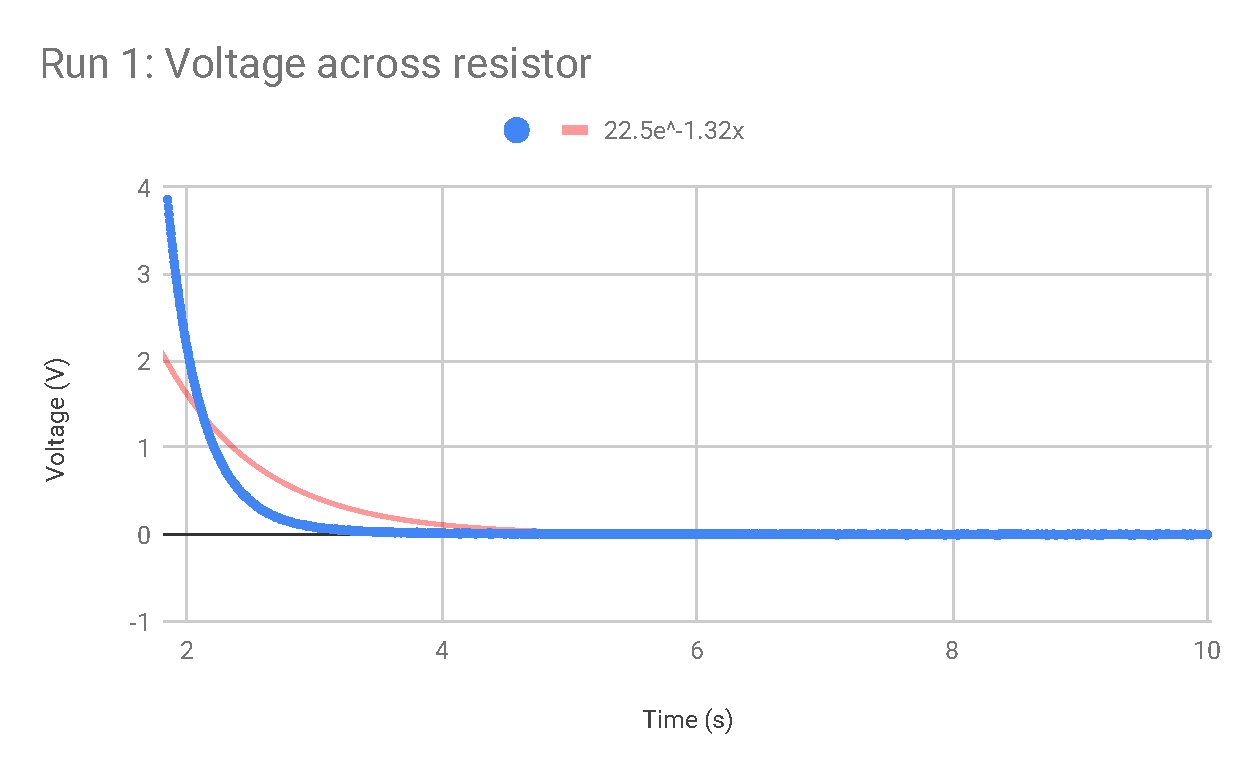
\includegraphics[scale=0.74]{image/05-RC-RL/run-1-vR-truncated.pdf}
    \caption{Run 1: $V_{R}(t)$}
    \label{figure.05.run.1.vR.truncated}
\end{figure}
%%%%%%%%%%%%%%%%%%%%%%%%%%%%%%%%%%%%%%%%%%%%%%%%%%%%%%%%%%%%%%%%%%%%%%%%%%%%%%%%
\begin{figure}[ht]
    \centering
    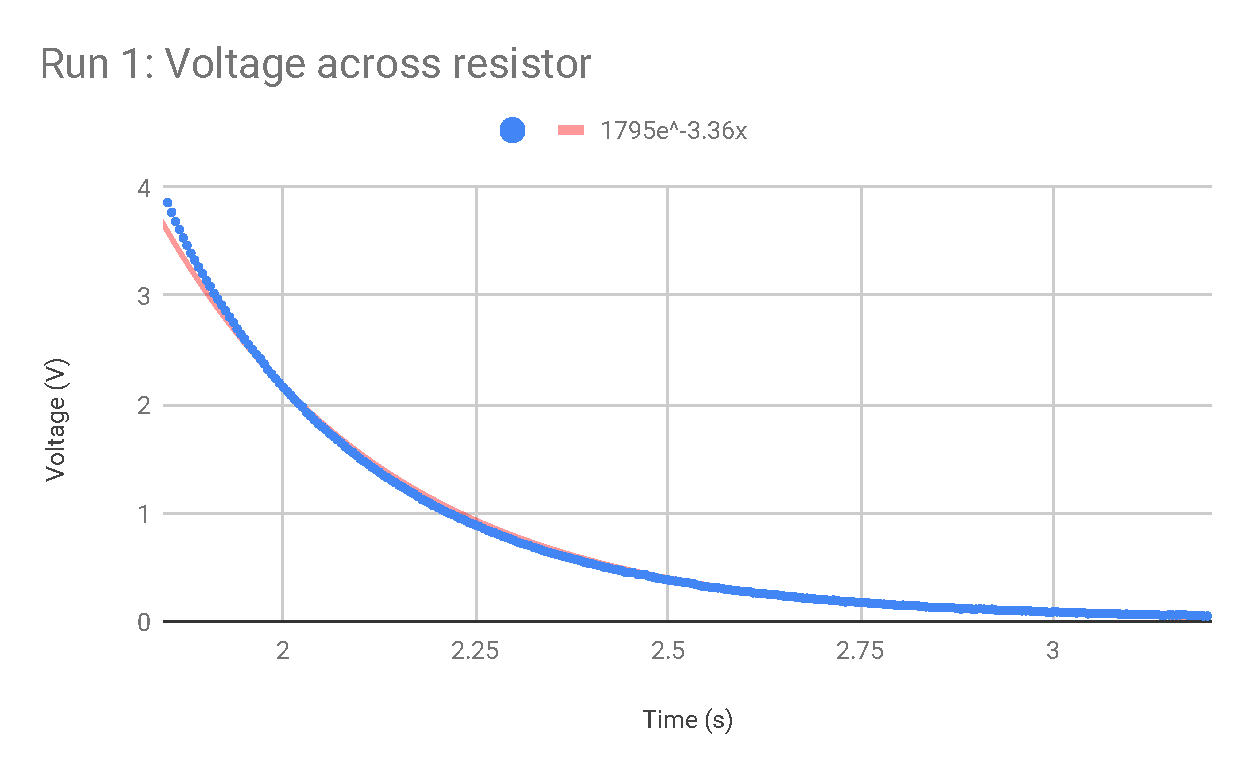
\includegraphics[scale=0.74]{image/05-RC-RL/run-1-vR-no-tail.pdf}
    \caption{Run 1: $V_{R}(t)$}
    \label{figure.05.run.1.vR.no.tail}
\end{figure}

% % Copyright 2018-2020 Melvin Eloy Irizarry-Gelpí
\setcounter{chapter}{4}
\chapter{Capacitors and Inductors}
%%%%%%%%%%%%%%%%%%%%%%%%%%%%%%%%%%%%%%%%%%%%%%%%%%%%%%%%%%%%%%%%%%%%%%%%%%%%%%%%
In this experiment you will learn about circuits with capacitors and inductors.
%%%%%%%%%%%%%%%%%%%%%%%%%%%%%%%%%%%%%%%%%%%%%%%%%%%%%%%%%%%%%%%%%%%%%%%%%%%%%%%%
\section{Preliminary}
%%%%%%%%%%%%%%%%%%%%%%%%%%%%%%%%%%%%%%%%%%%%%%%%%%%%%%%%%%%%%%%%%%%%%%%%%%%%%%%%
A given component in an electric circuit can have many physical properties. Among them are resistance, capacitance, and inductance.
%%%%%%%%%%%%%%%%%%%%%%%%%%%%%%%%%%%%%%%%%%%%%%%%%%%%%%%%%%%%%%%%%%%%%%%%%%%%%%%%
\subsection{Resistance and Resistors}
%%%%%%%%%%%%%%%%%%%%%%%%%%%%%%%%%%%%%%%%%%%%%%%%%%%%%%%%%%%%%%%%%%%%%%%%%%%%%%%%
By now, electrical \textbf{resistance} should be familiar. The \textbf{SI unit} for electrical resistance is the \textbf{ohm}:
\begin{equation}
	1 \text{ ohm} = 1\;\Omega = 1 \text{ V/A}
\end{equation}
Here, V is volt (voltage) and A is ampere (current). A component in a circuit with a fixed amount of resistance is called a \textbf{resistor}. The mathematical symbol for resistance is $R$.
%%%%%%%%%%%%%%%%%%%%%%%%%%%%%%%%%%%%%%%%%%%%%%%%%%%%%%%%%%%%%%%%%%%%%%%%%%%%%%%%
\subsection{Capacitance and Capacitors}
%%%%%%%%%%%%%%%%%%%%%%%%%%%%%%%%%%%%%%%%%%%%%%%%%%%%%%%%%%%%%%%%%%%%%%%%%%%%%%%%
Another important property is \textbf{capacitance}. The \textbf{SI unit} for capacitance is the \textbf{farad}:
\begin{equation}
	1 \text{ farad} = 1 \text{ F} = 1 \text{ C/V}
\end{equation}
Here, C is coulomb (electric charge) and V is volt (voltage). In some ways, capacitance measures the amount of electric charge needed to sustain an electric potential difference (i.e. a voltage). The mathematical symbol for capacitance is $C$.

A component in a circuit with a fixed amount of capacitance is called a \textbf{capacitor}. You can think of a capacitor as two parallel plates of conducting material where equal but opposite amounts of electric charge can accumulate.
%%%%%%%%%%%%%%%%%%%%%%%%%%%%%%%%%%%%%%%%%%%%%%%%%%%%%%%%%%%%%%%%%%%%%%%%%%%%%%%%
\subsection{Inductance and Inductors}
%%%%%%%%%%%%%%%%%%%%%%%%%%%%%%%%%%%%%%%%%%%%%%%%%%%%%%%%%%%%%%%%%%%%%%%%%%%%%%%%
The last property is \textbf{inductance}, which is like a magnetic cousin of capacitance. The \textbf{SI unit} for inductance is the \textbf{henry}:
\begin{equation}
	1 \text{ henry} = 1 \text{ H} = 1 \text{ T}\cdot\text{m}^{2}\text{/A}
\end{equation}
Here, T is tesla (magnetic field), m$^{2}$ is square meter (area), and A is ampere (current). Recall that the tesla unit is equivalent to
\begin{equation}
    1 \text{ T} = 1 \text{ V} \cdot \text{s/m}^{2}
\end{equation}
Thus, the henry unit is equivalent to:
\begin{equation}
    1 \text{ H} = 1 \text{ V}\cdot\text{s/A}
\end{equation}
In some ways, inductance measures the amount of voltage that arises per unit rate of change of electric current with time. The mathematical symbol for inductance is $L$.

A component in a circuit with a fixed amount of inductance is called an \textbf{inductor}. You can think of an inductor as a solenoid coil with a given amount of loops, with each loop enclosing some amount of area.
%%%%%%%%%%%%%%%%%%%%%%%%%%%%%%%%%%%%%%%%%%%%%%%%%%%%%%%%%%%%%%%%%%%%%%%%%%%%%%%%
\subsection{Exponential Decay Function}
%%%%%%%%%%%%%%%%%%%%%%%%%%%%%%%%%%%%%%%%%%%%%%%%%%%%%%%%%%%%%%%%%%%%%%%%%%%%%%%%
Before discussing the behavior of current and voltage in circuits with capacitors and inductors, it will be good to review the exponential decay function:
\begin{equation}
    \exp(-t) = e^{-t}
\end{equation}
Here, $e$ is the \textbf{natural base}:
\begin{equation}
    e = 2.71828...
\end{equation}
When $t = 0$, the exponential decay function gives
\begin{equation}
    \exp(0) = 1
\end{equation}
For large values of $t$, the exponential decay function approaches 0:
\begin{equation}
    \exp(-\infty) = 0
\end{equation}
In between $t = 0$ and $t \rightarrow \infty$ you have smaller and smaller values approaching zero.

The exponential decay function is an example of a function that is always positive, and always \textbf{decreasing} towards zero:
\begin{align}
    f(t) = \exp(-t) && 0 < f(t) \leq 1 && 0 \leq t < \infty
\end{align}
Multiplying the exponential decay function by a negative sign produces a function that is always negative, and always \textbf{increasing} towards zero:
\begin{align}
    g(t) = -\exp(-t) && -1 \leq g(t) < 0 && 0 \leq t < \infty
\end{align}
Another important combination is shifting vertically by 1, which gives a function that is always positive, and always \textbf{increasing} towards one:
\begin{align}
    h(t) = 1 - \exp(-t) && 0 \leq h(t) < 1 && 0 \leq t < \infty
\end{align}
Figures \ref{figure.05.f}, \ref{figure.05.g}, and \ref{figure.05.h} provide charts for these three functions.
%%%%%%%%%%%%%%%%%%%%%%%%%%%%%%%%%%%%%%%%%%%%%%%%%%%%%%%%%%%%%%%%%%%%%%%%%%%%%%%%
\subsection{Resistor and Capacitor in Series}
%%%%%%%%%%%%%%%%%%%%%%%%%%%%%%%%%%%%%%%%%%%%%%%%%%%%%%%%%%%%%%%%%%%%%%%%%%%%%%%%
A circuit with a resistor, a capacitor, and a direct-current (DC) source is called an \textbf{RC circuit}. In the simplest RC circuit, the resistor and capacitor are connected in series to the DC source via a particular switch.
%%%%%%%%%%%%%%%%%%%%%%%%%%%%%%%%%%%%%%%%%%%%%%%%%%%%%%%%%%%%%%%%%%%%%%%%%%%%%%%%
\subsubsection{Charging the Capacitor}
%%%%%%%%%%%%%%%%%%%%%%%%%%%%%%%%%%%%%%%%%%%%%%%%%%%%%%%%%%%%%%%%%%%%%%%%%%%%%%%%
When the switch is on, and the circuit is complete, the DC source pushes charges out into the circuit in the form of a current. This current causes positive electric charges to accumulate on one of the terminals of the capacitor, and negative electric charges on the other terminal of the capacitor. But the amount of electric charge $Q$ on the capacitor does not increase indefinitely: It settles on a maximum value $Q_{\infty}$. The particular manner in which the amount of \textbf{electric charge} on the capacitor increases with time is an example of an \textbf{exponential} increase:
\begin{equation}
    Q(t) = Q_{\infty} \left[ 1 - \exp\left(-\frac{t}{\tau_{C}}\right) \right]
    \label{eq.05.RC.q.charging}
\end{equation}
Here $Q_{\infty}$ is the amount of charge accumulated on the capacitor after an infinite amount of time, and $t$ correspond to the amount of time after the switch has been opened (the switch is opened at $t = 0$). The amount of \textbf{current} corresponds to the rate of change of the electric charge with time:
\begin{equation}
    I(t) = I_{0} \exp\left(-\frac{t}{\tau_{C}}\right)
    \label{eq.05.RC.i.charging}
\end{equation}
For a capacitor with capacitance $C$, the amount of \textbf{voltage} $V_{C}$ across the \textbf{capacitor} is directly proportional to the amount of electric charge accumulated on the capacitor:
\begin{equation}
    V_{C}(t) = \frac{Q(t)}{C} = V_{\infty} \left[ 1 - \exp\left(-\frac{t}{\tau_{C}}\right) \right]
    \label{eq.05.RC.vC.charging}
\end{equation}
The \textbf{voltage} $V_{R}$ across the \textbf{resistor} is directly proportional the the amount of current, via Ohm's law:
\begin{equation}
    V_{R}(t) = R I(t) = V_{\infty} \exp\left(-\frac{t}{\tau_{C}}\right)
    \label{eq.05.RC.vR.charging}
\end{equation}
Here, $V_{\infty}$ is related to $Q_{\infty}$ and/or $I_{0}$ via
\begin{eqnarray}
    V_{\infty} = \frac{Q_{\infty}}{C} = I_{0} R
\end{eqnarray}
The value of $V_{\infty}$ should correspond to the steady voltage across the DC source.

As you can see from (\ref{eq.05.RC.q.charging}), (\ref{eq.05.RC.i.charging}), and (\ref{eq.05.RC.vC.charging}), the amount of charge, current and voltage related to a capacitor all involve exponential functions. The constant $\tau_{C}$ is known as the \textbf{capacitive time constant}. It has units of time (seconds). The value of $\tau_{C}$ sets a time scale for the change in values to occur. The same time scale appears in all three quantities. In an RC circuit, the value of $\tau_{C}$ depends on how much resistance $R$ and capacitance $C$ you have:
\begin{equation}
    \tau_{C} = R C
    \label{eq.05.tauC}
\end{equation}
You can check that, in fact, by multiplying something with ohm units by something with farad units you get something with second units:
\begin{equation}
    1 \text{ ohm} \cdot 1 \text{ F} = \left(1 \text{ V}\cdot\text{ s/C}\right) \cdot \left(1 \text{ C/V}\right) = 1 \text{ s}
\end{equation}
Since the exponential function is a mathematical function that changes very fast, the current will take noise-level values after a time corresponding to about 5 capacitive time constants.
%%%%%%%%%%%%%%%%%%%%%%%%%%%%%%%%%%%%%%%%%%%%%%%%%%%%%%%%%%%%%%%%%%%%%%%%%%%%%%%%
\subsubsection{Discharging the Capacitor}
%%%%%%%%%%%%%%%%%%%%%%%%%%%%%%%%%%%%%%%%%%%%%%%%%%%%%%%%%%%%%%%%%%%%%%%%%%%%%%%%
After some time with the switch on, the amount of charge on the capacitor becomes almost constant (close to $Q_{\infty}$), the amount of voltage across the capacitor also becomes almost constant (close to $V_{\infty}$), and the current through the circuit becomes almost zero. Upon opening the circuit by setting the switch off, the DC source stops supporting the charge accumulated on the capacitor, and that amount of charge begins to leave the capacitor. The amount of charge on the capacitor follows a particular manner:
\begin{equation}
    Q(t) = Q_{0} \exp\left(-\frac{t}{\tau_{C}}\right)
    \label{eq.05.RC.q.discharging}
\end{equation}
Here $Q_{0}$ is the amount of charge at the moment that the switch is turned off. The electric current is given by
\begin{equation}
    I(t) = - I_{0} \exp\left(-\frac{t}{\tau_{C}}\right)
    \label{eq.05.RC.i.discharging}
\end{equation}
This behavior is very similar to the behavior of the current (\ref{eq.05.RC.i.charging}) while the capacitor is charging, except that the negative sign indicates the current is in the opposite direction, since the charge is leaving the capacitor. The voltage $V_{C}$ across the \textbf{capacitor} can, again, be found from the amount of electric charge:
\begin{equation}
    V_{C}(t) = \frac{Q(t)}{C} = V_{0} \exp\left(-\frac{t}{\tau_{C}}\right)
    \label{eq.05.RC.vC.discharging}
\end{equation}
The capacitive time constant appears again, and also dictates the time scale for the decrease of the charge, current and voltage across the capacitor during the discharging event. The voltage $V_{R}$ across the \textbf{resistor} can, again, be found from the amount of electric current:
\begin{equation}
    V_{R}(t) = R I(t) = - V_{0} \exp\left(-\frac{t}{\tau_{C}}\right)
\end{equation}
Just as before, there is a relation between $Q_{0}$, $I_{0}$, and $V_{0}$:
\begin{equation}
    V_{0} = \frac{Q_{0}}{C} = I_{0} R
\end{equation}
The value of $V_{0}$ should correspond to the voltage across the capacitor just before the switch is opened.
%%%%%%%%%%%%%%%%%%%%%%%%%%%%%%%%%%%%%%%%%%%%%%%%%%%%%%%%%%%%%%%%%%%%%%%%%%%%%%%%
\subsection{Resistor and Inductor in Series}
%%%%%%%%%%%%%%%%%%%%%%%%%%%%%%%%%%%%%%%%%%%%%%%%%%%%%%%%%%%%%%%%%%%%%%%%%%%%%%%%
A circuit with a resistor, an inductor, and a DC source is called an \textbf{RL circuit}. In the simplest RL circuit, the resistor and inductor are connected in series to the DC source via a particular switch.

An \textbf{ideal inductor} is an inductor that has \textbf{zero electrical resistance}. In practice, the inductors that you will use in these experiments have a non-negligible amount of resistance that cannot be ignored and has to be taken into account. One way to do this is to think of a \textbf{non-ideal inductor} as consisting of a resistor and an ideal inductor connected in series:
\begin{equation}
    \text{non-ideal inductor} = \text{resistor} + \text{ideal inductor in series}
\end{equation}
Thus, an RL circuit with one resistor with resistance $R$ and one non-ideal inductor with resistance $r$ and inductance $L$ in series is equivalent to an RL circuit with \textbf{two} resistors and one ideal inductor in series. Let $V_{0}$ correspond to the EMF voltage produced by the DC source in the RL circuit. Then, since the circuit is in series, the amount of EMF voltage from the DC source must be equivalent to the sum of voltages across the two resistors and the ideal inductor:
\begin{equation}
    V_{0} = V_{R} + V_{r} + V_{L}
\end{equation}
Here, $V_{R}$ is the voltage across the main resistor, $V_{r}$ is the voltage across the resistor with the inductor resistance, and $V_{L}$ is the voltage across the ideal inductor. The problem is that you can directly measure $V_{R}$, but not $V_{L}$. Instead, measuring the voltage across the inductor gives the non-ideal total $V_{r} + V_{L}$. The other problem is that $V_{L}$ is what you really want, so $V_{r}$ has to be subtracted from the inductor measurement.

Although an inductor does not accumulate electric charge like a capacitor, the behavior of electric current and voltage across an inductor in an RL circuit also involves \textbf{exponential} functions.

Whereas in an RC circuit the current becomes zero for large time values after closing the switch, in an RL circuit the current rises to a steady value:
\begin{equation}
    I(t) = I_{\infty} \left[ 1 - \exp\left(- \frac{t}{\tau_{L}}\right) \right]
    \label{eq.05.RL.i.rise}
\end{equation}
The \textbf{voltage} $V_{R}$ across the main \textbf{resistor} is given by Ohm's law:
\begin{equation}
    V_{R}(t) = R I(t) = R I_{\infty} \left[ 1 - \exp\left(- \frac{t}{\tau_{L}}\right) \right]
    \label{eq.05.RL.vR}
\end{equation}
The \textbf{voltage} $V_{r}$ across the second resistor is also given by Ohm's law:
\begin{equation}
    V_{r}(t) = r I(t) = r I_{\infty} \left[ 1 - \exp\left(- \frac{t}{\tau_{L}}\right) \right]
    \label{eq.05.RL.vr}
\end{equation}
The \textbf{voltage} $V_{L}$ across the \textbf{inductor} is given by
\begin{equation}
    V_{L}(t) = V_{0} - V_{R}(t) - V_{r}(t) = V_{0} \exp\left(- \frac{t}{\tau_{L}}\right)
    \label{eq.05.RL.vL}
\end{equation}
Here $I_{\infty}$ and $V_{0}$ are related via
\begin{equation}
    V_{0} = I_{\infty} \left(R + r\right)
\end{equation}
Instead of $\tau_{C}$, you now have $\tau_{L}$ which corresponds to the \textbf{inductive time constant}. Just like $\tau_{C}$, the value of $\tau_{L}$ depends on the total amount of resistance and also on the inductance you have in the circuit:
\begin{equation}
    \tau_{L} = \frac{L}{R + r}
    \label{eq.05.tauL}
\end{equation}
You can check that in fact, by dividing something with henry units by something with ohm units you get something with second units.
%%%%%%%%%%%%%%%%%%%%%%%%%%%%%%%%%%%%%%%%%%%%%%%%%%%%%%%%%%%%%%%%%%%%%%%%%%%%%%%%
\section{Experiment}
%%%%%%%%%%%%%%%%%%%%%%%%%%%%%%%%%%%%%%%%%%%%%%%%%%%%%%%%%%%%%%%%%%%%%%%%%%%%%%%%
You did experiments for both RC and RL circuits.
%%%%%%%%%%%%%%%%%%%%%%%%%%%%%%%%%%%%%%%%%%%%%%%%%%%%%%%%%%%%%%%%%%%%%%%%%%%%%%%%
\subsection{RC Circuits}
%%%%%%%%%%%%%%%%%%%%%%%%%%%%%%%%%%%%%%%%%%%%%%%%%%%%%%%%%%%%%%%%%%%%%%%%%%%%%%%%
For RC circuits there are two kinds of events: the \textbf{charging} event and the \textbf{discharging} event. In each experiment you measured
\begin{itemize}
    \item the voltage across the \textbf{resistor}, $V_{R}(t)$;
    \item the current flowing between the resistor and the capacitor, $I(t)$; and
    \item the voltage across the \textbf{capacitor}, $V_{C}(t)$.
\end{itemize}
For the \textbf{charging event}, the data collection was started with the switch off (i.e. incomplete circuit) and shortly after turned on. You should analyze the \textbf{current} and the \textbf{voltage across the resistor} for such events.

For the \textbf{discharging event}, the data collection was started with the switch on (i.e. complete circuit) and shortly after turned off. You should analyze the \textbf{voltage across the capacitor} for such events.

There are many resistors and capacitors available. Each time the resistance or the capacitance changes, the time constant $\tau_{C}$ will also change.
%%%%%%%%%%%%%%%%%%%%%%%%%%%%%%%%%%%%%%%%%%%%%%%%%%%%%%%%%%%%%%%%%%%%%%%%%%%%%%%%
\subsection{RL Circuits}
%%%%%%%%%%%%%%%%%%%%%%%%%%%%%%%%%%%%%%%%%%%%%%%%%%%%%%%%%%%%%%%%%%%%%%%%%%%%%%%%
For RL circuits, all the experiments involved closing the switch after the data collection was started. You measured
\begin{itemize}
    \item the voltage across the resistor, $V_{R}(t)$;
    \item the current flowing between the resistor and the non-ideal inductor, $I(t)$; and
    \item the voltage across the non-ideal inductor. $V_{r}(t) + V_{L}(t)$.
\end{itemize}
Because the inductive time constants are so small, the data acquisition needs to be activated with the trigger feature.

The inductors come with a \textbf{metallic core}. Each experiment is done twice: Once without the core, and once with the core. The effect of the core is to change the inductance of the inductor.

There are many resistors, and many ways to connect inductors of the same type. Each time the resistance or the inductance changes, the time constant $\tau_{L}$ will also change.
%%%%%%%%%%%%%%%%%%%%%%%%%%%%%%%%%%%%%%%%%%%%%%%%%%%%%%%%%%%%%%%%%%%%%%%%%%%%%%%%
\section{Analysis}
%%%%%%%%%%%%%%%%%%%%%%%%%%%%%%%%%%%%%%%%%%%%%%%%%%%%%%%%%%%%%%%%%%%%%%%%%%%%%%%%
The common feature of $f(t)$, $g(t)$, and $h(t)$ above is that they all settle on steady values for infinite time after $t = 0$. In an experiment, you do not have an infinite amount of time, so a relevant question is how long corresponds to infinite time. Since you are using imperfect sensors to measure current and voltage, after some time of decreasing towards zero, there will be a point where measurements are not distinguishable from noise.

Consider the following function:
\begin{equation}
    A(t) = A_{0} \exp\left(- \frac{t}{\tau}\right)
\end{equation}
At $t = 0$, you have
\begin{equation}
    A(0) = A_{0}
\end{equation}
Thus, $A_{0}$ correspond to the amount of $A$ present at $t = 0$. The value of $A$ after one unit of $\tau$ is:
\begin{equation}
    A(\tau) = A_{0} \exp\left(-1\right) = 0.3679 \cdot A_{0}
\end{equation}
That is, about 37\% of the starting value. After two units of $\tau$ you have:
\begin{equation}
    A(2\tau) = A_{0} \exp\left(-2\right) = 0.1353 \cdot A_{0}
\end{equation}
That is, about 14\% of the starting value. After three units of $\tau$ you have:
\begin{equation}
    A(3\tau) = A_{0} \exp\left(-3\right) = 0.0498 \cdot A_{0}
\end{equation}
That is, about 5\% of the starting value. After four units of $\tau$ you have:
\begin{equation}
    A(4\tau) = A_{0} \exp\left(-4\right) = 0.0183 \cdot A_{0}
\end{equation}
That is, about 2\% of the starting value. After five units of $\tau$ you have:
\begin{equation}
    A(5\tau) = A_{0} \exp\left(-5\right) = 0.0067 \cdot A_{0}
\end{equation}
That is, about 0.67\% of the starting value. Five units of $\tau$ is a good rule of thumb. In principle, the quantity that is being measured will continue decreasing in value, but in practice those small values cannot be reliably measured. If you have an estimate of the amount of $\tau$, then from the time the decay begins you should unlike keep until after $5 \tau$ has passed.
%%%%%%%%%%%%%%%%%%%%%%%%%%%%%%%%%%%%%%%%%%%%%%%%%%%%%%%%%%%%%%%%%%%%%%%%%%%%%%%%
\subsection{RC Circuits: Charging Events}
%%%%%%%%%%%%%%%%%%%%%%%%%%%%%%%%%%%%%%%%%%%%%%%%%%%%%%%%%%%%%%%%%%%%%%%%%%%%%%%%
In a charging even both the voltage across the resistor and the current decay exponentially. Here are some steps to follow:
%%%%%%%%%%%%%%%%%%%%%%%%%%%%%%%%%%%%%%%%%%%%%%%%%%%%%%%%%%%%%%%%%%%%%%%%%%%%%%%%
\subsubsection{Visualize $V_{R}$ and $I$}
%%%%%%%%%%%%%%%%%%%%%%%%%%%%%%%%%%%%%%%%%%%%%%%%%%%%%%%%%%%%%%%%%%%%%%%%%%%%%%%%
Make two scatter charts:
\begin{itemize}
    \item Voltage across the resistor in the vertical axis, and time in the horizontal axis.
    \item Current in the vertical axis, and time in the horizontal axis.
\end{itemize}
You might want to add exponential fits, although at this stage they would most likely not be appropriate. See Figure \ref{figure.05.run.1.vR.full} for an example.
%%%%%%%%%%%%%%%%%%%%%%%%%%%%%%%%%%%%%%%%%%%%%%%%%%%%%%%%%%%%%%%%%%%%%%%%%%%%%%%%
\subsubsection{Truncate the part before closing circuit}
%%%%%%%%%%%%%%%%%%%%%%%%%%%%%%%%%%%%%%%%%%%%%%%%%%%%%%%%%%%%%%%%%%%%%%%%%%%%%%%%
Before the exponential fit can be made meaningful, you need to truncate the part of the data before the switch is closed. Looking at the columns, it should be obvious when the values for $V_{R}$ and $I$ suddenly take large values. See Figure \ref{figure.05.run.1.vR.truncated} for an example after truncation.
%%%%%%%%%%%%%%%%%%%%%%%%%%%%%%%%%%%%%%%%%%%%%%%%%%%%%%%%%%%%%%%%%%%%%%%%%%%%%%%%
\subsubsection{Truncate the long tail}
%%%%%%%%%%%%%%%%%%%%%%%%%%%%%%%%%%%%%%%%%%%%%%%%%%%%%%%%%%%%%%%%%%%%%%%%%%%%%%%%
It is very likely that after removing the part of the data before closing the circuit, the exponential fit might still not be appropriate. If the decay is relatively quick, and the voltage or current has a long segment where it is just zero, that long tail section will skew the fit process and render incorrect results. For this reason, it is good to only keep a time segment that is about $5\tau_{C}$ long. For example, after truncation in Figure \ref{figure.05.run.1.vR.truncated}, the decay begins around $t = 1.85$ seconds. For this particular run, the expected value of the time constant is $\tau_{C} = 0.250$ seconds. Thus,
\begin{equation}
    1.85 \text{ s} + 5 \tau_{C} = 3.10 \text{ s}
\end{equation}
All the data after $t = 3.10$ seconds should be truncated also. For good measure, I am keeping everything up to $t = 3.20$ seconds. See Figure \ref{figure.05.run.1.vR.no.tail} for an example.
%%%%%%%%%%%%%%%%%%%%%%%%%%%%%%%%%%%%%%%%%%%%%%%%%%%%%%%%%%%%%%%%%%%%%%%%%%%%%%%%
\subsubsection{Extract the experimental value of $\tau_{C}$}
%%%%%%%%%%%%%%%%%%%%%%%%%%%%%%%%%%%%%%%%%%%%%%%%%%%%%%%%%%%%%%%%%%%%%%%%%%%%%%%%
After truncating the initial and long tail parts, the exponential fit should be appropriate for the data. The exponential fit is given in the form
\begin{equation}
    a \exp(-bx)
\end{equation}
The value of $b$ corresponds to the inverse of the time constant:
\begin{equation}
    b = \frac{1}{\tau_{C}}
\end{equation}
Thus, the observed value of the time constant follows from the inverse of $b$:
\begin{equation}
    \text{Observed } \tau_{C} = \frac{1}{b}
\end{equation}
You should get a value from the $V_{R}$ chart, and another value from the $I$ chart. Both values should be consistent with each other.
%%%%%%%%%%%%%%%%%%%%%%%%%%%%%%%%%%%%%%%%%%%%%%%%%%%%%%%%%%%%%%%%%%%%%%%%%%%%%%%%
\subsection{RC Circuits: Discharging Events}
%%%%%%%%%%%%%%%%%%%%%%%%%%%%%%%%%%%%%%%%%%%%%%%%%%%%%%%%%%%%%%%%%%%%%%%%%%%%%%%%
In the discharging event, only the voltage across the capacitor follows an exponential decay. The steps are similar:
\begin{enumerate}
    \item Visualize the data with a scatter chart with the voltage across the capacitor in the vertical axis, and time in the horizontal axis.
    \item Truncate the part before opening the circuit.
    \item Truncate the long tail and keep close to $5\tau_{C}$ after the time the decay begins.
    \item Extract the experimental value of $\tau_{C}$ from the fit equation.
\end{enumerate}
The value of $\tau_{C}$ for the discharging even should be consistent with the value for the charging event.
%%%%%%%%%%%%%%%%%%%%%%%%%%%%%%%%%%%%%%%%%%%%%%%%%%%%%%%%%%%%%%%%%%%%%%%%%%%%%%%%
\subsection{RL Circuits: Resistance of Inductors}
%%%%%%%%%%%%%%%%%%%%%%%%%%%%%%%%%%%%%%%%%%%%%%%%%%%%%%%%%%%%%%%%%%%%%%%%%%%%%%%%
Before dealing with the inductive time constant experiments, you have to determine how much electrical resistance does the non-ideal inductors that are available have. Just like for resistors, in order to measure resistance you obtain current and voltage data over time. Using
\begin{equation}
    r = \frac{V_{r}(t)}{I(t)}
\end{equation}
should provide the observed value of the resistance of the non-ideal inductor over time. This value should be steady and almost constant, so take a time average to get the best estimate.

For two non-ideal inductors in series, you should find that the resistance is close to double the resistance for a single non-ideal inductor in series. 
%%%%%%%%%%%%%%%%%%%%%%%%%%%%%%%%%%%%%%%%%%%%%%%%%%%%%%%%%%%%%%%%%%%%%%%%%%%%%%%%
\subsection{RL Circuits: Inductive Time Constant}
%%%%%%%%%%%%%%%%%%%%%%%%%%%%%%%%%%%%%%%%%%%%%%%%%%%%%%%%%%%%%%%%%%%%%%%%%%%%%%%%
For these experiments you measured the voltage $V_{R}(t)$ across the resistor, the current $I(t)$ between the resistor and the non-ideal inductor, and the voltage $V_{r}(t) + V_{L}(t)$ across the non-ideal inductor.

As Figure \ref{figure.05.vL.nonideal.full} shows, the voltage across the non-ideal inductor does not decay exponentially. The only quantity that decays exponentially is the voltage $V_{L}(t)$ across the ideal inductor. In order to obtain this, you have to subtract the voltage $V_{r}(t)$ due to the resistance of the non-ideal inductor from the signal. The voltage due to the resistance of the inductor is given by
\begin{equation}
    V_{r}(t) = r I(t)
\end{equation}
Here, $r$ is the resistance of the non-ideal inductor. You measured this in the previous section. You should calculate this in a separate column, and then subtract this from the column with the voltage across the non-ideal inductor. After this subtraction, the data should show an exponential decay curve that approaches zero. See Figure \ref{figure.05.vL.full}. After removing the long tail, the exponential fit becomes appropriate. See Figure \ref{figure.05.run.1.vL}.
%%%%%%%%%%%%%%%%%%%%%%%%%%%%%%%%%%%%%%%%%%%%%%%%%%%%%%%%%%%%%%%%%%%%%%%%%%%%%%%%
\section{My Data}
%%%%%%%%%%%%%%%%%%%%%%%%%%%%%%%%%%%%%%%%%%%%%%%%%%%%%%%%%%%%%%%%%%%%%%%%%%%%%%%%
For the RC circuits, my data consist of twelve runs:
\begin{itemize}
    \item Run 1: Charging capacitor with $R = 10$ ohm and $C = 2.5 \times 10^{-2}$ F.
	\item Run 2: Discharging capacitor with $R = 10$ ohm and $C = 2.5 \times 10^{-2}$ F.
	\item Run 3: Charging capacitor with $R = 51$ ohm and $C = 2.5 \times 10^{-2}$ F.
	\item Run 4: Discharging capacitor with $R = 51$ ohm and $C = 2.5 \times 10^{-2}$ F.
	\item Run 5: Charging capacitor with $R = 68$ ohm and $C = 2.5 \times 10^{-2}$ F.
	\item Run 6: Discharging capacitor with $R = 68$ ohm and $C = 2.5 \times 10^{-2}$ F.
	\item Run 7: Charging capacitor with $R = 4.7 \times 10^{4}$ ohm and $C = 10^{-5}$ F.
	\item Run 8: Discharging capacitor with $R = 4.7 \times 10^{4}$ ohm and $C = 10^{-5}$ F.
	\item Run 9: Charging capacitor with $R = 10^{5}$ ohm and $C = 10^{-5}$ F.
	\item Run 10: Discharging capacitor with $R = 10^{5}$ ohm and $C = 10^{-5}$ F.
	\item Run 11: Charging capacitor with $R = 2.2 \times 10^{4}$ ohm and $C = 10^{-5}$ F.
	\item Run 12: Discharging capacitor with $R = 2.2 \times 10^{4}$ ohm and $C = 10^{-5}$ F.
\end{itemize}
For the RL circuits, my data consist of eight runs:
\begin{itemize}
    \item Run 1: $R = 10$ ohm, one inductor without metallic core ($L = 0.005$ H).
    \item Run 2: $R = 10$ ohm, one inductor with metallic core (unknown $L$).
    \item Run 3: $R = 5$ ohm, one inductor without metallic core ($L = 0.005$ H).
    \item Run 4: $R = 5$ ohm, one inductor with metallic core (unknown $L$).
    \item Run 5: $R = 10$ ohm, two inductors without metallic core ($L = 0.01$ H).
    \item Run 6: $R = 10$ ohm, two inductors with metallic core (unknown $L$).
    \item Run 7: $R = 5$ ohm, two inductors without metallic core ($L = 0.01$ H).
    \item Run 8: $R = 5$ ohm, two inductors with metallic core (unknown $L$).
\end{itemize}
%%%%%%%%%%%%%%%%%%%%%%%%%%%%%%%%%%%%%%%%%%%%%%%%%%%%%%%%%%%%%%%%%%%%%%%%%%%%%%%%
\subsection{RC Circuits}
%%%%%%%%%%%%%%%%%%%%%%%%%%%%%%%%%%%%%%%%%%%%%%%%%%%%%%%%%%%%%%%%%%%%%%%%%%%%%%%%
My results for the RC circuits are summarize in Table \ref{table.05.results.tauC.VR}, Table \ref{table.05.results.tauC.I}, and Table \ref{table.05.results.tauC.VC}. As you can see, the results are consistent with each other, and somewhat consistent with the expected value of the capacitive time constant. Indeed, when the resistance is increased, the observed time constant also increases. It is interesting that the results from the voltage across the resistor are not as accurate as the results for the voltage across the capacitor.
%%%%%%%%%%%%%%%%%%%%%%%%%%%%%%%%%%%%%%%%%%%%%%%%%%%%%%%%%%%%%%%%%%%%%%%%%%%%%%%%
\subsection{RL Circuits}
%%%%%%%%%%%%%%%%%%%%%%%%%%%%%%%%%%%%%%%%%%%%%%%%%%%%%%%%%%%%%%%%%%%%%%%%%%%%%%%%
The results for the inductive time constant from the voltage across the ideal inductor are in Table \ref{table.05.results.tauL.VL}. As you can see, the effect of using the metallic core is to increase the inductance. When you decrease the resistance, the time constant becomes larger.
%%%%%%%%%%%%%%%%%%%%%%%%%%%%%%%%%%%%%%%%%%%%%%%%%%%%%%%%%%%%%%%%%%%%%%%%%%%%%%%%
\section{Your Data}
%%%%%%%%%%%%%%%%%%%%%%%%%%%%%%%%%%%%%%%%%%%%%%%%%%%%%%%%%%%%%%%%%%%%%%%%%%%%%%%%
For the RC circuits, your data will consist of the following runs:
\begin{itemize}
    \item Run 1: Charging capacitor with $R = 10$ ohm and $C = 2.5 \times 10^{-2}$ F.
	\item Run 2: Discharging capacitor with $R = 10$ ohm and $C = 2.5 \times 10^{-2}$ F.
	\item Run 3: Charging capacitor with either $R = 51$ ohm or $R = 68$ ohm and $C = 2.5 \times 10^{-2}$ F.
	\item Run 4: Discharging capacitor with either $R = 51$ ohm or $R = 68$ ohm and $C = 2.5 \times 10^{-2}$ F.
	\item Run 5: Charging capacitor with either $R = 2.2 \times 10^{4}$ ohm or $R = 4.7 \times 10^{4}$ ohm and $C = 10^{-5}$ F.
	\item Run 6: Discharging capacitor with either $R = 2.2 \times 10^{4}$ ohm or $R = 4.7 \times 10^{4}$ ohm and $C = 10^{-5}$ F.
\end{itemize}
For the inductor resistance part, your data will consist of the following runs:
\begin{itemize}
    \item Run 1: One inductor without metallic core.
    \item Run 2: One inductor with metallic core.
    \item Run 3: Two inductors in series without metallic cores.
    \item Run 4: Two inductors in series with metallic cores.
\end{itemize}
For the RL circuits, your data will consist of the following runs:
\begin{itemize}
    \item Run 1: One $R = 10$ ohm resistor, and one inductor without metallic core.
    \item Run 2: One $R = 10$ ohm resistor, and one inductor with metallic core.
    \item Run 3: One $R = 10$ ohm resistor, and two inductors in series without metallic core.
    \item Run 4: One $R = 10$ ohm resistor, and two inductors in series with metallic core.
    \item Run 5: Two $R = 10$ ohm resistors in parallel, and one inductor without metallic core.
    \item Run 6: Two $R = 10$ ohm resistors in parallel, and one inductor with metallic core.
    \item Run 7: Two $R = 10$ ohm resistors in parallel, and two inductors in series without metallic core.
    \item Run 8: Two $R = 10$ ohm resistors in parallel, and two inductors in series with metallic core.
\end{itemize}
%%%%%%%%%%%%%%%%%%%%%%%%%%%%%%%%%%%%%%%%%%%%%%%%%%%%%%%%%%%%%%%%%%%%%%%%%%%%%%%%
\newpage
\section{Your Lab Report}
%%%%%%%%%%%%%%%%%%%%%%%%%%%%%%%%%%%%%%%%%%%%%%%%%%%%%%%%%%%%%%%%%%%%%%%%%%%%%%%%
Your report should include the following:
\begin{itemize}
    \item A table like Table \ref{table.05.results.tauC.VR} with the results for $\tau_{C}$ from the voltage across the resistor for charging events.
    \item A table like Table \ref{table.05.results.tauC.I} with the results for $\tau_{C}$ from the current for charging events.
    \item A table like Table \ref{table.05.results.tauC.VC} with the results for $\tau_{C}$ from the voltage across the capacitor for discharging events.
    \item For a charging event, one chart with the voltage across the resistor in the vertical axis, and time in the horizontal axis. Like in Figure \ref{figure.05.run.1.vR.no.tail}, include the exponential fit, the equation for the fit, and remove the head and tail parts of the data.
    \item For a charging event, one chart with the current in the vertical axis, and time in the horizontal axis. Include the exponential fit, the equation for the fit, and remove the head and tail parts of the data.
    \item For a discharging event, one chart with the voltage across the capacitor in the vertical axis, and time in the horizontal axis. Include the exponential fit, the equation for the fit, and remove the head and tail parts of the data.
    \item A table like Table \ref{table.05.results.tauL.VL} with the results for $\tau_{L}$ from the voltage across the ideal inductor.
    \item One chart with the voltage across the ideal inductor in the vertical axis, and time in the horizontal axis. Include the exponential fit, the equation for the fit, and remove the long tail part of the data.
\end{itemize}
You should answer the following questions:
\begin{enumerate}
    \item Are the experimental values of $\tau_{C}$ from $V_{R}(t)$ and $I(t)$ consistent in a charging event?
    \item Is the value of $\tau_{C}$ from $V_{C}(t)$ in a discharging event consistent with the values obtained in the charging event with same resistor and capacitor?
    \item Why is the current data not usable when the resistors with thousands of ohms worth of resistance used?
    \item What is the resistance value for one non-ideal inductor?
    \item Does the metallic core change substantially the value of the resistance of a non-ideal inductor?
    \item What happens to the value of $\tau_{L}$ when the metallic core is used?
    \item What happens to the value of $\tau_{L}$ when the two resistors are connected in series, but one inductor is used?
    \item What happens to the value of $\tau_{L}$ when one resistor is used, but the two inductors are connected in series?
\end{enumerate}
%%%%%%%%%%%%%%%%%%%%%%%%%%%%%%%%%%%%%%%%%%%%%%%%%%%%%%%%%%%%%%%%%%%%%%%%%%%%%%%%
\newpage
\section{Tables}
%%%%%%%%%%%%%%%%%%%%%%%%%%%%%%%%%%%%%%%%%%%%%%%%%%%%%%%%%%%%%%%%%%%%%%%%%%%%%%%%
\begin{table}[ht]
    \centering
    \begin{tabular}{|l|r|r|r|r|r|}
        \hline
        Run & $R$ (ohm) & $C$ (F) & Expected $\tau_{C}$ (s) & Observed $\tau_{C}$ (s) & P.D. (\%) \\
        \hline
        1 & 10 & $2.5 \times 10^{-2}$ & 0.250 & 0.298 & 19.05 \\
        3 & 51 & $2.5 \times 10^{-2}$ & 1.275 & 1.416 & 11.09 \\
        5 & 68 & $2.5 \times 10^{-2}$ & 1.700 & 1.848 & 8.73 \\
        7 & $4.7 \times 10^{4}$ & $10^{-5}$ & 0.470 & 0.606 & 28.95 \\
        9 & $10^{5}$ & $10^{-5}$ & 1.000 & 1.238 & 23.76 \\
        11 & $2.2 \times 10^{4}$ & $10^{-5}$ & 0.220 & 0.253 & 15.07 \\
        \hline
    \end{tabular}
    \caption{Results for $\tau_{C}$ from $V_{R}$}
    \label{table.05.results.tauC.VR}
\end{table}
%%%%%%%%%%%%%%%%%%%%%%%%%%%%%%%%%%%%%%%%%%%%%%%%%%%%%%%%%%%%%%%%%%%%%%%%%%%%%%%%
\begin{table}[ht]
    \centering
    \begin{tabular}{|l|r|r|r|r|r|}
        \hline
        Run & $R$ (ohm) & $C$ (F) & Expected $\tau_{C}$ (s) & Observed $\tau_{C}$ (s) & P.D. (\%) \\
        \hline
        1 & 10 & $2.5 \times 10^{-2}$ & 0.250 & 0.298 & 19.05 \\
        3 & 51 & $2.5 \times 10^{-2}$ & 1.275 & 1.403 & 10.00 \\
        5 & 68 & $2.5 \times 10^{-2}$ & 1.700 & 1.842 & 8.33 \\
        \hline
    \end{tabular}
    \caption{Results for $\tau_{C}$ from $I$}
    \label{table.05.results.tauC.I}
\end{table}
%%%%%%%%%%%%%%%%%%%%%%%%%%%%%%%%%%%%%%%%%%%%%%%%%%%%%%%%%%%%%%%%%%%%%%%%%%%%%%%%
\begin{table}[ht]
    \centering
    \begin{tabular}{|l|r|r|r|r|r|}
        \hline
        Run & $R$ (ohm) & $C$ (F) & Expected $\tau_{C}$ (s) & Observed $\tau_{C}$ (s) & P.D. (\%) \\
        \hline
        2 & 10 & $2.5 \times 10^{-2}$ & 0.250 & 0.264 & 5.54 \\
        4 & 51 & $2.5 \times 10^{-2}$ & 1.275 & 1.366 & 7.15 \\
        6 & 68 & $2.5 \times 10^{-2}$ & 1.700 & 1.792 & 5.42 \\
        8 & $4.7 \times 10^{4}$ & $10^{-5}$ & 0.470 & 0.559 & 18.86 \\
        10 & $10^{5}$ & $10^{-5}$ & 1.000 & 1.193 & 19.33 \\
        12 & $2.2 \times 10^{4}$ & $10^{-5}$ & 0.220 & 0.259 & 17.76 \\
        \hline
    \end{tabular}
    \caption{Results for $\tau_{C}$ from $V_{C}$}
    \label{table.05.results.tauC.VC}
\end{table}
%%%%%%%%%%%%%%%%%%%%%%%%%%%%%%%%%%%%%%%%%%%%%%%%%%%%%%%%%%%%%%%%%%%%%%%%%%%%%%%%
\begin{table}[ht]
    \centering
    \begin{tabular}{|l|r|r|r|r|r|}
        \hline
        Run & $R + r$ (ohm) & $L$ (H) & Expected $\tau_{L}$ (s) & Observed $\tau_{L}$ (s) & P.D. (\%) \\
        \hline
        1 & $10 + 4.17$ & $5 \times 10^{-3}$ & $3.53 \times 10^{-4}$ & $3.50 \times 10^{-4}$ & $-0.74$ \\
        2 & $10 + 4.17$ & N.A. & N.A. & $1.59 \times 10^{-3}$ & N.A. \\
        3 & $5 + 4.17$ & $5 \times 10^{-3}$ & $5.45 \times 10^{-4}$ & $5.48 \times 10^{-4}$ & $0.49$ \\
        4 & $5 + 4.17$ & N.A. & N.A. & $2.36 \times 10^{-3}$ & N.A. \\
        \hline
    \end{tabular}
    \caption{Results for $\tau_{L}$ from $V_{L}$}
    \label{table.05.results.tauL.VL}
\end{table}
%%%%%%%%%%%%%%%%%%%%%%%%%%%%%%%%%%%%%%%%%%%%%%%%%%%%%%%%%%%%%%%%%%%%%%%%%%%%%%%%
\newpage
\section{Figures}
%%%%%%%%%%%%%%%%%%%%%%%%%%%%%%%%%%%%%%%%%%%%%%%%%%%%%%%%%%%%%%%%%%%%%%%%%%%%%%%%
\begin{figure}[ht]
    \centering
    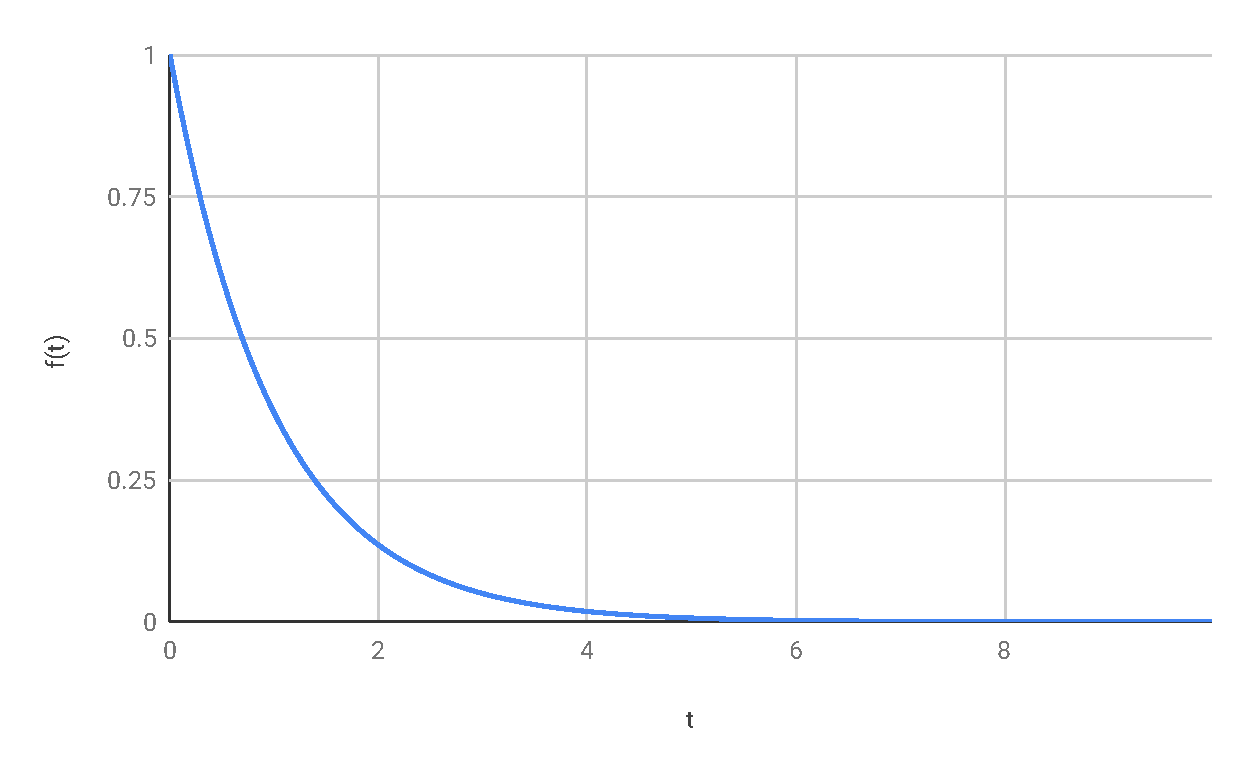
\includegraphics[scale=0.74]{image/05-RC-RL/f.pdf}
    \caption{Function $f(t)$}
    \label{figure.05.f}
\end{figure}
%%%%%%%%%%%%%%%%%%%%%%%%%%%%%%%%%%%%%%%%%%%%%%%%%%%%%%%%%%%%%%%%%%%%%%%%%%%%%%%%
\begin{figure}[ht]
    \centering
    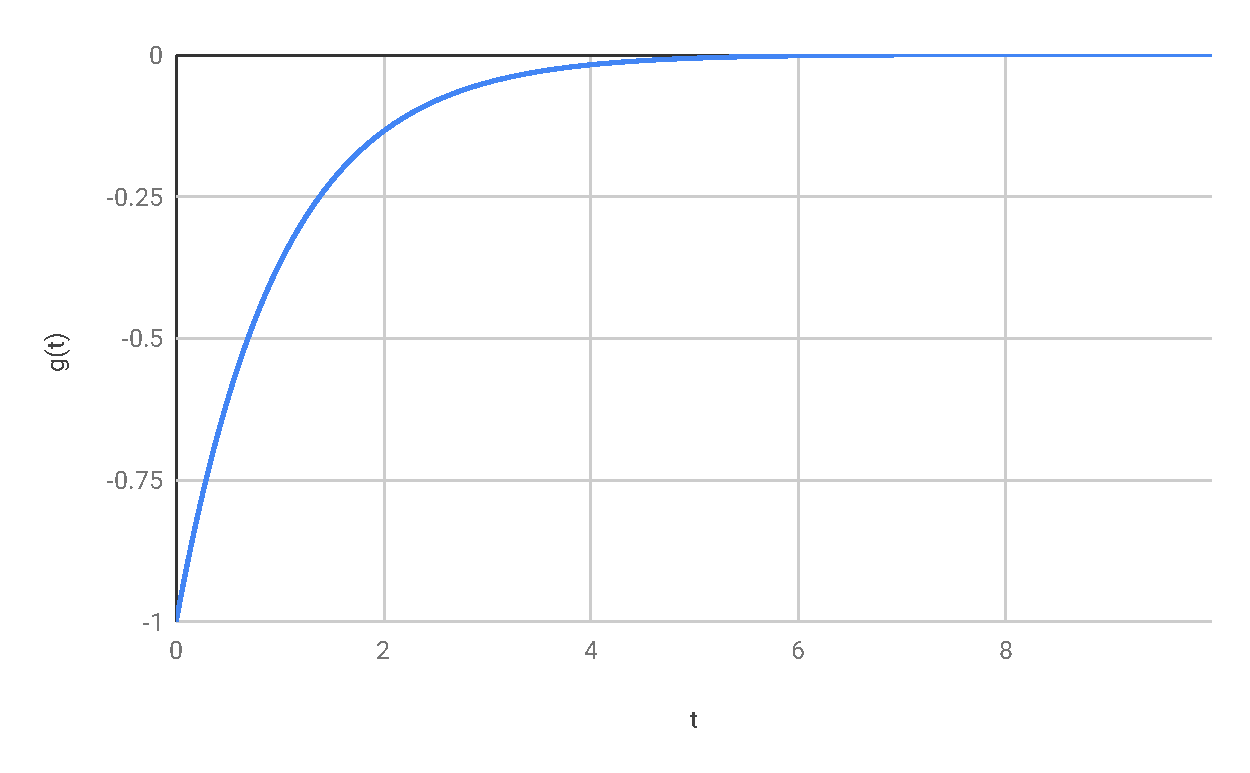
\includegraphics[scale=0.74]{image/05-RC-RL/g.pdf}
    \caption{Function $g(t)$}
    \label{figure.05.g}
\end{figure}
%%%%%%%%%%%%%%%%%%%%%%%%%%%%%%%%%%%%%%%%%%%%%%%%%%%%%%%%%%%%%%%%%%%%%%%%%%%%%%%%
\begin{figure}[ht]
    \centering
    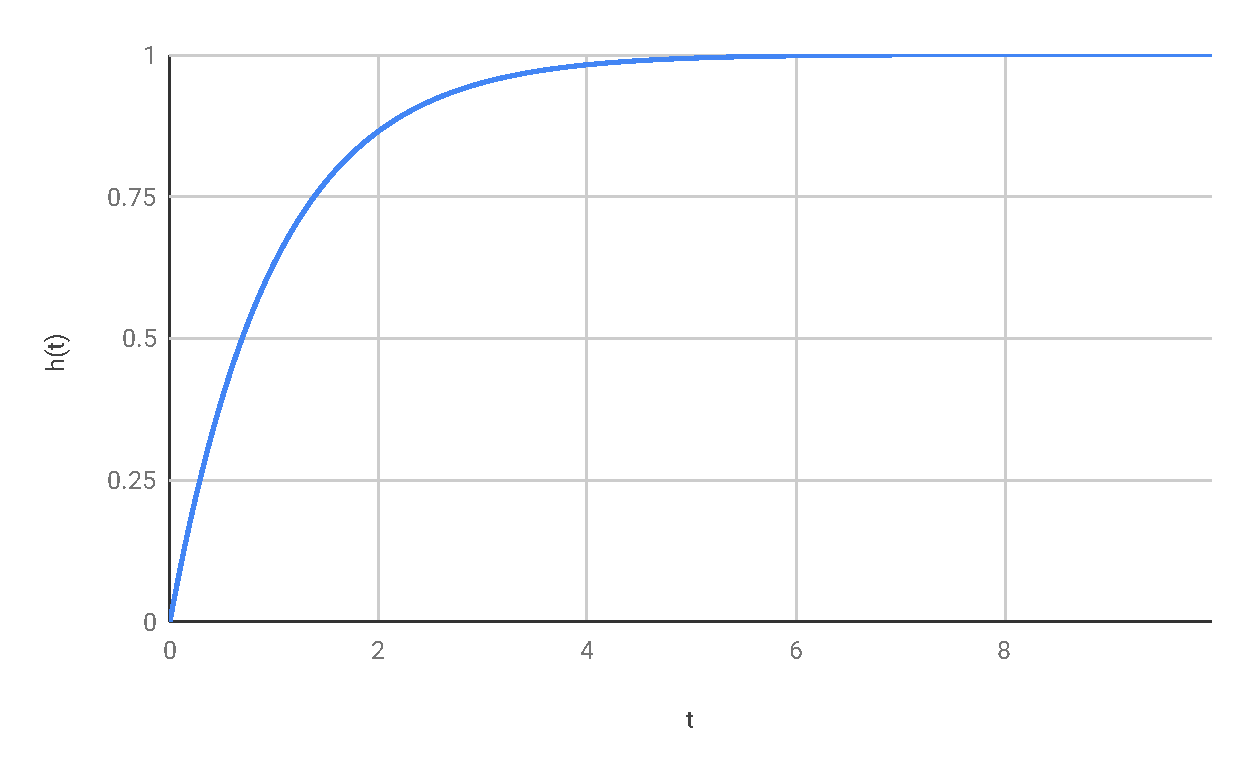
\includegraphics[scale=0.74]{image/05-RC-RL/h.pdf}
    \caption{Function $h(t)$}
    \label{figure.05.h}
\end{figure}
%%%%%%%%%%%%%%%%%%%%%%%%%%%%%%%%%%%%%%%%%%%%%%%%%%%%%%%%%%%%%%%%%%%%%%%%%%%%%%%%
\begin{figure}[ht]
    \centering
    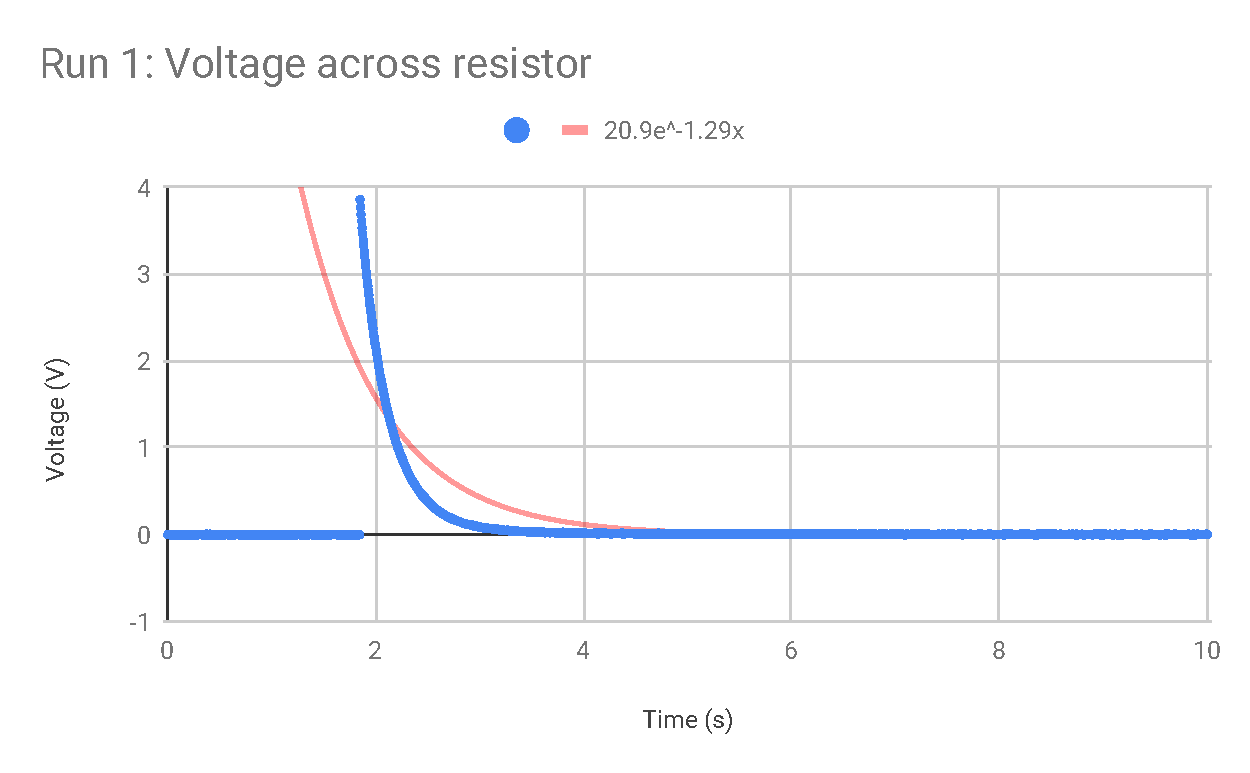
\includegraphics[scale=0.74]{image/05-RC-RL/run-1-vR-full.pdf}
    \caption{Run 1: $V_{R}(t)$}
    \label{figure.05.run.1.vR.full}
\end{figure}
%%%%%%%%%%%%%%%%%%%%%%%%%%%%%%%%%%%%%%%%%%%%%%%%%%%%%%%%%%%%%%%%%%%%%%%%%%%%%%%%
\begin{figure}[ht]
    \centering
    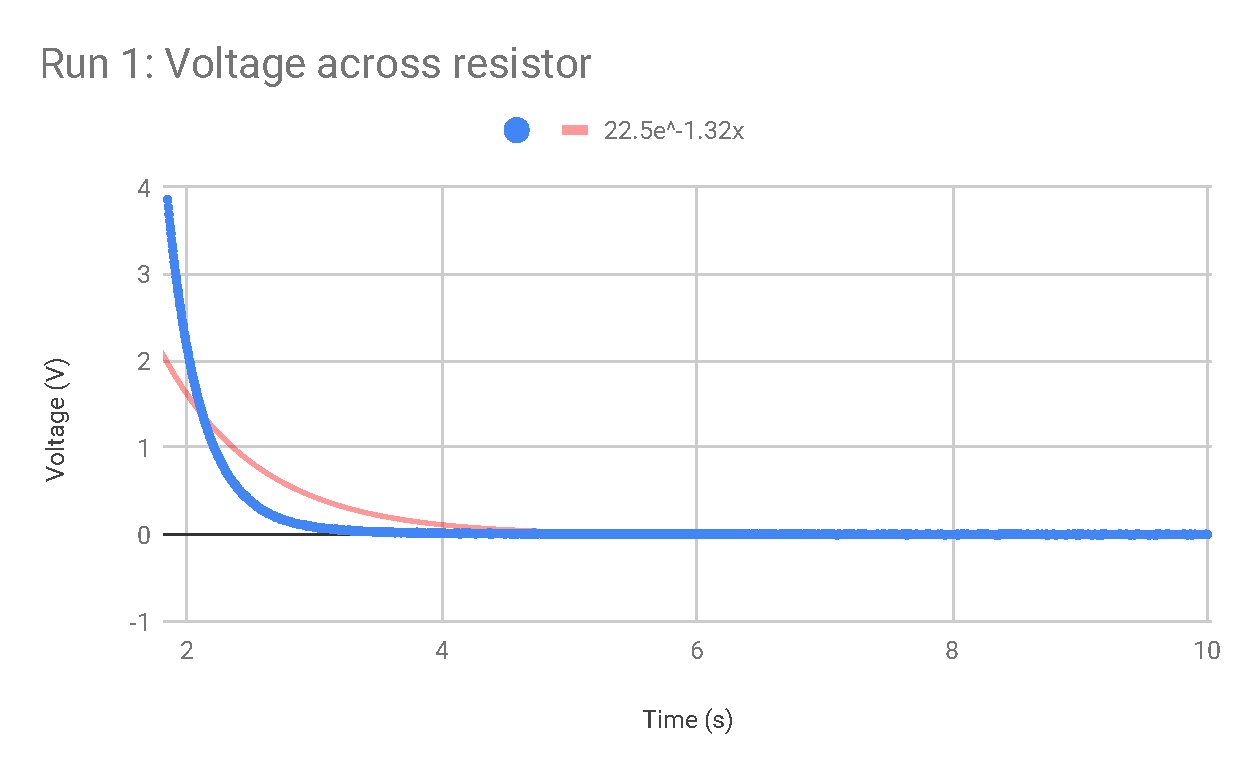
\includegraphics[scale=0.74]{image/05-RC-RL/run-1-vR-truncated.pdf}
    \caption{Run 1: $V_{R}(t)$}
    \label{figure.05.run.1.vR.truncated}
\end{figure}
%%%%%%%%%%%%%%%%%%%%%%%%%%%%%%%%%%%%%%%%%%%%%%%%%%%%%%%%%%%%%%%%%%%%%%%%%%%%%%%%
\begin{figure}[ht]
    \centering
    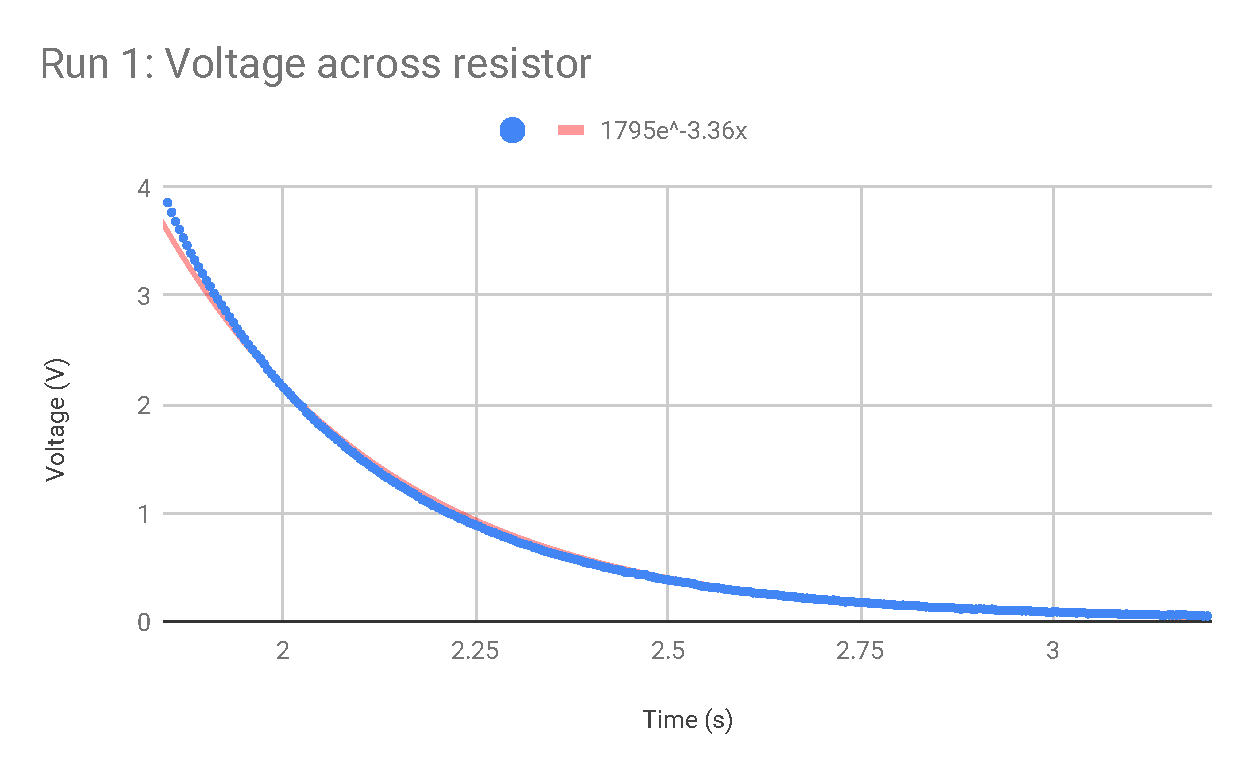
\includegraphics[scale=0.74]{image/05-RC-RL/run-1-vR-no-tail.pdf}
    \caption{Run 1: $V_{R}(t)$}
    \label{figure.05.run.1.vR.no.tail}
\end{figure}
%%%%%%%%%%%%%%%%%%%%%%%%%%%%%%%%%%%%%%%%%%%%%%%%%%%%%%%%%%%%%%%%%%%%%%%%%%%%%%%%
\begin{figure}[ht]
    \centering
    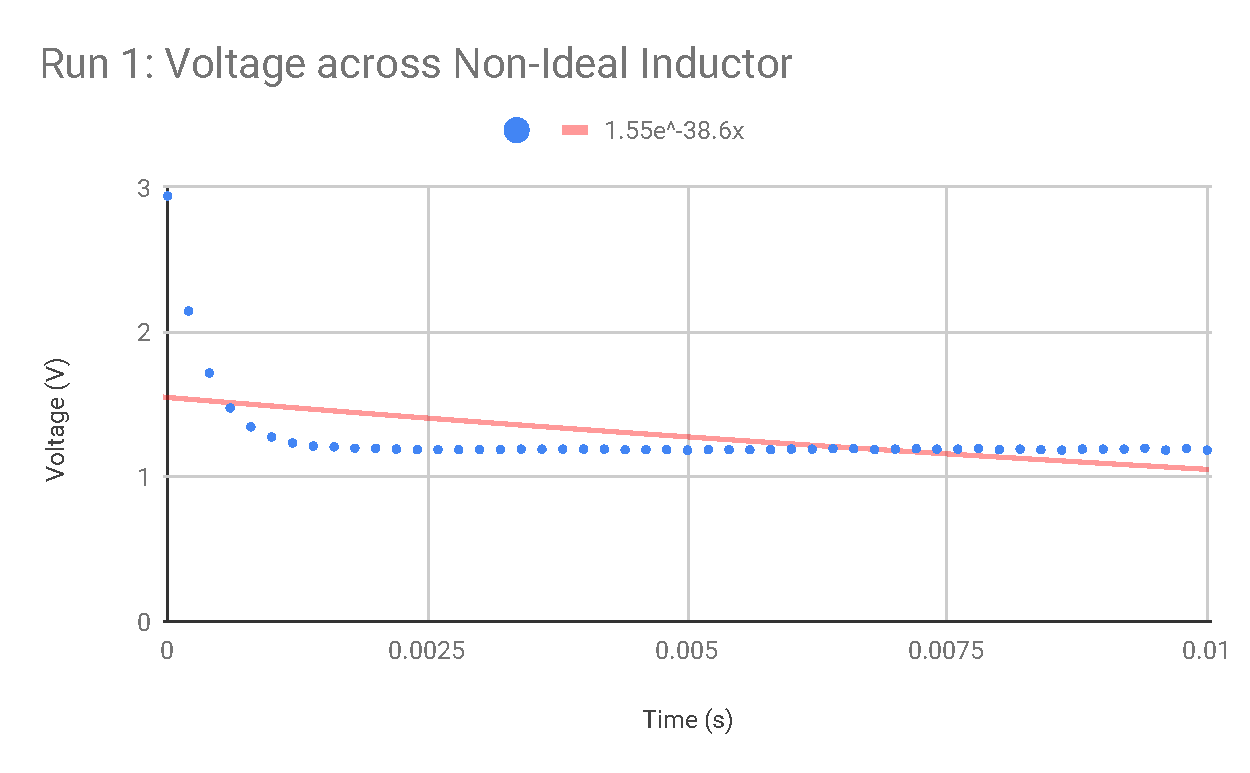
\includegraphics[scale=0.74]{image/05-RC-RL/vL-non-ideal-full.pdf}
    \caption{Run 1: $V_{r}(t) + V_{L}(t)$}
    \label{figure.05.vL.nonideal.full}
\end{figure}
%%%%%%%%%%%%%%%%%%%%%%%%%%%%%%%%%%%%%%%%%%%%%%%%%%%%%%%%%%%%%%%%%%%%%%%%%%%%%%%%
\begin{figure}[ht]
    \centering
    \includegraphics[scale=0.74]{image/05-RC-RL/vL-full.pdf}
    \caption{Run 1: $V_{L}(t)$}
    \label{figure.05.vL.full}
\end{figure}
%%%%%%%%%%%%%%%%%%%%%%%%%%%%%%%%%%%%%%%%%%%%%%%%%%%%%%%%%%%%%%%%%%%%%%%%%%%%%%%%
\begin{figure}[ht]
    \centering
    \includegraphics[scale=0.74]{image/05-RC-RL/run-1-vL.pdf}
    \caption{Run 1: $V_{L}(t)$}
    \label{figure.05.run.1.vL}
\end{figure}
% Copyright 2018-2020 Melvin Eloy Irizarry-Gelpí
\setcounter{chapter}{5}
\chapter{RLC Circuits}
%
In this experiment you will study circuits with resistors, inductors, and capacitors interacting with a source of alternating currents.
%
\section{Preliminary}
%
In a previous experiment, you studied RC and RL circuits with a \textbf{battery} (actually, a few batteries connected in series) as the source of current. Batteries provide \textbf{DC} or \textbf{direct currents}, meaning that over time the current does not change direction. Strictly speaking the previous circuits were DC circuits.

When the current switches direction over time, you have an \textbf{AC} or \textbf{alternating current}. A circuit with an AC source is called an \textbf{AC circuit}. An important parameter that describes how often an AC switches direction is $f$, the \textbf{frequency of oscillation}. Recall that frequency is a quantity measured in \textbf{hertz} (Hz). One hertz is equivalent to one full oscillation per second:
\begin{equation}
	1 \ \text{Hz} = 1 \ \text{oscillation/s}
\end{equation}
For an AC with a frequency of 1 Hz, this means that it takes 1 second for the current to do a full oscillation. Note that a full current oscillation involves two switches of current direction: the first switch changes the original direction and the second switch returns it to where it was originally. Another useful quantity is $T$, the \textbf{period of oscillation}. The period $T$ is related to the frequency $f$ via
\begin{equation} \label{eq.06.period}
	T = \frac{1}{f}
\end{equation}
Sometimes it will be useful to use frequency and sometimes it will be useful to use period.

A quick reminder that electrical \textbf{resistance} is measured in units of ohms;
\begin{equation}
	1 \ \text{ohm} = 1 \ \text{V/A}
\end{equation}
\textbf{capacitance} is measured in units of farads;
\begin{equation}
	1 \ \text{farad} = 1 \ \text{C/V} = 1 \ \text{s/ohm}
\end{equation}
and \textbf{inductance} is measured in units of henrys;
\begin{equation}
	1 \ \text{henry} = 1 \ \text{V{ }\textperiodcentered{ }s/A} = 1 \ \text{ohm{ }\textperiodcentered{ }s}
\end{equation}
%
\subsection{Reactance}
%
Resistors, capacitors and inductors behave differently in an AC circuit. Each of these components display an opposition to the change in electric current that is called \textbf{reactance}. The mathematical symbol for reactance is $X$. There is \textbf{resistive} reactance $X_{R}$, \textbf{capacitive} reactance $X_{C}$, and \textbf{inductive} reactance $X_{L}$. Each reactance quantity is measured in units of ohms (same as resistance).
%
\subsubsection{Resistive Reactance}
%
The reactance associated to a resistor is called resistive reactance. For all practical purposes, the \textbf{resistive reactance} $X_{R}$ of a given resistor is equal to the resistance $R$:
\begin{equation} \label{eq.06.reactance.R}
	X_{R} = R
\end{equation}
Note that $X_{R}$ only depends on the properties of the resistor and not on the frequency of the AC source. That is, it does not matter how often the current switches direction, the resistive reactance is the same.
%
\subsubsection{Capacitive Reactance}
%
The reactance associated to a capacitor is called capacitive reactance. The \textbf{capacitive reactance} $X_{C}$ of a given capacitor is given by
\begin{equation} \label{eq.06.reactance.C}
	X_{C} = \frac{1}{2 \pi f C} = \frac{T}{2 \pi C}
\end{equation}
Here $f$ is the frequency of oscillation of the AC source, $T$ is the period of oscillation of the AC source, and $C$ is the amount of capacitance in the capacitor. Note that $X_{C}$ is directly proportional to the period, or, equivalently, inversely proportional to the frequency. That is, if you increase the frequency of the AC source, then the reactance should decrease.
%
\subsubsection{Inductive Reactance}
%
The reactance associated to an inductor is called inductive reactance. The \textbf{inductive reactance} $X_{L}$ of a given inductor is defined as
\begin{equation} \label{eq.06.reactance.L}
	X_{L} = 2 \pi f L = \frac{2 \pi L}{T}
\end{equation}
Here $f$ is the frequency of oscillation of the AC source, $T$ is the period of oscillation of the AC source, and $L$ is the amount of inductance in the inductor. Note that $X_{L}$ is directly proportional to the frequency, or, equivalently, inversely proportional to the period. That is, if you increase the frequency of the AC source, then the reactance should increase.
%
\subsection{Impedance}
%
Reactance is associated with an individual component in a circuit. To describe the \textbf{entire circuit}, you use the \textbf{impedance} $Z$. Just like reactance and resistance, impedance is also measured in units of ohms. The exact definition of impedance depends on what the components in a circuit are. You are going to need the impedance for an RL and RLC circuit.
%
\subsubsection{RL AC Circuit}
%
An \textbf{RL AC circuit} consist of an \textbf{AC source} connected to a \textbf{resistor} and an \textbf{ideal inductor} in series. Thus there is some amount of resistive and inductive reactance. The RL impedance $Z$ takes these two contributions into account:
\begin{equation} \label{eq.06.impedance.RL}
	Z = \sqrt{X_{R}^{2} + X_{L}^{2}} = \sqrt{R^{2} + 4 \pi^{2} f^{2} L^{2}}
\end{equation}
You can think of $Z$ as the hypotenuse of a right triangle with the reactances $X_{R}$ and $X_{L}$ as sides. The squared impedance takes the form
\begin{equation} \label{eq.06.impedance.squared}
	Z^{2} = R^{2} + 4\pi^{2} f^{2} L^{2}
\end{equation}
Note that in this form, the relation between squared impedance and squared frequency lends itself for a linear fit: the intercept is the squared resistance, and the slope is proportional to the squared inductance.

An ideal inductor has negligible electrical resistance. In practice you work with \textbf{non-ideal inductors}, with a non-negligible amount of electrical resistance $r$. This can be taken into account as follows:
\begin{equation}
	Z^{2} = (R + r)^{2} + 4 \pi^{2} f^{2} L^{2}
\end{equation}
That is, the resistance from the inductor affects the value of the intercept of the linear fit.
%
\subsubsection{RLC AC Circuit}
%
An \textbf{RLC AC circuit} consist of an \textbf{AC source} connected to a \textbf{resistor}, a \textbf{capacitor}, and an \textbf{ideal inductor} in series. Now there is some amount of resistive, capacitive, and inductive reactance. The RLC impedance $Z$ now takes these three contributions into account:
\begin{equation} \label{eq.06.eq.06.impedance.RLC}
	Z = \sqrt{X_{R}^{2} + X_{L}^{2} - X_{C}^{2}} = \sqrt{R^{2} + 4 \pi^{2} f^{2} L^{2} - \frac{1}{4 \pi^{2} f^{2} C^{2}}}
\end{equation}
Something special happens when $X_{L} = X_{C}$:
\begin{align} \label{eq.06.resonant.frequency}
	X_{L}(f_{\text{LC}}) = X_{C}(f_{\text{LC}}) && \Longrightarrow && 2\pi f_{\text{LC}} L = \frac{1}{2\pi f_{\text{LC}} C} && \Longrightarrow && f_{\text{LC}} = \frac{1}{2 \pi \sqrt{LC}}
\end{align}
That is, when the frequency takes the special value $f_{\text{LC}}$ (that depends on the amount of inductance and capacitance), the impedance is given entirely by the amount of resistance. This situation is called \textbf{resonance} and $f_{\text{LC}}$ is known as the \textbf{resonant frequency}. When the values of the capacitance and inductance in the circuit conspire to achieve the resonant frequency, the impedance reduces to the resistance:
\begin{equation}
	Z = R
\end{equation}
This is the minimum value possible of impedance.
%
\section{Experiment}
%
There are four experiments:
\begin{enumerate}
	\item Capacitor in AC circuit
	\item RL AC circuit
	\item RLC AC circuit without the core
	\item RLC AC circuit with the core
\end{enumerate}
In the first two experiments you measure the voltage and current as the frequency of the AC is changed. In the last two experiments, you see the effects of the resonance state.
%
\subsection{Part 1: Capacitor AC Circuit}
%
The circuit has \textbf{one capacitor} (10\textsuperscript{\textminus 5} F) connected to an AC source whose frequency you can adjust. You measured voltage and current over time. For each measurement you change the frequency of the AC source. The range of frequencies is from 100 Hz to 1000 Hz. Table \ref{table.capacitor.student} has the frequency values used for each run.

Note that the voltage measured here is the \textbf{voltage across the capacitor}.
%
\subsection{Part 2: RL AC Circuit}
%
The circuit has \textbf{one resistor} (10 ohm) and \textbf{one non-ideal inductor} (0.005 H and 4.20 ohm) connected in series to an AC source whose frequency you can adjust. You measured voltage and current over time. For each measurement you change the frequency of the AC source. The range of frequencies is from 100 Hz to 1000 Hz. Table \ref{table.RL.student} has the frequency values used for each run.

Note that the voltage measured here is the \textbf{voltage across the resistor and inductor in series}. That is, between the input terminal of the resistor, and the output terminal of the inductor.
%
\subsection{Part 3: RLC AC Circuit (without core)}
%
The circuit has \textbf{one resistor} (in the form of a light bulb, with unknown resistance), \textbf{one capacitor} (10\textsuperscript{\textminus 5} F), and \textbf{one non-ideal inductor} (0.005 H and 4.20 ohm; without core) connected in series to an AC source whose frequency you can adjust. You measured current over time. For each measurement you change the frequency of the AC source. The range of frequencies is from 100 Hz to 1300 Hz. Table \ref{table.RLC.student} has the frequency values used for each run.
%
\subsection{Part 4: RLC AC Circuit (with core)}
%
The circuit has \textbf{one resistor} (in the form of a light bulb, with unknown resistance), \textbf{one capacitor} (10\textsuperscript{\textminus 5} F), and \textbf{one non-ideal inductor} (0.0213 H and 4.20 ohm; with core) connected in series to an AC source whose frequency you can adjust. You measured current over time. For each measurement you change the frequency of the AC source. The range of frequencies is from 100 Hz to 550 Hz. Table \ref{table.RLCcore.student} has the frequency values used for each run.
%
\section{Analysis}
%
Here is what to do for each part.
%
\subsection{Part 1: Capacitor AC Circuit}
%
The impedance of a circuit with a single capacitor is just the capacitive reactance:
\begin{equation}
	Z = X_{C} = \left(\frac{1}{2 \pi C}\right) \frac{1}{f} = \left(\frac{1}{2 \pi C}\right) T
\end{equation}
In this part you would like to check that the inductance is inversely proportional to the frequency of the AC source, or equivalently, directly proportional to the period of the AC source. You know the values of the frequencies used (and thus of the periods used), so you just need to find the experimental values of $Z$. To find this, you use the voltage and current data. For each run, you find the maximum voltage $V_{\text{max}}$ and the maximum current in $I_{\text{max}}$. Then, the impedance is given by the ratio
\begin{equation}
	Z = \frac{V_{\text{max}}}{I_{\text{max}}}
\end{equation}
Once you have the impedance, you can check that the chart of impedance versus frequency is not linear, but the chart of impedance versus period is linear. You can then add a linear fit. As stated by (\ref{eq.06.reactance.C}), the slope is related to the amount of capacitance:
\begin{equation}
	\text{slope} = \frac{1}{2 \pi C}
\end{equation}
You can calculate the expected slope, the observed slope (use the \texttt{SLOPE}) function, and then calculate the percent difference:
\begin{equation}
	\text{Percent Difference} = 100 \times \left( \frac{\text{observed } - \text{ expected}}{\text{expected}} \right)
\end{equation}
%
\subsection{Part 2: RL AC Circuit}
%
Since an RL AC circuit is used in this part, you can check the relationship between impedance $Z$ and frequency (that is, you are not measuring the reactance of individual components). The impedance is found in the same way as before:
\begin{equation}
	Z = \frac{V_{\text{max}}}{I_{\text{max}}}
\end{equation}
You can chart impedance versus frequency and the shape is almost linear. But there is no linear relationship between these two quantities! Looking at (\ref{eq.06.impedance.squared}), the expected linear relationship is between $Z^{2}$ and $f^{2}$. Make a second chart with these quantities and add a best-fit line. Compare the slope and intercept of the best-fit line to the expected values in (\ref{eq.06.impedance.squared}). The slope should be related to the inductance, and the intercept should be related to the \textbf{total amount of resistance} in the circuit. Recall that the inductor has some inherent amount of resistance, as was found in Laboratory 5:
\begin{equation}
	r = 4.20 \ \text{ohm}
\end{equation}
Adding this to the 10 ohm from the resistor, the total resistance is
\begin{equation}
	R_{\text{eq}} = R + r = 14.20 \ \text{ohm}
\end{equation}
The expected slope is
\begin{equation}
	\text{slope} = 4 \pi^{2} L^{2}
\end{equation}
and the expected intercept is
\begin{equation}
	\text{intercept} = (R + r)^{2}
\end{equation}
Again, you can also find the percent difference to judge the quality of your results.
%
\subsection{Part 3: RLC AC Circuit (without core)}
%
For the RLC circuit, you can see what happens to the current in the circuit as the frequency of the AC source  approaches the value of the resonant frequency. To do this, find the maximum current for each frequency run and then make a chart of $I_{\text{max}}$ versus frequency. There should be a peak. The peak corresponds to the resonant frequency. That is, at the resonant frequency, the current in the circuit oscillates with the largest amplitude.

The expected resonant frequency is given by (\ref{eq.06.resonant.frequency}), with the inductance equal to 0.005 H.
%
\subsection{Part 4: RLC AC Circuit (with core)}
%
In Laboratory 5 you found that when the core was used, the inductance is larger than what is written on the label. Indeed, you should have found a value close to 0.0213 H. This makes the resonant frequency smaller. You can repeat the steps as in Part 3 and confirm that the current now has a peak in a lower frequency.
%
\section{My Data}
%
My results for Part 1 are in Table \ref{table.results.C}. As you can see from Figure \ref{figure.06.part.1.f}, for this circuit, the impedance is not directly proportional to the frequency. Indeed, as you can see from Figure \ref{figure.06.part.1.T}, the impedance is directly proportional to the period of oscillation. The result is that as the frequency is increased, the impedance decreases, and thus the amount of current allowed increases.

My results for Part 2 are in Table \ref{table.results.RL}. Figure \ref{figure.06.part.2.f} appears to indicate that the impedance is directly proportional to the amount of frequency. However, the best fit is off for some values. Looking at the squared impedance versus the squared frequency in Figure \ref{figure.06.part.2.f2} shows that the linear relation is stronger between those two quantities. Opposite to what happens in Part 1, when the frequency is increased, the impedance also increases, and thus the amount of current allowed decreases.

My results for Part 3 are in Table \ref{table.results.RLC}. As you can see from Figure \ref{figure.06.part.3.f}, the current is largest in a certain region consistent with the theoretical expectation. Note that when the current is largest, the impedance is smallest.

My results for Part 4 are in Table \ref{table.results.RLCcore}. When the core is used, the inductance becomes larger. This should have the effect of making the resonant frequency smaller. As Figure \ref{figure.06.part.4.f} shows, this is indeed the case.
%
\section{Your Data}
%
Your data for Parts 1, 2, 3, and 4 is structured in the same way as Tables \ref{table.capacitor.student}, \ref{table.RL.student}, \ref{table.RLC.student}, and \ref{table.RLCcore.student}.
%
\pagebreak
\section{Your Lab Report}
%
Your laboratory report should include the following:
\begin{itemize}
	\item A table like Table \ref{table.results.C} with your results for part 1.
	\item A chart like Figure \ref{figure.06.part.1.T} with impedance in the vertical axis, and period in the horizontal axis for the data in part 1. Include the best fit line and display the equation.
	\item A table like Table \ref{table.results.RL} with your results for part 2.
	\item A chart like Figure \ref{figure.06.part.2.f2} with squared impedance in the vertical axis, and squared frequency in the horizontal axis for the data in part 2. Include the best fit line and display the equation.
	\item A chart like Figure \ref{figure.06.part.3.f} with maximum current in the vertical axis, and frequency in the horizontal axis for the data in part 3. Confirm that the maximum current corresponds occurs near frequencies that are close to the expected resonant frequency.
	\item A chart like Figure \ref{figure.06.part.4.f} with maximum current in the vertical axis, and frequency in the horizontal axis for the data in part 4. Confirm that the maximum current corresponds occurs near frequencies that are close to the expected resonant frequency.
\end{itemize}
%
\newpage
\section{Tables}
%
\begin{table}[ht]
	\begin{center}
		\begin{tabular}{l|r|r|r|r|r}
			\textbf{Run} & $f$ (Hz) & $1/f$ (s) & $V_{\text{max}}$ (V) & $I_{\text{max}}$ (A) & $V_{\text{max}}/I_{\text{max}}$ (ohm) \\
			\hline
			1 & 100 & & & & \\
			2 & 250 & & & & \\
			3 & 400 & & & & \\
			4 & 550 & & & & \\
			5 & 700 & & & & \\
			6 & 850 & & & & \\
			7 & 1000 & & & & \\
			\hline
		\end{tabular}
	\end{center}
	\caption{Capacitor AC Circuit}
	\label{table.capacitor.student}
\end{table}
%
\begin{table}[ht]
	\begin{center}
		\begin{tabular}{l|r|r|r|r|r}
			\textbf{Run} & $f$ (Hz) & $1/f$ (s) & $V_{\text{max}}$ (V) & $I_{\text{max}}$ (A) & $V_{\text{max}}/I_{\text{max}}$ (ohm) \\
			\hline
			1 & 100 & & & & \\
			2 & 250 & & & & \\
			3 & 400 & & & & \\
			4 & 550 & & & & \\
			5 & 700 & & & & \\
			6 & 850 & & & & \\
			7 & 1000 & & & & \\
			\hline
		\end{tabular}
	\end{center}
	\caption{RL AC Circuit}
	\label{table.RL.student}
\end{table}
%
\begin{table}[ht]
	\begin{center}
		\begin{tabular}{l|r|r}
			\textbf{Run} & $f$ (Hz) & $I_{\text{max}}$ (A) \\
			\hline
			1 & 100 & \\
			2 & 250 & \\
			3 & 400 & \\
			4 & 550 & \\
			5 & 700 & \\
			6 & 850 & \\
			7 & 1000 & \\
			8 & 1150 & \\
			9 & 1300 & \\
			\hline
		\end{tabular}
	\end{center}
	\caption{RLC AC Circuit without core}
	\label{table.RLC.student}
\end{table}
%
\begin{table}[ht]
	\begin{center}
		\begin{tabular}{l|r|r}
			\textbf{Run} & $f$ (Hz) & $I_{\text{max}}$ (A) \\
			\hline
			1 & 100 & \\
			2 & 250 & \\
			3 & 400 & \\
			4 & 550 & \\
			5 & 200 & \\
			6 & 300 & \\
			7 & 350 & \\
			8 & 450 & \\
			9 & 500 & \\
			\hline
		\end{tabular}
	\end{center}
	\caption{RLC AC Circuit with core}
	\label{table.RLCcore.student}
\end{table}
%
\begin{table}[ht]
	\begin{center}
		\begin{tabular}{l|r|r|r}
			\textbf{Quantity} & \textbf{Observed} & \textbf{Expected} & \textbf{P.D.} (\%) \\
			\hline
			Slope (ohm/s) & 14683.346 & 15915.494 & \textminus 7.742 \\
			\hline
		\end{tabular}
	\end{center}
	\caption{Results for capacitor AC circuit}
	\label{table.results.C}
\end{table}
%
\begin{table}[ht]
	\begin{center}
		\begin{tabular}{l|r|r|r}
			\textbf{Quantity} & \textbf{Observed} & \textbf{Expected} & \textbf{P.D.} (\%) \\
			\hline
			Slope (ohm\textsuperscript{2}/Hz\textsuperscript{2}) & 9.87{ }\texttimes{ }10\textsuperscript{\textminus 4} & 9.92{ }\texttimes{ }10\textsuperscript{\textminus 4} & 0.52 \\
			Intercept (ohm\textsuperscript{2}) & 199.778 & 201.64 & \textminus 0.924 \\
			\hline
		\end{tabular}
	\end{center}
	\caption{Results for RL AC circuit}
	\label{table.results.RL}
\end{table}
%
\begin{table}[ht]
	\begin{center}
		\begin{tabular}{l|r}
			Observed Resonant Frequency & Expected Resonant Frequency \\
			\hline
			Between 700 Hz and 800 Hz & 711.76 Hz \\
			\hline
		\end{tabular}
	\end{center}
	\caption{Results for RLC AC circuit (without core)}
	\label{table.results.RLC}
\end{table}
%
\begin{table}[ht]
	\begin{center}
		\begin{tabular}{l|r}
			Observed Resonant Frequency & Expected Resonant Frequency \\
			\hline
			Between 300 Hz and 350 Hz & 344.85 Hz \\
			\hline
		\end{tabular}
	\end{center}
	\caption{Results for RLC AC circuit (with core)}
	\label{table.results.RLCcore}
\end{table}
%
\newpage
\FloatBarrier
\section{Figures}
%
\begin{figure}[ht]
	\centering
	\includegraphics[scale=0.74]{image/06-RLC/part-1-f.pdf}
	\caption{Part 1: Period}
	\label{figure.06.part.1.f}
\end{figure}
%
\begin{figure}[ht]
	\centering
	\includegraphics[scale=0.74]{image/06-RLC/part-1-T.pdf}
	\caption{Part 1: Frequency}
	\label{figure.06.part.1.T}
\end{figure}
%
\begin{figure}[ht]
	\centering
	\includegraphics[scale=0.74]{image/06-RLC/part-2-f.pdf}
	\caption{Part 2: Frequency}
	\label{figure.06.part.2.f}
\end{figure}
%
\begin{figure}[ht]
	\centering
	\includegraphics[scale=0.74]{image/06-RLC/part-2-f2.pdf}
	\caption{Part 2: Squared Frequency}
	\label{figure.06.part.2.f2}
\end{figure}
%
\begin{figure}[ht]
	\centering
	\includegraphics[scale=0.74]{image/06-RLC/part-3.pdf}
	\caption{Part 3}
	\label{figure.06.part.3.f}
\end{figure}
%
\begin{figure}[ht]
	\centering
	\includegraphics[scale=0.74]{image/06-RLC/part-4.pdf}
	\caption{Part 4}
	\label{figure.06.part.4.f}
\end{figure}
%
%
% \part{Optics}
%
% % Copyright 2018-2020 Melvin Eloy Irizarry-Gelpí
\setcounter{chapter}{6}
\chapter{Curved Mirrors}
%
In this experiment you will learn about the properties of images produced by curved mirrors.
%
\section{Preliminary}
%
A mirror reflects light. Mirrors can be flat or curved. Flat mirrors are commonly found in bathrooms. Curved mirrors can either be concave or convex. As you will see, a concave mirror can produce a real image, in the sense that the image can be projected on a screen.

Light is emitted from an \textbf{object}. This light travels through space and then bounces of a mirror, potentially producing an \textbf{image} somewhere in space. There is a relationship between the distance between the object and the mirror, $d_{O}$, and the distance between the image and the mirror, $d_{I}$. This relationship involves a property of the mirror called the focal length $f$:
\begin{equation}
    \frac{1}{d_{O}} + \frac{1}{d_{I}} = \frac{1}{f}
\end{equation}
This is a curious relation because it involves the inverse quantities, and not the direct quantities themselves. Another way of writing this relation is as
\begin{equation}
    \frac{1}{d_{I}} = -\frac{1}{d_{O}} + \frac{1}{f}
\end{equation}
If you measure $d_{O}$ and $d_{I}$, then the chart with $1/d_{I}$ in the vertical axis and $1/d_{O}$ in the horizontal axis should have a linear shape. The slope of the line should be close to $-1$, and the value of the intercept should be close to the inverse of the focal length of the mirror used.

In practice it is easier to measure position than to measure distance. You have three things: the object, the image, and the mirror. Thus you have three positions along the track: the position $x_{O}$ of the object, the position $x_{I}$ of the image, and the position $x_{M}$ of the mirror. The distance between the object and the mirror is simply
\begin{equation}
    d_{O} = \left\vert x_{O} - x_{M} \right\vert
\end{equation}
Similarly, the distance between the image and the mirror is given by
\begin{equation}
    d_{I} = \left\vert x_{I} - x_{M} \right\vert
\end{equation}
%
\subsection{Magnification}
%
Curved mirrors produce images that look very different from the object that is emitting the light. Some differences can involve a change in \textbf{orientation}. For example, left and right can be switched, as is common with plane mirrors. Other differences can be a change in \textbf{size}. That is, the size of an image can be smaller or larger than the object. There is a quantity called magnification that is used to describe how the size of an image compares to the size of the object. Let $h_{I}$ be the height of the image, and $h_{O}$ be the height of the object. The magnification $m$ of the mirror is given by the ratio
\begin{equation}
    m = \frac{h_{I}}{h_{O}}
\end{equation}
Note that magnification has no units because it is the ratio of two lengths. There is another definition of the magnification that involves the distances from the mirror to the object and the image:
\begin{equation}
    m = \frac{d_{I}}{d_{O}}
\end{equation}
This particular definition is missing a minus sign that is traditionally used to denote a change in orientation. For practical purposes, you can ignore that minus sign.
%
\section{Experiment}
%
The experiment with the concave mirror consisted of recording the position of the mirror, the object, and the screen where the sharp image is projected. You also used a ruler to record the height of the object and the image.
%
\section{Analysis}
%
With the position of the object, mirror, and image you can calculate the distances $d_{O}$ and $d_{I}$. Then you can make a chart of $1 / d_{I}$ versus $1 / d_{O}$. The expected relation is
\begin{equation}
    \frac{1}{d_{I}} = -\frac{1}{d_{O}} + \frac{1}{f}
\end{equation}
The slope of the best fit line should be:
\begin{equation}
    \text{slope} = -1
\end{equation}
From the intercept you can find an experimental estimate of the focal length of the mirror:
\begin{equation}
    \text{focal length} = \frac{1}{\text{intercept}}
\end{equation}
The expected value for the focal length of the concave mirror used is 20 cm.

With the distances $d_{O}$ and $d_{I}$ you can calculate the magnification:
\begin{equation}
    m = \frac{d_{I}}{d_{O}}
\end{equation}
You can also calculate the magnification using the measured heights $h_{I}$ and $h_{O}$:
\begin{equation}
    m = \frac{h_{I}}{h_{O}}
\end{equation}
both of these methods should be consistent.
%
\section{My Data}
%
My data consist of ten distinct configurations. As can be seen from Figure \ref{figure.07.chart}, the expected behavior is observed between the inverse distances to the mirror. Further more, the slope and intercept agree with the expected values.

You can also see from Table \ref{table.07.magnification} that the two ways of computing the magnification of the mirror give similar results.
%
\section{Your Data}
%
You should have positions and heights for eight distinct configurations.
%
\newpage
\section{Your Lab Report}
%
Your laboratory report should include the following:
\begin{itemize}
    \item A table like Table \ref{table.07.magnification} with the magnification computed in two different ways.
    \item A chart with $d_{I}$ in the vertical axis, and $d_{O}$ in the horizontal axis.
    \item A chart with $1/d_{I}$ in the vertical axis, and $1/d_{O}$ in the horizontal axis. Include the best linear fit, and display the equation. See Figure \ref{figure.07.chart}.
    \item A table like Table \ref{table.07.results} with your results and the percent differences.
    \item Answer the following question: which method of calculating the magnification do you think is more accurate?
\end{itemize}
%
\newpage
\section{Tables}
%
\begin{table}[ht]
    \centering
    \begin{tabular}{|r|r|r|}
        \hline
        $x_{O}$ (cm) & $x_{M}$ (cm) & $x_{I}$ (cm) \\
        \hline
        10 & 120 & 96.05 \\
        10 & 112 & 87.35 \\
        10 & 104 & 79.1 \\
        10 & 96 & 70.15 \\
        10 & 88 & 61.35 \\
        10 & 80 & 52.55 \\
        10 & 72 & 43.05 \\
        10 & 64 & 32.5 \\
        10 & 56 & 21.35 \\
        60 & 90 & 36.2 \\
        \hline
    \end{tabular}
    \caption{Raw Position Data}
    \label{table.07.position}
\end{table}
%
\begin{table}[ht]
    \centering
    \begin{tabular}{|r|r|}
        \hline
        $h_{O}$ (cm) & $h_{I}$ (cm) \\
        \hline
        2 & 0.5 \\
        2 & 0.5 \\
        2 & 0.5 \\
        2 & 0.7 \\
        2 & 0.7 \\
        2 & 0.8 \\
        2 & 0.9 \\
        2 & 1.1 \\
        2 & 1.4 \\
        2 & 3.5 \\
        \hline
    \end{tabular}
    \caption{Raw Height Data}
    \label{table.07.height}
\end{table}
%
\begin{table}[ht]
    \centering
    \begin{tabular}{|r|r|}
        \hline
        $d_{O}$ (cm) & $d_{I}$ (cm) \\
        \hline
        110 & 23.95 \\
        102 & 24.65 \\
        94 & 24.9 \\
        86 & 25.85 \\
        78 & 26.65 \\
        70 & 27.45 \\
        62 & 28.95 \\
        54 & 31.5 \\
        46 & 34.65 \\
        30 & 53.8 \\
        \hline
    \end{tabular}
    \caption{Distances to the mirror}
    \label{table.07.distance}
\end{table}
%
\begin{table}[ht]
    \centering
    \begin{tabular}{|r|r|}
        \hline
        $h_{I} / h_{O}$ & $d_{I} / d_{O}$ \\
        \hline
        0.25 & 0.22 \\
        0.25 & 0.24 \\
        0.25 & 0.26 \\
        0.35 & 0.30 \\
        0.35 & 0.34 \\
        0.4 & 0.39 \\
        0.45 & 0.45 \\
        0.55 & 0.58 \\
        0.7 & 0.75 \\
        1.75 & 1.79 \\
        \hline
    \end{tabular}
    \caption{Magnification}
    \label{table.07.magnification}
\end{table}
%
\begin{table}[ht]
    \centering
    \begin{tabular}{|l|r|r|r|}
        \hline
        Name & Expected Value & Observed Value & P.D. (\%) \\
        \hline
        Slope & $-1$ & $-0.95$ & $-4.68$ \\
        Focal Length & 20 cm & 20.02 cm & $0.11$ \\
        \hline
    \end{tabular}
    \caption{Results}
    \label{table.07.results}
\end{table}
%
\newpage
\FloatBarrier
\section{Figures}
%
\begin{figure}[ht]
    \centering
    \includegraphics[scale=0.74]{image/07-mirrors/chart.pdf}
    \caption{Linear fit}
    \label{figure.07.chart}
\end{figure}
%
% % Copyright 2018-2019 Melvin Eloy Irizarry-Gelpí
\setcounter{chapter}{7}
\chapter{Thin Lenses}
%%%%%%%%%%%%%%%%%%%%%%%%%%%%%%%%%%%%%%%%%%%%%%%%%%%%%%%%%%%%%%%%%%%%%%%%%%%%%%%%
...
%%%%%%%%%%%%%%%%%%%%%%%%%%%%%%%%%%%%%%%%%%%%%%%%%%%%%%%%%%%%%%%%%%%%%%%%%%%%%%%%
\section{Preliminary}
%%%%%%%%%%%%%%%%%%%%%%%%%%%%%%%%%%%%%%%%%%%%%%%%%%%%%%%%%%%%%%%%%%%%%%%%%%%%%%%%
...
%%%%%%%%%%%%%%%%%%%%%%%%%%%%%%%%%%%%%%%%%%%%%%%%%%%%%%%%%%%%%%%%%%%%%%%%%%%%%%%%
\section{Experiment}
%%%%%%%%%%%%%%%%%%%%%%%%%%%%%%%%%%%%%%%%%%%%%%%%%%%%%%%%%%%%%%%%%%%%%%%%%%%%%%%%
...
%%%%%%%%%%%%%%%%%%%%%%%%%%%%%%%%%%%%%%%%%%%%%%%%%%%%%%%%%%%%%%%%%%%%%%%%%%%%%%%%
\section{Analysis}
%%%%%%%%%%%%%%%%%%%%%%%%%%%%%%%%%%%%%%%%%%%%%%%%%%%%%%%%%%%%%%%%%%%%%%%%%%%%%%%%
...
%%%%%%%%%%%%%%%%%%%%%%%%%%%%%%%%%%%%%%%%%%%%%%%%%%%%%%%%%%%%%%%%%%%%%%%%%%%%%%%%
\section{My Data}
%%%%%%%%%%%%%%%%%%%%%%%%%%%%%%%%%%%%%%%%%%%%%%%%%%%%%%%%%%%%%%%%%%%%%%%%%%%%%%%%
...
%%%%%%%%%%%%%%%%%%%%%%%%%%%%%%%%%%%%%%%%%%%%%%%%%%%%%%%%%%%%%%%%%%%%%%%%%%%%%%%%
\section{Your Data}
%%%%%%%%%%%%%%%%%%%%%%%%%%%%%%%%%%%%%%%%%%%%%%%%%%%%%%%%%%%%%%%%%%%%%%%%%%%%%%%%
...
%%%%%%%%%%%%%%%%%%%%%%%%%%%%%%%%%%%%%%%%%%%%%%%%%%%%%%%%%%%%%%%%%%%%%%%%%%%%%%%%
\section{Your Lab Report}
%%%%%%%%%%%%%%%%%%%%%%%%%%%%%%%%%%%%%%%%%%%%%%%%%%%%%%%%%%%%%%%%%%%%%%%%%%%%%%%%
...
% % Copyright 2018-2019 Melvin Eloy Irizarry-Gelpí
\setcounter{chapter}{8}
\chapter{Aperture and Depth of Field}
%%%%%%%%%%%%%%%%%%%%%%%%%%%%%%%%%%%%%%%%%%%%%%%%%%%%%%%%%%%%%%%%%%%%%%%%%%%%%%%%
In this experiment you will learn about the effect of aperture on depth of field.
%%%%%%%%%%%%%%%%%%%%%%%%%%%%%%%%%%%%%%%%%%%%%%%%%%%%%%%%%%%%%%%%%%%%%%%%%%%%%%%%
\section{Preliminary}
%%%%%%%%%%%%%%%%%%%%%%%%%%%%%%%%%%%%%%%%%%%%%%%%%%%%%%%%%%%%%%%%%%%%%%%%%%%%%%%%
Given an object in position $x_{O}$ and a convex lens in position $x_{L}$ with focal length $f$, a perfectly sharp image will form in position $x_{I}$. As found in the previous experiment, the three positions and the focal length are related via:
\begin{equation}
    \frac{1}{d_{O}} + \frac{1}{d_{I}} = \frac{1}{\vert x_{O} - x_{L} \vert} + \frac{1}{\vert x_{I} - x_{L} \vert} = \frac{1}{f}
\end{equation}
Indeed, there is some wiggle room around the position of the perfectly sharp image where the image is still relatively in focus. The \textbf{depth of field} is defined as the range of positions where a real image from a convex lens is reasonably focused, according to some specific criterion. In this experiment you will use the following criterion: can two distinct lines in an image be distinguished?
%%%%%%%%%%%%%%%%%%%%%%%%%%%%%%%%%%%%%%%%%%%%%%%%%%%%%%%%%%%%%%%%%%%%%%%%%%%%%%%%
\subsection{Near Limit}
%%%%%%%%%%%%%%%%%%%%%%%%%%%%%%%%%%%%%%%%%%%%%%%%%%%%%%%%%%%%%%%%%%%%%%%%%%%%%%%%
The \textbf{near limit} $D_{N}$ is the distance between the object and the lens when the lens is as \textbf{near} to the object as possible and features in the image are close to being blurred.
%%%%%%%%%%%%%%%%%%%%%%%%%%%%%%%%%%%%%%%%%%%%%%%%%%%%%%%%%%%%%%%%%%%%%%%%%%%%%%%%
\subsection{Far Limit}
%%%%%%%%%%%%%%%%%%%%%%%%%%%%%%%%%%%%%%%%%%%%%%%%%%%%%%%%%%%%%%%%%%%%%%%%%%%%%%%%
The \textbf{far limit} $D_{F}$ is the distance between the object and the lens when the lens is as \textbf{far} from the object as possible and features in the image are close to being blurred.
%%%%%%%%%%%%%%%%%%%%%%%%%%%%%%%%%%%%%%%%%%%%%%%%%%%%%%%%%%%%%%%%%%%%%%%%%%%%%%%%
\subsection{Depth of Field}
%%%%%%%%%%%%%%%%%%%%%%%%%%%%%%%%%%%%%%%%%%%%%%%%%%%%%%%%%%%%%%%%%%%%%%%%%%%%%%%%
The near and far limits tell you how close or how far away can and object be while still being relatively in focus. The size of this region in space is known as the depth of field. Given the values of the near limit $D_{N}$ and the far limit $D_{F}$, you can find the depth of field via:
\begin{equation}
    \text{depth of field} = D_{F} - D_{N}
    \label{eq.09.dof}
\end{equation}
It turns out that the value of the near limit, the far limit, and the depth of field can all be changed by using different apertures. An \textbf{aperture} is a space opening between the lens and the image. For example, the pupil of the eye serves as the aperture for the eye. As the pupil changes size, the eye's depth of field changes: near objects can come to sharp focus or vice versa.
%%%%%%%%%%%%%%%%%%%%%%%%%%%%%%%%%%%%%%%%%%%%%%%%%%%%%%%%%%%%%%%%%%%%%%%%%%%%%%%%
\subsection{f-Numbers}
%%%%%%%%%%%%%%%%%%%%%%%%%%%%%%%%%%%%%%%%%%%%%%%%%%%%%%%%%%%%%%%%%%%%%%%%%%%%%%%%
The f-number $N_{f}$ is a value used to describe an aperture of a lens:
\begin{equation}
    N_{f} = \frac{f}{d}
\end{equation}
Here $f$ is the focal length of the lens, and $d$ is the diameter of the aperture.

In photography, it is common to find combinations of lens ($f$) and aperture ($d$) that produce certain values of f-number. More information about f-numbers can be found in Wikipedia:
\begin{center}
    \url{https://en.wikipedia.org/wiki/F-number}
\end{center}
In this experiment you will have five different apertures available. Each aperture is labeled with a number from 1 to 5, and has a different diameter. Hence, each aperture will have a different f-number. You can check that the following ratios are fixed:
\begin{equation}
    \frac{N_{4}}{N_{5}} = \frac{N_{3}}{N_{4}} = \frac{N_{2}}{N_{3}} = \frac{N_{1}}{N_{2}} = \sqrt{2} \approx 1.4142\ldots
\end{equation}
Here $N_{5}$ is the f-number for the aperture labeled with 5, and so on.
%%%%%%%%%%%%%%%%%%%%%%%%%%%%%%%%%%%%%%%%%%%%%%%%%%%%%%%%%%%%%%%%%%%%%%%%%%%%%%%%
\section{Experiment}
%%%%%%%%%%%%%%%%%%%%%%%%%%%%%%%%%%%%%%%%%%%%%%%%%%%%%%%%%%%%%%%%%%%%%%%%%%%%%%%%
You used the 20 cm double convex lens and five different apertures. For each aperture you measured the diameter. You also found the near and far limits for each aperture.
%%%%%%%%%%%%%%%%%%%%%%%%%%%%%%%%%%%%%%%%%%%%%%%%%%%%%%%%%%%%%%%%%%%%%%%%%%%%%%%%
\section{Analysis}
%%%%%%%%%%%%%%%%%%%%%%%%%%%%%%%%%%%%%%%%%%%%%%%%%%%%%%%%%%%%%%%%%%%%%%%%%%%%%%%%
Instead of measuring the near and far limits directly, you measured the positions of the object and lens. The near and far limits can be found in the same way that the object distance is calculated:
\begin{equation}
    \vert x_{O} - x_{L} \vert
\end{equation}
Once the near and far limits are obtained, you can find the depth of field using Equation \ref{eq.09.dof}.
%%%%%%%%%%%%%%%%%%%%%%%%%%%%%%%%%%%%%%%%%%%%%%%%%%%%%%%%%%%%%%%%%%%%%%%%%%%%%%%%
\section{Your Report}
%%%%%%%%%%%%%%%%%%%%%%%%%%%%%%%%%%%%%%%%%%%%%%%%%%%%%%%%%%%%%%%%%%%%%%%%%%%%%%%%
Your report should include the following:
\begin{itemize}
    \item A table like Table \ref{table.09.fnumbers} with the diameter measurements and the values of the f-Number determined.
    \item A table like Table \ref{table.09.ratios} with the ratios of consecutive f-numbers. Include the percent difference found by comparing each ratio with the expected value $\sqrt{2} \approx 1.4142$.
    \item A table like Table \ref{table.09.results} with the rest of the results: include the near and far limits, and also the depth of field for each aperture.
    \item A scatter chart with depth of field in the vertical axis, and aperture diameter in the horizontal axis. Make sure you label each axis.
\end{itemize}
You should answer the following questions:
\begin{enumerate}
    \item Which aperture has the largest near limit?
    \item Which aperture has the largest far limit?
    \item Which aperture has the largest depth of field?
    \item Looking at your chart of depth of field versus diameter, what happens to the values of depth of field as you make the diameter smaller?
\end{enumerate}
%%%%%%%%%%%%%%%%%%%%%%%%%%%%%%%%%%%%%%%%%%%%%%%%%%%%%%%%%%%%%%%%%%%%%%%%%%%%%%%%
\newpage
\section{Tables}
%%%%%%%%%%%%%%%%%%%%%%%%%%%%%%%%%%%%%%%%%%%%%%%%%%%%%%%%%%%%%%%%%%%%%%%%%%%%%%%%
\begin{table}[ht]
    \begin{center}
        \begin{tabular}{|l|r|r|}
            \hline
            Aperture Label & Diameter (cm) & f-Number \\
            \hline
            5 & & \\
            4 & & \\
            3 & & \\
            2 & & \\
            1 & & \\
            \hline
        \end{tabular}
    \end{center}
    \caption{f-Numbers for apertures with 20 cm double convex lens}
    \label{table.09.fnumbers}
\end{table}
%%%%%%%%%%%%%%%%%%%%%%%%%%%%%%%%%%%%%%%%%%%%%%%%%%%%%%%%%%%%%%%%%%%%%%%%%%%%%%%%
\begin{table}[ht]
    \begin{center}
        \begin{tabular}{|l|r|r|r|}
            \hline
            Ratio & Observed Value & Expected Value & P.D. (\%) \\
            \hline
            $N_{4} / N_{5}$ & & 1.4142 & \\
            $N_{3} / N_{4}$ & & 1.4142 & \\
            $N_{2} / N_{3}$ & & 1.4142 & \\
            $N_{1} / N_{2}$ & & 1.4142 & \\
            \hline
        \end{tabular}
    \end{center}
    \caption{Ratios of consecutive f-numbers}
    \label{table.09.ratios}
\end{table}
%%%%%%%%%%%%%%%%%%%%%%%%%%%%%%%%%%%%%%%%%%%%%%%%%%%%%%%%%%%%%%%%%%%%%%%%%%%%%%%%
\begin{table}[ht]
    \begin{center}
        \begin{tabular}{|l|r|r|r|}
            \hline
            Aperture Label & $D_{N}$ (cm) & $D_{F}$ (cm) & $D_{F} - D_{N}$ (cm) \\
            \hline
            5 & & & \\
            4 & & & \\
            3 & & & \\
            2 & & & \\
            1 & & & \\
            \hline
        \end{tabular}
    \end{center}
    \caption{Results}
    \label{table.09.results}
\end{table}
%%%%%%%%%%%%%%%%%%%%%%%%%%%%%%%%%%%%%%%%%%%%%%%%%%%%%%%%%%%%%%%%%%%%%%%%%%%%%%%%
% % Copyright 2018-2020 Melvin Eloy Irizarry-Gelpí
\setcounter{chapter}{9}
\chapter{Interference}
%
In this experiment you will learn about interference in light from a laser due to a double slit.
%
\section{Preliminary}
%
In the previous three experiments you studied phenomena like reflection and refraction that can be explained with the \textbf{ray} model of light. Interference and diffraction are two phenomena that are easier to explain with the \textbf{wave} model of light. Both of these have to do with light passing throw an opening or openings. But unlike the apertures you used before, the openings in this experiment and the next one are much smaller in size.

A \textbf{slit} is a very thin opening. When light goes through a single slit that is particularly narrow, a \textbf{diffraction pattern} is produced. You are going to cover diffraction in more detail in the next experiment.

A \textbf{double slit} is characterized by two distances: $a$ (the \textbf{slit width}) and $d$ (the \textbf{separation} between the two slits). When light goes through a double slit, an \textbf{interference pattern} is produced. The interference pattern consist of a series of dark and bright regions, with a very bright region in the center. The dark regions result when two waves oscillating in opposite ways meet at the same point in space (i.e. they can cancel each other, also known as \textbf{destructive} interference). The bright regions result when the two waves are oscillating in the same way (i.e. they can add to each other, also known as \textbf{constructive} interference).

Thinking of the interference pattern itself as a \textbf{wave}, the bright regions would correspond to peaks. The distance from the center of the interference pattern to the $n$-th peak is denoted by $y_{n}$. This distance $y_{n}$ is related to the distance $L$ between the screen and the double slit, the slit separation $d$, and the wavelength of the light $\lambda$ vias the relation
\begin{equation}
	\frac{y_{n} d}{\sqrt{L^{2} + y_{n}^{2}}} = n \lambda
\end{equation}
Here $n = 0$ corresponds to the central peak, $n = 1$ corresponds to the first peak, and so on. In your experiment you have the distance $L$ being much larger than the distance $y_{n}$, so you can use the following approximation:
\begin{equation}
	\sqrt{L^{2} + y_{n}^{2}} \approx L
\end{equation}
Hence it follows that the distance to a peak is given by
\begin{equation}
	y_{n} \approx \frac{n L \lambda}{d}
\end{equation}
The distance between consecutive peaks is given by
\begin{equation}
	\Delta y = y_{n+1} - y_{n} \approx \frac{L \lambda}{d}
	\label{eq.10.y}
\end{equation}
Note that this relation does not depend on the slit width $a$. The \textbf{wavelength of the red laser} used in class is 635 nm (recall that 1 nm is equivalent to $10^{-9}$ m) or $6.35 \times 10^{-4}$ mm (recall that 1 mm is equivalent to $10^{-3}$ m). Make sure that you are consistent with the units for distance.
%
\section{Experiment}
%
In part 1 you measure three \textbf{distances} for both the $a = 0.08$ mm single slit and $a = 0.08$ mm and $d = 0.25$ mm double slit experiment:
\begin{itemize}
	\item The distance $x_{01}$ from the middle of the central bright region to the middle of the \textbf{first dark} region.
	\item The distance $x_{02}$ from the middle of the central bright region to the middle of the \textbf{second dark} region.
	\item The distance $x_{11}$ from the middle of the first dark region in the left to the middle of the first dark region in the right.
\end{itemize}
In part 2 you measure the \textbf{intensity} along the interference pattern for three different double slits:
\begin{itemize}
	\item $a = 0.08$ mm and $d = 0.25$ mm
	\item $a = 0.04$ mm and $d = 0.25$ mm
	\item $a = 0.08$ mm and $d = 0.50$ mm
\end{itemize}
%
\section{Analysis}
%
Here is what to do.
%
\subsection{Part 1: Distance}
%
For part 1, you can compare the distance measurements for the single slit and the double slit. Although the pattern produced are very different you will find that the patterns are similar based on the distance measurements.
%
\subsection{Part 2: Intensity}
%
For part 2 you are only using double slits.
%
\subsubsection{Visualize the data}
%
Make a chart with intensity in the vertical axis and position in the horizontal axis. Instead of using the familiar ``scatter chart'', use the ``line chart'' type. Initially, your graph should look like Figure \ref{figure.10.chart1}.
%
\subsubsection{Truncate the left and right tails}
%
As you can see in Figure \ref{figure.10.chart1}, most of the data is just flat noise. In order to better study the central region, it is good to remove the left and right tails. For the first double slit ($a = 0.08$ mm and $d = 0.25$ mm), you can remove all the data before the pair of short peaks before the central region, and all the data after the pair of short peaks after the central region. After removing the left tail your graph will look like Figure \ref{figure.10.chart2}. After removing the right tail, the graph will look like Figure \ref{figure.10.chart3}. After these truncations, the data is ready for analysis.

For the other double slit configurations (runs 3, 4, 5, and 6), you can truncate enough to leave just the central region. Counting the central (tallest) peak, your graphs should each have 11 peaks.
%
\subsubsection{Locate the position of the peaks}
%
Looking at Figure \ref{figure.10.chart3}, you can clearly see a tall peak in the center. I am going to label this peak ``0C'' (``0'' for origin and ``C'' for center). On each side of 0C you can see 3 peaks of decreasing height (the third peak is very short), and a pair of peaks that appear to have the same height. I am going to label these peaks with numbers from 1 to 5 and with L if they are on the left of 0C or R if they are on the right of 0C. For Figure \ref{figure.10.chart3}, the position of these 11 peaks is in Table \ref{table.10.pos}.
%
\subsubsection{Calculate the distance between adjacent peaks}
%
According to the theoretical expectation, the distance between adjacent peaks is the same. To check this, you can calculate the distance between consecutive peaks. Distance is found by calculating the difference of the positions of nearby peaks. Since there are five peaks on the left, one central peak, and five peaks on the right, there is a total of ten differences. See Table \ref{table.10.disA}.
%
\subsubsection{Compare to predictions}
%
The data that I have been using so far was obtained with a \textbf{green} laser (you used the \textbf{red} laser). The wavelength of the green laser is 532 nm or $\lambda = 5.32 \times 10^{-4}$ mm. The distance between the slit mount and the sensor is $L = 960$ mm. For this particular run, the double slit used had $a = 0.08$ mm and $d = 0.25$ mm. With this information, the predicted separation between the peaks (\ref{eq.10.y}) takes the following value:
\begin{equation}
	\Delta y = \frac{L \lambda}{d} = \frac{(960 \text{ mm}) \times (0.000532 \text{ mm})}{(0.25 \text{ mm})} = 2.04288 \text{ mm}
\end{equation}
You can compare this expected value to the average distance between adjacent peaks found in Table \ref{table.10.disA}. The percent difference is
\begin{equation}
	\text{Percent Difference} = 100 \times \frac{2.0215 \text{ mm} - 2.04288 \text{ mm}}{2.04288 \text{ mm}} = -1.046561717 \%
\end{equation}
However, for this particular run, the distance between adjacent peaks in Table \ref{table.10.disA} varies considerably. One thing you can do is to compare the position of the peaks in Table \ref{table.10.pos} with the expected position given by multiples of the theoretical distance $\Delta y$. These results are in Table.
%
\section{My Data}
%
Tables \ref{table.10.part1.single} and \ref{table.10.part1.double} have the data for part 1. My intensity data contains a grand total of 15 runs. The first few runs use the green laser and I am not going to discuss them. Runs 9 to 15 use the red laser. Here is the breakdown:
\begin{itemize}
	\item Run 9 and 10: $a = 0.08$ mm and $d = 0.25$ mm
	\item Run 11 and 12: $a = 0.04$ mm and $d = 0.25$ mm
	\item Run 13 and 14: $a = 0.08$ mm and $d = 0.50$ mm
\end{itemize}
The shared spreadsheet has the analysis for runs 9 through 14. The run that I used in the text above is run 1.
%
\section{Your Data}
%
In part 1 you have six distance measurements. Three measurements are for the \textbf{single slit} with $a = 0.08$ mm:
\begin{itemize}
	\item The distance $x_{01}$ from the middle of the central bright region to the middle of the first dark region (both left and right; take the average).
	\item The distance $x_{02}$ from the middle of the central bright region to the middle of the second dark region (both left and right; take the average).
	\item The distance $x_{11}$ from the middle of the first dark region in the left to the middle of the first dark region in the right.
\end{itemize}
The other three measurements are for the \textbf{double slit} with $a = 0.08$ mm and $d = 0.25$ mm.

In part 2 you have six intensity measurements:
\begin{itemize}
	\item Two runs for the $a = 0.08$ and $d = 0.25$ double slit (runs 1 and 2).
	\item Two runs for the $a = 0.04$ and $d = 0.25$ double slit (runs 3 and 4).
	\item Two runs for the $a = 0.08$ and $d = 0.50$ double slit (runs 5 and 6).
\end{itemize}
%
\newpage
\section{Your Lab Report}
%
In your lab report you should include:
\begin{itemize}
	\item Tables like \ref{table.10.part1.single} and \ref{table.10.part1.double} with the results for part 1.
	\item An intensity versus position chart for either run 1 or run 2.
	\item An intensity versus position chart for either run 3 or run 4.
	\item An intensity versus position chart for either run 5 or run 6.
	\item A table like Table \ref{table.10.disA} for each double slit configuration. That is, either run 1 or run 2, either run 3 or run 4, and either run 5 or run 6.
	\item A table like Table \ref{table.10.results} with the average peak distance, the expected value, and the percent difference, for each of the three double slit configurations.
\end{itemize}
You should also answer the following questions:
\begin{enumerate}
	\item How do the distance measurements for the single slit and double slits in part 1 compare?
	\item Confirm that the peak separation does not depend on the slit width $a$ by comparing your results for run 1/2 and run 3/4. What happens to the average peak separation?
	\item Confirm that the peak separation depends on the slit separation $d$ by comparing your results for run 1/2 and run 5/6. What happens to the average peak separation?
	\item What do you think would happen to the interference pattern if you use a triple slit instead of a double slit?
	\item In general, are the values in your tables like Table \ref{table.10.disA} symmetric between left or right? That is, are both sides almost equally accurate? Or is one side closer to the expected values than the other?
\end{enumerate}
%
\newpage
\section{Tables}
%
\begin{table}[ht!]
	\centering
	\begin{tabular}{|l|r|} \hline
		Peak Label & Position (mm) \\
		\hline
		5L & 66.55 \\
		4L & 68.66 \\
		3L & 71.12 \\
		2L & 72.81 \\
		1L & 74.76 \\
		0C & 76.75 \\
		1R & 78.7 \\
		2R & 80.64 \\
		3R & 82.465 \\
		4R & 84.96 \\
		5R & 86.765 \\
		\hline
	\end{tabular}
	\caption{Positions of Peaks}
	\label{table.10.pos}
\end{table}
%
\begin{table}[ht!]
	\centering
	\begin{tabular}{|l|r|} \hline
		Pair of peaks & Distance between peaks (mm) \\
		\hline
		4L -- 5L & 2.11 \\
		3L -- 4L & 2.46 \\
		2L -- 3L & 1.69 \\
		1L -- 2L & 1.95 \\
		0C -- 1L & 1.99 \\
		1R -- 0C & 1.95 \\
		2R -- 1R & 1.94 \\
		3R -- 2R & 1.825 \\
		4R -- 3R & 2.495 \\
		5R -- 4R & 1.805 \\
		\hline
		Average & 2.0215 \\
		\hline
	\end{tabular}
	\caption{Distance between adjacent peaks}
	\label{table.10.disA}
\end{table}
%
\newpage
\begin{table}[ht!]
	\centering
	\begin{tabular}{|l|r|r|r|}
		\hline
		Run & Average peak separation (mm) & Expected peak separation (mm) & P.D. (\%) \\
		\hline
		1 & 2.413 & 2.413 & 0 \\
		2 & 2.404 & 2.413 & $-0.373$ \\
		3 & 2.387 & 2.413 & $-1.077$ \\
		4 & 2.384 & 2.413 & $-1.202$ \\
		5 & 1.194 & 1.2065 & $-1.036$ \\
		6 & 1.198 & 1.2065 &  $-0.705$\\
		\hline
	\end{tabular}
	\caption{Results}
	\label{table.10.results}
\end{table}
%
\begin{table}[ht!]
	\centering
	\begin{tabular}{|l|r|} \hline
		Distance & Value (mm) \\
		\hline
		$x_{01}$ & 6 \\
		$x_{02}$ & 12 \\
		$x_{11}$ & 12 \\
		\hline
	\end{tabular}
	\caption{Distance measurements for the single slit for $a = 0.08$ mm.}
	\label{table.10.part1.single}
\end{table}
%
\begin{table}[ht!]
	\centering
	\begin{tabular}{|l|r|} \hline
		Distance & Value (mm) \\
		\hline
		$x_{01}$ & 6 \\
		$x_{02}$ & 12 \\
		$x_{11}$ & 12 \\
		\hline
	\end{tabular}
	\caption{Distance measurements for the double slit for $a = 0.08$ mm and $d = 0.25$ mm.}
	\label{table.10.part1.double}
\end{table}
%
\newpage
\section{Figures}
%
\begin{figure}[ht]
	\centering
	\includegraphics[scale=0.77]{image/10-interference/chart1.png}
	\caption{Intensity from interference pattern; no truncation.}
	\label{figure.10.chart1}
\end{figure}
%
\begin{figure}[ht]
	\centering
	\includegraphics[scale=0.77]{image/10-interference/chart2.png}
	\caption{Intensity from interference pattern; left truncation.}
	\label{figure.10.chart2}
\end{figure}
%
\begin{figure}[ht]
	\centering
	\includegraphics[scale=0.77]{image/10-interference/chart3.png}
	\caption{Intensity from interference pattern; left and right truncation.}
	\label{figure.10.chart3}
\end{figure}
%
% % Copyright 2018-2020 Melvin Eloy Irizarry-Gelpí
\setcounter{chapter}{10}
\chapter{Diffraction}
%
In this experiment you will learn about diffraction of light from a laser due to a single slit.
%
\section{Preliminary}
%
When light passes through a double slit, an interference pattern is produced. The physical mechanism responsible for this is \textbf{diffraction}. The \textbf{interference pattern} arises as the combination of the \textbf{diffraction pattern} from each slit in the double slit.

You looked at interference patterns from a double slit in the previous experiment: A collection of dark and bright fringes. A diffraction pattern is similar, but has less structure (e.g. no ``internal'' fringes). For the interference pattern, you found that the distance between nearby \textbf{peaks} was almost constant and close to the theoretical value
\begin{equation}
    \Delta y \approx \frac{D \lambda}{d}
\end{equation}
Here $D$ is the longitudinal distance between the slit and the screen where the pattern appears, $\lambda$ is the wavelength of the laser light, and $d$ is the separation between the two slits. If the distance between nearby peaks is the same, then it follows that the distance $y_{n}$ from the central peak to the $n$-th peak is given by
\begin{equation}
    y_{n} \approx \frac{n D \lambda}{d}
\end{equation}
There is an analogous result for a diffraction pattern from a single slit. However, for a single slit there is no slit separation $d$, so instead the \textbf{slit width} $a$ plays a role:
\begin{equation}
    x_{n} \approx \frac{n D \lambda}{a}
\end{equation}
The interpretation is also different: $x_{n}$ is now the distance from the central peak to the $n$-th dark region (valley). In order to emphasize this subtle difference, I encourage you to use $y$ for distance \textbf{from the center to a bright peak}, and $x$ for distance \textbf{from the center to a dark valley}.
%
\subsection{Intensity}
%
Since the interference and diffraction patterns involve dark and bright regions, it is useful to measure the brightness along the screen. In your experiment this is done with a light intensity sensor. For practical purposes, light intensity is measured in units of percentage (\%). Dark regions have small percentage of intensity, and bright regions have large percentages. One observation about the intensity of the many bright regions in a pattern is that the intensity appears to change from peak to peak. For single slit diffraction there is a particular prediction for the ratio of the intensity of bright peaks. Let $I_{0}$ be the intensity of the central bright peak, $I_{1}$ be the intensity of the first bright peak, and $I_{2}$ be the intensity of the second bright peak. Then you expect that
\begin{align}
    \frac{I_{1}}{I_{0}} = 0.045 && \frac{I_{2}}{I_{0}} = 0.016
\end{align}
That is, the intensity of the first bright peak away from the center should be about 4.5\% the intensity of the central bright peak. Similarly, the intensity of the second bright peak away from the center should be about 1.6\% the intensity of the central bright peak. These relations should hold for bright peaks on both sides.
%
\section{Experiment}
%
The experiment consisted of collecting light intensity data for diffraction patterns from different single slits:
\begin{itemize}
    \item Single slit with $a = 0.08$ mm
    \item Single slit with $a = 0.04$ mm
    \item Single slit with $a = 0.16$ mm
\end{itemize}
For each single slit configuration you should have two runs, for consistency.
%
\section{Analysis}
%
The analysis for this experiment is very similar to the analysis in the previous experiment with the interference pattern. The main difference is that you need to find the position of dark valleys now, instead of bright peaks before.
%
\section{My Data}
%
For my data I used the \textbf{red laser}, so the wavelength value is $6.35 \times 10^{-4}$ mm. I also collected data for the $a = 0.02$ mm slit (runs 7 and 8).
%
\section{Your Data}
%
For your data you used the \textbf{green laser}, so the wavelength value is $5.32 \times 10^{-4}$ mm.
%
% \newpage
% \section{Your Report}
% %
% Your report should include the following:
% \begin{itemize}
%     \item A table like Table \ref{table.11.results.12} with the distance values for the $a = 0.08$ mm slit (either run 1 or run 2).
%     \item A table like Table \ref{table.11.results.34} with the distance values for the $a = 0.04$ mm slit (either run 4 or run 4).
%     \item A table like Table \ref{table.11.results.56} with the distance values for the $a = 0.16$ mm slit (either run 5 or run 6).
%     \item A table like Table \ref{table.11.intensity.8} with the intensity ratios for the $a = 0.08$ mm slit (either run 1 or run 2).
%     \item A table like Table \ref{table.11.intensity.4} with the intensity ratios for the $a = 0.04$ mm slit (either run 3 or run 4).
%     \item A table like Table \ref{table.11.intensity.16} with the intensity ratios for the $a = 0.16$ mm slit (either run 5 or run 6).
%     \item A chart like Figure \ref{figure.11.chart1} with the intensity profile for the $a = 0.08$ mm slit (either run 1 or run 2).
%     \item A chart like Figure \ref{figure.11.chart2} with the intensity profile for the $a = 0.04$ mm slit (either run 3 or run 4).
%     \item A chart like Figure \ref{figure.11.chart3} with the intensity profile for the $a = 0.16$ mm slit (either run 5 or run 6).
%     \item Which diffraction slit yields the dark valleys that are closest to the central bright peak?
%     \item Which diffraction slit yields the dark valleys that are farthest to the central bright peak?
% \end{itemize}
%
\newpage
\section{Tables}
%
\begin{table}[ht!]
    \centering
    \begin{tabular}{|l|r|}
        \hline
        Feature & Position (mm) \\
        \hline
        Valley 3L & 50.08 \\
        Valley 2L & 57.32 \\
        Valley 1L & 65.11 \\
        \hline
        Peak 0C & 72.77 \\
        \hline
        Valley 1R & 79.8 \\
        Valley 2R & 87.29 \\
        Valley 3R & 94.61 \\
        \hline
    \end{tabular}
    \caption{Positions for Run 2 ($a = 0.08$ mm)}
    \label{table.11.pos.12}
\end{table}
%
\begin{table}[ht!]
    \centering
    \begin{tabular}{|l|r|}
        \hline
        Feature & Position (mm) \\
        \hline
        Valley 2L & 51.73 \\
        Valley 1L & 65.19 \\
        \hline
        Peak 0C & 81.15 \\
        \hline
        Valley 1R & 95.46 \\
        Valley 2R & 109.98 \\
        \hline
    \end{tabular}
    \caption{Positions for Run 4 ($a = 0.04$ mm)}
    \label{table.11.pos.34}
\end{table}
%
\begin{table}[ht!]
    \centering
    \begin{tabular}{|l|r|}
        \hline
        Feature & Position (mm) \\
        \hline
        Valley 3L & 66.8 \\
        Valley 2L & 70.57 \\
        Valley 1L & 74.34 \\
        \hline
        Peak 0C & 77.94 \\
        \hline
        Valley 1R & 81.66 \\
        Valley 2R & 85.43 \\
        Valley 3R & 89.24 \\
        \hline
    \end{tabular}
    \caption{Positions for Run 5 ($a = 0.16$ mm)}
    \label{table.11.pos.56}
\end{table}
%
\newpage
\begin{table}[ht!]
    \centering
    \begin{tabular}{|l|r|}
        \hline
        Difference & Distance (mm) \\
        \hline
        Valley 3L -- Peak 0C & $-22.69$ \\
        Valley 2L -- Peak 0C & $-15.45$ \\
        Valley 1L -- Peak 0C & $-7.66$ \\
        \hline
        Valley 1R -- Peak 0C & 7.03 \\
        Valley 2R -- Peak 0C & 14.52 \\
        Valley 3R -- Peak 0C & 21.84 \\
        \hline
    \end{tabular}
    \caption{Distances for Run 2 ($a = 0.08$ mm)}
    \label{tablel.11.dis.12}
\end{table}
%
\begin{table}[ht!]
    \centering
    \begin{tabular}{|l|r|}
        \hline
        Difference & Distance (mm) \\
        \hline
        Valley 2L -- Peak 0C & $-29.42$ \\
        Valley 1L -- Peak 0C & $-15.96$ \\
        \hline
        Valley 1R -- Peak 0C & 14.31 \\
        Valley 2R -- Peak 0C & 28.83 \\
        \hline
    \end{tabular}
    \caption{Distances for Run 4 ($a = 0.04$ mm)}
    \label{tablel.11.dis.34}
\end{table}
%
\begin{table}[ht!]
    \centering
    \begin{tabular}{|l|r|}
        \hline
        Difference & Distance (mm) \\
        \hline
        Valley 3L -- Peak 0C & $-11.14$ \\
        Valley 2L -- Peak 0C & $-7.37$ \\
        Valley 1L -- Peak 0C & $-3.6$ \\
        \hline
        Valley 1R -- Peak 0C & 3.72 \\
        Valley 2R -- Peak 0C & 7.49 \\
        Valley 3R -- Peak 0C & 11.3 \\
        \hline
    \end{tabular}
    \caption{Distances for Run 5 ($a = 0.16$ mm)}
    \label{tablel.11.dis.56}
\end{table}
%
\newpage
\begin{table}[ht!]
    \centering
    \begin{tabular}{|l|r|r|r|}
        \hline
        $n$ & Observed $x_{n}$ (mm) & Expected $x_{n}$ (mm) & P.D. (\%) \\
        \hline
        $-3$ & $-22.69$ & $-22.38$ & 1.37 \\
        $-2$ & $-15.45$ & $-14.92$ & 3.53 \\
        $-1$ & $-7.66$ & $-7.46$ & 2.66 \\
        \hline
        $+1$ & 7.03 & 7.46 & $-5.78$ \\
        $+2$ & 14.52 & 14.92 & $-2.70$ \\
        $+3$ & 21.84 & 22.38 & $-2.43$ \\
        \hline
    \end{tabular}
    \caption{Results for Run 2 ($a = 0.08$ mm)}
    \label{table.11.results.12}
\end{table}
%
\begin{table}[ht!]
    \centering
    \begin{tabular}{|l|r|r|r|}
        \hline
        $n$ & Observed $x_{n}$ (mm) & Expected $x_{n}$ (mm) & P.D. (\%) \\
        \hline
        $-2$ & $-29.42$ & $-29.85$ & $-1.42$ \\
        $-1$ & $-15.96$ & $-14.92$ & 6.95 \\
        \hline
        $+1$ & 14.31 & 14.92 & $-4.10$ \\
        $+2$ & 28.83 & 29.85 & $-3.40$ \\
        \hline
    \end{tabular}
    \caption{Results for Run 4 ($a = 0.04$ mm)}
    \label{table.11.results.34}
\end{table}
%
\begin{table}[ht!]
    \centering
    \begin{tabular}{|l|r|r|r|}
        \hline
        $n$ & Observed $x_{n}$ (mm) & Expected $x_{n}$ (mm) & P.D. (\%) \\
        \hline
        $-3$ & $-11.14$ & $-11.19$ & $-0.46$ \\
        $-2$ & $-7.37$ & $-7.46$ & $-1.22$ \\
        $-1$ & $-3.6$ & $-3.73$ & $-3.50$ \\
        \hline
        $+1$ & 3.72 & 3.73 & $-0.28$ \\
        $+2$ & 7.49 & 7.46 & 0.39 \\
        $+3$ & 11.3 & 11.19 & 0.97 \\
        \hline
    \end{tabular}
    \caption{Results for Run 5 ($a = 0.16$ mm)}
    \label{table.11.results.56}
\end{table}
%
\newpage
\begin{table}[ht!]
    \centering
    \begin{tabular}{|l|r|}
        \hline
        Ratio & Value \\
        \hline
        $I_{\text{3L}} / I_{\text{0C}}$ & 0.017 \\
        $I_{\text{2L}} / I_{\text{0C}}$ & 0.025 \\
        $I_{\text{1L}} / I_{\text{0C}}$ & 0.055 \\
        \hline
        $I_{\text{1R}} / I_{\text{0C}}$ & 0.065 \\
        $I_{\text{2R}} / I_{\text{0C}}$ & 0.031 \\
        $I_{\text{3R}} / I_{\text{0C}}$ & 0.021 \\
        \hline
    \end{tabular}
    \caption{Intensity ratios for Run 2 ($a = 0.08$ mm)}
    \label{table.11.intensity.8}
\end{table}
%
\begin{table}[ht!]
    \centering
    \begin{tabular}{|l|r|}
        \hline
        Ratio & Value \\
        \hline
        $I_{\text{1L}} / I_{\text{0C}}$ & 0.086 \\
        \hline
        $I_{\text{1R}} / I_{\text{0C}}$ & 0.099 \\
        \hline
    \end{tabular}
    \caption{Intensity ratios for Run 4 ($a = 0.04$ mm)}
    \label{table.11.intensity.4}
\end{table}
%
\begin{table}[ht!]
    \centering
    \begin{tabular}{|l|r|}
        \hline
        Ratio & Value \\
        \hline
        $I_{\text{3L}} / I_{\text{0C}}$ & 0.010 \\
        $I_{\text{2L}} / I_{\text{0C}}$ & 0.020 \\
        $I_{\text{1L}} / I_{\text{0C}}$ & 0.051 \\
        \hline
        $I_{\text{1R}} / I_{\text{0C}}$ & 0.059 \\
        $I_{\text{2R}} / I_{\text{0C}}$ & 0.025 \\
        $I_{\text{3L}} / I_{\text{0C}}$ & 0.014 \\
        \hline
    \end{tabular}
    \caption{Intensity ratios for Run 5 ($a = 0.16$ mm)}
    \label{table.11.intensity.16}
\end{table}
%
\FloatBarrier
\newpage
\section{Figures}
%
\begin{figure}[ht!]
	\centering
	\includegraphics[scale=0.74]{image/11-diffraction/chart1.pdf}
	\caption{Intensity for diffraction pattern with $a = 0.08$ mm.}
	\label{figure.11.chart1}
\end{figure}
%
\begin{figure}[ht!]
	\centering
	\includegraphics[scale=0.74]{image/11-diffraction/chart2.pdf}
	\caption{Intensity for diffraction pattern with $a = 0.04$ mm.}
	\label{figure.11.chart2}
\end{figure}
%
\begin{figure}[ht!]
	\centering
	\includegraphics[scale=0.74]{image/11-diffraction/chart3.pdf}
	\caption{Intensity for diffraction pattern with $a = 0.16$ mm.}
	\label{figure.11.chart3}
\end{figure}
%
%
\end{document}